\documentclass[11pt,a4paper, notitlepage,
german, english, swedish,
twoside,openright
]{report}
\pdfoutput=1

\usepackage{custom_as}
\usepackage{custom_header}
\usepackage{multirow}
\usepackage{adjustbox}

% Chapter title settings
\usepackage{titlesec}		
\titleformat{\chapter}[display]
  {\Huge\bfseries\filcenter}
  { {\fontsize{50pt}{1em}\vspace{-3cm}\selectfont \textnormal{\thechapter}} }{0.5ex}{}[]


\graphicspath{ {bilder/} {bilder/strangar/} {bilder/partiklar/} {bilder/bilaga/} } %Gör så att man kan lägga alla bilder i en egen katalog

%%Drar in tabell och figurtexter
\usepackage[margin=10 pt]{caption}
%%För att lägga in 'att göra'-noteringar i texten
\usepackage[
%disable
textsize=footnotesize
]{todonotes} %\todo{...}

%\setlength{\marginparwidth}{2.5cm} 

%%För att själv bestämma marginalerna. 
\usepackage[
%           top    = 3cm,
%           bottom = 3cm,
%           left   = 3cm, right  = 3cm
%           inner  = 4cm, outer  = 3cm
]{geometry}





\usepackage{eso-pic}
% Create cover page background
\newcommand{\backgroundpic}[3]{
	\put(#1,#2){
	\parbox[b][\paperheight]{\paperwidth}{
	\centering
	\includegraphics[width=\paperwidth,height=\paperheight,keepaspectratio]{#3}}}
}
%\usepackage{float} % Enables object position enforcement using [H]


% Om man vill få mer numrering
%\setcounter{tocdepth}{2}
%\setcounter{secnumdepth}{3}




%egna kommandon för statistik
\newcommand{\VAR}[1]{\text{var}\!\left[#1\right]}
\newcommand{\COV}[2]{\text{cov}\!\left[#1,\;#2\right]}
\newcommand{\CORR}[2]{\text{corr}\!\left[#1,\;#2\right]}

%Omdefiniering av \int
\let\oldint\int
\renewcommand{\int}{\oldint\limits}




\begin{document}

%Inledande sidor
\newcommand{\skola}{Chalmers tekniska högskola}
\newcommand{\institution}{Institutionen för fysik}
%\newcommand{\titel}{Statistisk undersökning av brownsk rörelse hos partiklar och strängar i celler}
\newcommand{\titel}{Brownsk rörelse i celler hos partiklar och filament }
\newcommand{\undertitel}{En statistisk undersökning av partiklars och aktinfilaments rörelser i jästceller respektive mikrokanaler}


%%%%%%%%%%%%%%%%%%%%%%%%%% Inledande sidor %%%%%%%%%%%%%%%%%%%%%%%%%
\input{01cover.tex}
\clearpage
\newgeometry{top=3cm, bottom=2cm, left=3cm, right=3cm}
\thispagestyle{empty}


%kortkommandon för mailaddresserna
\newcommand{\andsunds}{andsunds@student.chalmers.se}
\newcommand{\emeeke}{emeeke@student.chalmers.se}
\newcommand{\robka}{robka@student.chalmers.se}
\newcommand{\soliver}{soliver@student.chalmers.se}

\renewcommand{\thefootnote}{\fnsymbol{footnote}}


\newcommand{\HRule}{\rule{\linewidth}{0.5mm}} % Defines a new command for the horizontal lines, change thickness here

\begin{center}
%\center % Center everything on the page
 
%------------------------------------------------------------------------------------
%	HEADING SECTIONS
%------------------------------------------------------------------------------------

\textsc{\huge \skola}\\[1.5cm] % Name of your university/college
\textsc{\Large Kandidatarbetesrapport 
TIFX04\hspace{1pt}\raisebox{1pt}{-}\hspace{-1pt}16\hspace{1pt}\raisebox{1pt}{-}\hspace{0.5pt}02 }\\[0.2cm] % Major heading such as course name
\textsc{\large \institution  }\\[0.5cm] % Minor heading such as course title

%------------------------------------------------------------------------------------
%	TITLE SECTION
%------------------------------------------------------------------------------------

\HRule 
\\[0.4cm]
\textbf{\huge \titel} \setlength{\parskip}{0.4cm}

\Large \undertitel \setlength{\parskip}{0.4cm}
\HRule \\[1.5cm]

%------------------------------------------------------------------------------------
%	AUTHOR SECTION
%------------------------------------------------------------------------------------

\begin{minipage}{0.4\textwidth}
\begin{flushleft} \large
\emph{Författare:}\\
Andréas Sundström\footnotemark{} \\
Emelie Ekenstedt\footnotemark{} \\
Robin Karlsson\footnotemark{} \\
Oliver Sundell\footnotemark{}
\end{flushleft}
\end{minipage}
~
\begin{minipage}{0.4\textwidth}
\begin{flushright} \large
\emph{Handledare:} \\
Måns Henningson\\
Daniel Midtvedt\\
\end{flushright}
\end{minipage}\\[2cm]


%------------------------------------------------------------------------------------
%	DATE SECTION
%------------------------------------------------------------------------------------

{\Large 
2016\hspace{1pt}\raisebox{1pt}{-}05\hspace{1pt}\raisebox{1pt}{-}26%\today
}\\[1.5cm] 

%------------------------------------------------------------------------------------
%	LOGO SECTION
%------------------------------------------------------------------------------------

\includegraphics[height=6cm]{logo.pdf} % Include a department/university logo 
 
%------------------------------------------------------------------------------------

\vfill % Fill the rest of the page with whitespace
\end{center}
%\end{titlepage}
%\normalsize
\restoregeometry





%Bara en liten kodsnutt som behövs när man kompilerar lokalt
%%% Local Variables: 
%%% mode: latex
%%% TeX-master: "00main.tex"
%%% End: 
%%%%%%%%%%%%%%%%%%%%%%%%%%%%%% Tryckortsida %%%%%%%%%%%%%%%%%%%%%%%%%%%%%%
%utformad enligt:
%https://student.portal.chalmers.se/sv/chalmersstudier/kandidat-och-examensarbete/examensarbete/Sidor/utformning-rapporter-exjobb-kand.aspx

\clearpage
\pagenumbering{roman}
\setcounter{page}{2}%detta är ANDRA (2) sidan
\thispagestyle{plain}

\begin{flushleft}


\vspace*{2cm}
\titel\\
\undertitel

ANDRÉAS SUNDSTRÖM, EMELIE EKENSTEDT, ROBIN KARLSSON, OLIVER SUNDELL \\[1cm]

\copyright ~ ANDRÉAS SUNDSTRÖM, EMELIE EKENSTEDT, ROBIN KARLSSON, OLIVER SUNDELL; 2016. 
\setlength{\parskip}{1cm}


Handledare: Måns Henningson, \institution, avdelningen för biofysik;  Daniel Midtvedt, \institution, avdelningen för biofysik\\
Examinator: Daniel Persson, \institution
\\[1cm]

Kandidatarbetesrapport TIFX04\hspace{.8pt}\raisebox{1pt}{-}\hspace{-.5pt}16\hspace{1.3pt}\raisebox{1.2pt}{-}\hspace{0.5pt}02\\	% Report number given by department 
\institution, avdelningen för biofysik\\
\skola\\
SE-412\,96 Göteborg\\
Telefon: +46 (0)31 772 1000 
\setlength{\parskip}{0.5cm}

\vfill
% Caption for cover page figure if used, possibly with reference to further information in the report
Omslag: Mean squared displacement, sv. medel av kvadrerad förflyttning, för partiklar i celler i dvala (överst). Egenmoder i en av de undersökta aktinsträngarna (underst).
\setlength{\parskip}{1cm}

Sättning i \LaTeX \\
Tryckt av Chalmers Reproservice\\
Göteborg, Sverige 2016
\hfill

\setcounter{footnote}{0} 
\stepcounter{footnote}
  \footnotetext{\skola, Teknisk fysik, \href{mailto:\andsunds}{\texttt{\andsunds}}}
\stepcounter{footnote}
  \footnotetext{\skola, Teknisk fysik, \href{mailto:\emeeke}{\texttt{\emeeke}}}
\stepcounter{footnote}
  \footnotetext{\skola, Teknisk fysik, \href{mailto:\robka}{\texttt{\robka}}}
\stepcounter{footnote}
  \footnotetext{\skola, Kemiteknik med fysik, \href{mailto:\soliver}{\texttt{\soliver}}}

\end{flushleft}

\renewcommand{\thefootnote}{\arabic{footnote}}
\setcounter{footnote}{0} 


%Bara en liten kodsnutt som behövs när man kompilerar lokalt
%%% Local Variables: 
%%% mode: latex
%%% TeX-master: "00main.tex"
%%% End: 
\cleardoublepage
\thispagestyle{plain}


\begin{abstract}
Denna rapport presenterar statistiska undersökningar av partiklars och aktinfilaments rörelser i jästceller respektive mikrokanaler i en vätska. Det är intressant att studera dynamiken för partiklar och strängar i cellers cytoplasma eftersom de är sammanlänkade med transport av proteiner och andra molekyler inuti cellen. Partikelstudierna utgår teoretiskt främst från modellerna continuous time random walk (CTRW) och fractional Brownian motion (fBm). Sedan undersöks partikelrörelserna genom att mäta diffusionshastigheten genom cellen, men även eventuella anisotropier och stegens frekvensspektrum studeras. 
Undersökningen av aktinfilaments dynamik utgår från worm-like chain-modellen (WLC), där fria och instängda filament studeras separat. Huvudsakligen undersöks filamentens styvhet samt sambandet mellan rumsliga svängningar och relaxationstid.
Partikelstudien drar slutsatsen att ingen av modellerna för partikelrörelse ger en fullständig beskrivning av de observerade egenskaperna. Vidare verkar partiklarna uppleva en isotrop miljö inuti jästcellen, vilket tyder på att det inte finns några asymmetriska strukturer på den undersökta längdskalan. 
För strängarna visas att den observerade styvheten är större för instängda filament, vilket var väntat. Vidare erhölls ett avtagande samband mellan vågtalet och relaxationstiden, som också förutsades av WLC-modellen; dock gick det inte att kvantitativt bekräfta det teoretiska sambandet. Filamentens svängningar visas även kunna representeras väl av okorrelerade egenmoder, men fortsatta teoretiska studier krävs för att kunna dra slutsatser från dessa resultat. 

%Dessa egenmoder tas fram genom diagonalisering av en kovariansmatris med beteende likt harmoniska svängningar.

\end{abstract}


\begin{otherlanguage}{english}
\begin{abstract}

This report presents statistical studies on particle and actin filament motion in yeast cells and microchannels respectively. Particle and filament dynamics is closely related to transport of proteins and other molecules through the cell cytoplasm, which encourage studies on the subject.
Continuous time random walk (CTRW) and fractional Brownian motion (fBm) provides the theoretical foundation for the analysis of the particle motion. This is primarily done by measuring the rapidity of the particle diffusion through the cell and the step's frequency spectrum as well as investigating potential anistropic behaviour within the cell.
The study on actin filament dynamics is mainly based on the worm-like chain model (WLC), where free and confined filaments have been examined separately. The study focuses on certain features of the filaments such as their rigidity and the relation between spatial oscillations and relaxation time. 
The study on particle dynamics draws the conclusion that none of the particle motion models completely describes the observed characteristics. What is also found is that the particles appears to experience an isotropic environment, indicating an absence of asymmetrical structures on the studied length scale.
The observed rigidity of the strings is shown to be larger for the confined strings, which was expected. Furthermore, a decreasing relation between wavenumber and relaxation time was found, which was predicted by the WLC-model; the theoretical prediction could not be quantitatively confirmed. The oscillations of the filaments is shown to be well represented by uncorrelated eigenmodes, but further theoretical studies are needed to interpret these results. 


\end{abstract}
\end{otherlanguage}

\clearpage
\thispagestyle{plain}

%Bara en liten kodsnutt som behövs när man kompilerar lokalt
%%% Local Variables: 
%%% mode: latex
%%% TeX-master: "00main.tex"
%%% End: 


%%%%%%%%%%%%%%%%%%%%%%% Innehållsförteckning %%%%%%%%%%%%%%%%%%%%%%%
\clearpage
\renewcommand{\contentsname}{Innehållsförteckning}
%\tableofcontents
\makeatletter
\if@openright
    \@openrightfalse
    \tableofcontents
    \@openrighttrue
\else
    \tableofcontents
\fi
\makeatother


\cleardoublepage
\pagenumbering{arabic} %ställer om till vanlig sidnumrering
\setcounter{page}{1} %återställer sidräknaren



%%%%%%%%%%%%%%%%%%%%%% Här börjar huvudtexten %%%%%%%%%%%%%%%%%%%%%%


%\chapter{Inledning}


%\section{Bakgrund, syfte och begränsningar}

%\paragraph{Bakgrund}
Transport inuti celler är en av grundstenarna för cellers överlevnad. Exempel på en livsnödvändig intracellulär transport är hur ATP, molekylen som driver \emph{alla} biologiska processer, kan ta sig från mitokondrien till alla delar av cellen. Detta är ett fall av passiv transport, där molekylerna eller partiklarna förflyttas genom att slumpvis diffundera genom cellen. Det är därför viktigt att kunna beskriva transport inuti cellerna för att förstå cellens inre processer.
I cellens inre finns även trådliknande strukturer, uppbyggda av proteinfilament, som ger både stadga och möjliggör en aktiv transport inom cellen. \todo[color=lime]{Varför studera filamentrörelse?}Dessa filaments dynamik kan därför också vara av intresse att studera.


Som en första approximation skulle partiklars rörelse i cytoplasman kunna beskrivas med klassisk brownsk rörelse. Studier av diffusion i celler [\cite{Hofling&Franosch2013}, \cite{Dix_Crowdingeffects2008}, \cite{Gou_etal2014}, \cite{Parry_etal2014}] har dock visat på avvikelser från denna teori, där partiklarna diffunderar långsammare än förväntat inuti cellen. Ytterligare skillnad i partikelrörelser har tidigare observerats om cellen befinner sig i dvala eller i sitt normala metabola tillstånd \cite{Parry_etal2014}. En alltäckande teori för vad som kan förklara dessa observationer finns i dagsläget inte och ämnet utgör därför ett aktuellt forskningsområde. Rörelsens stokastiska natur och cellens avancerade inre struktur är troligtvis varför det har varit svårt att finna en modell för rörelsen. Ett flertal modeller finns dock som beskriver delar av de observerade egenskaperna, bland annat ''fractional Brownian motion'' (fBm) \cite{Mandelbrot_fBm1968} och ''Continous Time Random Walk'' (sv. tidskontinuerlig slumpvandring) (CTRW) \cite{Hofling&Franosch2013} för partikelrörelse och ''Worm Like Chain'' (WLC) \cite{Milstein2013} för strängrörelse som alla presenteras senare i detta arbete.
%Rörelsens stokastiska natur och cellens avancerade inre struktur ligger troligtvis bakom svårigheten man hittills stött på när man sökt en förklaringsmodell till rörelsen.


%\paragraph{Syfte} 
Syftet med denna rapport är att studera rörelser orsakade av passiv transport i celler för att utifrån denna studie förhoppningsvis kunna ge en klarare bild av cytoplasmans natur. Detta görs genom att jämföra vedertagna teoretiska diffusionsmodeller med den tillgängliga datan, både för rörelsen hos partiklar genom cytoplasman och filaments (proteintrådar) rörelse i en vätska. %Filamenten befann sig alltså inte inuti en levande cell men studien av dessa borde ändå kunna ge en någorlunda bra bild av hur en sträng i cytoplasman skulle bete sig.


%\paragraph{Avgränsningar}
Att avbilda små partiklar och filament innebär stora svårigheter vilket har försvårat analysen av deras egenskaper. I dagsläget finns heller ingen fullständig modell som beskriver partiklars och filaments rörelse \todo[color=lime]{Någon källa för strängarna}[\cite{Hofling&Franosch2013}, []]. %Den teoretiska modellen som undersöks i det här kandidatarbetet behöver verka under vissa antaganden som begränsar dess användningsområde. 
Exempelvis kan variationer som uppstår vid betraktande av rörelser under olika tidsskalor komma att leda till svårigheter. %, bland annat i att finna en teoretisk modell som korrekt beskriver rörelsen oberoende av tidsskala. 
Således är det mer rimligt att modellera rörelsen under antagandet att modellen i första hand beskriver rörelser under en viss tidsskala.%, förslagsvis observationer som varar i intervallet $\unit[10]{ms}$ till $\unit[10]{s}$ vilket speglar den data som analyseras i detta arbete.

Det finns idag olika teorier om vad som påverkar partiklars och filaments rörelse i cytoplasman. Vissa \cite{Gou_etal2014} försöker beskriva vad som sker i celler med aktiv transport medan andra \cite{Parry_etal2014} lägger mer fokus på den passiva transporten inom cellen, mycket beroende på vilken celltyp som studerats. Då jästceller endast har aktiv transport under celldelning, undersöks framför allt den passiva transporten i den här studien. Detta eftersom den tillgängliga datan var insamlad i log-fas under korta tidsperioder så att endast ett fåtal celler delade sig under datainsamlingen. 








%\section{Inspiration från planeringsrapporten}

%Fördjupade studier av partikelrörelse i cellen skulle till exempel kunna leda till mer effektiva läkemedel. Vet man hur transporten inom cellen sker underlättar det arbetet med att ta fram specialdesignad medicin.


%\paragraph{Rapportens/Arbetets ändamål}
%Ur en stokastisk modell kan sedan en makroskopisk, statistisk beskrivning uppnås och det är med denna statistiska beskrivning som modellen kan jämföras med data. 

%\paragraph{Vad vi gjort}


%Men för att över huvud taget kunna analysera datan behövdes osäkerheten i mätningarna uppskattas, vilket inte är helt problemfritt då till exempel brownsk rörelse i sig själv är en sorts brus. Brus brukar i vanliga fall hanteras genom att undersöka någon sorts medelvärde. I det här fallet kom datan från flera olika partiklar vilket gjorde att en direkt jämförelse av en undersökt parameter inte kunde göras; istället söktes först ett samband mellan storleken på partiklarna och den parameter man sökte.

%I datan fanns utöver position även en partikels intensitet i mikroskopet. Intensiteten berodde med största sannolikhet på partikelns storlek; Dock var det exakta sambandet inte helt klart vilket ger ännu en svårighet i hur datan ska analyseras. För de små partiklarna tordes intensiteten bero på volymen medan den för de större partiklarna mer borde gå mot att bero av arean. Detta då intensiteten är proportionell mot antalet ljusemitterande ämnen på partikeln som kameran ''ser''. För stora partiklar kan en del av dessa lysande ämnen döljas av andra så att kameran bara ser ljuset från den sida den är riktad mot. 
%Troligen går det dock att från intensiteterna kunna jämföra olika partiklar och på så sätt ändå kunna utnyttja den i jämförelser mellan olika partiklar. 


%Bara en liten kodsnutt som behövs när man kompilerar lokalt
%%% Local Variables: 
%%% mode: latex
%%% TeX-master: "00main.tex"
%%% End: 

%\chapter{Cellbiologi}

Miljontals år av evolution har lett till att det idag finns en mängd olika sorters celler med sina egna inre strukturer. Det finns allt från bakteriers tillsynes oordnade inre till djur- och växtcellers högst strukturerade innanmäte. 

Cellerna måste både kunna hålla sig vid liv och reproducera sig för att dess art ska leva vidare. Dessa två uppgifter kan vidare delas upp i deluppgifter som tilldelas olika delar av cellens beståndsdelar. Om cellerna samverkar kan ett mer avancerat flercelligt liv upprätthållas men då med större krav på ordning inom och mellan varje cell.

Resterande del av detta kapitel bygger på information från boken \emph{The Cell} av G. M.  Cooper~\cite{Cooper_TheCell2000} om inget annat anges.


\section{Cytoplasman}
I studiet av levande organismer skiljer man på celler med sitt arvsanlag samlat i en cellkärna, eukaryoter, och de utan cellkärna, prokaryoter. Bakterier tillhör de sistnämnda medan svampar, växter och djur tillhör de förstnämnda. Cellen fyller dock många fler funktioner än att bara vara förvaringsplats för arvsmassan, och dessa egenskaper beror stark på vilken miljö den anpassats till evolutionärt. De flesta celltyper har dock något slags skyddande hölje i form av cellvägg eller cellmembran och där innanför en vätska fylld med diverse filament, partiklar och en mängd olika organeller som var och en har sina specifika arbetsuppgifter. Denna blandning kallas med ett gemensamt namn för cytoplasman, illustrerat i figur \ref{fig:cell_struktur}

Organellerna varierar i storlek och koncentration och det finns allt från många mindre mitokondrier som ser till att maten vi förtär omvandlas till kroppens egna energikälla, ATP, till den stora strukturen av endoplasmatiska nätverket som bland annat syntetiserar proteiner. Förutom att bryta ner näringsämnen och från dem tillverka nya ämnen är en annan viktig process i cytoplasman transport, där en mängd olika organeller och strukturer inom cellen bidrar.


\begin{figure}\centering
\includegraphics[width=0.8\textwidth]{bilder/Illu_cell_structure.jpg}
\caption{En eukaryot cells anatomi. Cytoplasman innehåller många olika organeller av varierande storlek. \footnotesize Bilden är allmän egendom\cite{wiki:illu_cell_structure} (en: public domain) och får därför reproduceras fritt.}
\label{fig:cell_struktur}
\end{figure}

%By OpenStax College [CC BY 3.0 (http://creativecommons.org/licenses/by/3.0)], via Wikimedia Commons

\subsection{Transport inom cellen}
\todo[inline]{Mer om passiv transport ska infogas här}

Att partiklar, från små näringsämnen till stora proteiner, kan ta sig fram genom cytoplasman spelar onekligen en viktig roll för många funktioner i cellen. Om exempelvis näringen vi stoppade i oss inte skulle nå cellernas energifabriker, mitokondrierna, tillräckligt snabbt eller komma fram i för liten skara skulle kroppen med stor sannolikhet snabbt upphöra att fungera. Detta då många av cellens funktioner är starkt beroende av det ATP som mitokondrierna\footnotemark{} producerar.
\footnotetext{Även om en mindre mängd ATP kan produceras även utan mitokondriernas hjälp bildas majoriteten av ATP:n just här \cite{Solunetti_ATP}.}

I celler talar definieras två typer av transport i cytoplasman: den aktiva och den passiva transporten. Under den aktiva transporten vandrar motorprotein längs med proteintrådar och för med sig det som ska transporteras. Under den passiva transporten tillåts ämnena diffundera fritt genom cytoplasman, vilket tillskillnad från driften av motorproteinerna inte kräver energi. 
Vilket transportsystem som är dominerande beror på vilken celltyp som betraktas. I mer primitiva celltyper så som bakterier och jästceller dominerar den passiva transporten medan det i celltyper som bildar stora avancerade och sammanhängande organismer, till exempel djur och växtceller, är vanligare med en dominant aktiv transport. 
%\todo{Varför?} För att tillgodose det ökade behovet av ordning och snabb transport?

Förutom aktinfilamenten som beskrivs i avsnittet nedan finns i cellen även lite tjockare proteintrådar kallade mikrotubuli. Dessa är inte symmetriska utan har en orientering där deras ena ände kallas ''$+$'' och den andra ''$-$''. Längs dessa proteintrådar kan så kallade motorprotein vandra samtidigt som de på sin ovansida fäster tag i något annat för att transportera detta längs med strängen. Det finns en typ av motorprotein som går från ''$+$'' till ''$-$'' och en annan typ som går åt motsatt håll. Då dessa mikrotubuli oftast sitter ordnade i grupp med samma sida inåt möjliggörs den aktiva transporten inom cellerna genom att rätt sorts motorprotein tillåts binda till det som behöver transporteras in mot cellens mitt eller ut mot cellens ytterkanter. 

%Förutom att transportera organeller och membranförslutna paket kan strukturen med dessa tjockare proteintrådar med rätt sorts motorproteiner även hålla vissa membranomslutna organeller på plats. Till exempel skulle Golgiapparaten, som är med och ser till att de syntiserade proteinerna i cellen hamnar på rätt plats, splittras upp i bitar och spridas runt i cellen om den inte hölls på plats mot cellens mitt av inåtvandrande motorproteiner. Även vid anafasen, som är en av faserna under celldelning där de duplicerade kromosomerna separeras så att de två sidorna av cellen får var sin kompletta uppsättning av dem, spelar mikrotubuli och motorproteiner en viktig roll.

Alla dessa proteintrådar skulle kunna påverka cytoplasmans genomtränglighet och i nuläget råder viss oenighet gällande hur cytoplasman egentligen ter sig för partiklar som rör sig genom den. Man har länge trott att cytoplasman upplevs olika beroende på partiklarnas storlek. Små partiklar upplever en kolloid vätskefas där de är väl blandade i cytoplasman medan större partiklar, på grund av sin storlek, ser cytoplasman som ett sammanhängande nätverk av interagerande komponenter. Det senare ger cytoplasman ett mer fast eller glasliknande tillstånd. Nya rön []\todo{Källa}spekulerar dock i att dessa upplevda faser hos cytoplasman kan regleras och ändra karaktär. 

Det finns även vissa teorier om att partikelrörelsen i celler skulle kunna påverkas av den sammanlagda effekten av motorproteinernas framryckningar. Även om dessa på liten skala ter sig väl riktade och ordnade kan den sammanlagda effekten av alla dessa transporter resultera i en stokastisk kraft som därmed påverkar partikelns rörelsemönster. 

%\todo[inline]{Källor ska infogas}


\subsection{Cellens olika faser}

Lite om log-fas och dvala...

\section{Aktinfilament}

Aktinfilament, även kallat F-aktin, skapas genom att fria G-aktin binds till varandra och bildar polymerer. Denna process kan ske spontant i en aktinlösning och går då åt båda hållen så att filament både byggs upp och bryts ner. Utifrån en kort filamentbit kan därmed en längre kedja byggas upp men på grund av att G-aktinet inte är helt symmetriskt utan har en orientering kommer tillväxten att ske snabbare i ena änden än den andra. Asymmetrin för de enskilda monomererna gör att hela filamentet i sig får en orientering vilket bland annat möjliggör dess användning som transportväg för motorproteiner. Denna syntes av aktinfilament sker cirka 100 gånger snabbare inuti celler än utanför celler i laboratorium då cellen har hjälp av en mängd  katalyserande proteiner med både uppbyggande och nedbrytande egenskaper. Dessa proteiners aktivitet kan i sig regleras och fås att öka eller minska som respons på visst stimuli.

Varje G-aktin i filamenten sitter lite vridet i förhållande till sina grannar vilket leder till att filamenten får formen av en dubbelhelix med bredd på ca 7\,nm och upp till flera mikrometer långa. Dessa dubbelhelixar kan i sin tur kopplas samman av andra proteiner till mer avancerade 3-dimensionella strukturer.
\todo{källa}

Större delen av aktinfilamenten finns koncentrerade strax innanför cellmembranet där de kopplats ihop till ett nätverk som både ger cellen form och stadga samtidigt som det möjliggör transport. Detta nätverk har egenskaper liknande de som återfinns hos semisolida geler. Förutom att bilda 3-dimensionella nät kan aktinfilamenten även ordnas parallellt i mer tätpackade buntar. De buntar som ligger tätast packade ger stöd åt utstickande strukturer från cellmembranet, exempelvis microvilli. De lite mer löst packade används tillsammans med motorprotein i strukturer som har förmågan att kontrahera, något som möjliggör sista steget i celldelningen där själva cellen delas i två. 
%Ett annat exempel är kroppens alla muskler som består av strukturer av aktintrådar och motorproteinet myosin.
\todo{källa}

%Som ett sista exempel kan nämnas att aktinfilament fyller en viktig funktion när cellen i sig förflyttar sig i sin omgivning. Cellen ändrar då form genom att skjuta fram ett utskott framför sig, fäster tag och drar sig fram en bit för att sedan upprepa processen.


\section{Jästceller}
%Datan som detta arbete bygger på kommer från observationer av partikelrörelse i jästceller, så här följer en kort introduktion till jäst. 

Jäst hör till riket svampar och utgörs av encelliga organismer~\cite{SGD_yeast}.
De finns att finna på växter, i jorden men även på huden och i tarmkanalen hos varmblodiga djur. 
%Jästen kan där leva antingen i symbios med värddjuret eller som parasit och i värsta fall orsaka värddjuret skada. 
Att jästen är en encellig organism möjliggör snabb reproduktion vilket gör den smidig att arbeta med i laboratorium. Dessutom uppvisar de större likhet med djurceller än de likväl encelliga bakterierna och ger därmed ges större möjlighet till att dra paralleller till djurceller med försök på jästceller. 

\subsection{Jästcellers cytoplasma}
Att jästceller är svampar innebär att de därmed varken är djur, växter eller bakterier men delar vissa likheter med alla tre celltyper. Med sitt arvsanlag samlat i en cellkärna~\cite{SGD_yeast}, precis som djur- och växtceller, skiljer sig jästceller från bakterier där arvsanlaget ligger blandat med resten av beståndsdelarna i cytoplasman.
De har även en vakuol och stabiliserande cellvägg som växtceller men saknar växtcellens kloroplaster och kan därmed inte utföra någon fotosyntes. Att jästcellen har en cellvägg innebär att den inte är lika beroende av ett stabiliserande proteinfilamentsnätverk och därmed endast har ett rudimentärt sådant~\cite{Midtveldt_etal2016}.

\subsection{Jästcellers transport inom cellen}
Djurcellernas komplicerade nät av proteintrådar, som möjliggör en aktiv transport inom cellen,, finns inte hos jästceller~\cite{Midtveldt_etal2016} som istället får förlita sig på passiv transport, förutom vid celldelning. 
Med jästceller kan man därför undersöka om anomalier från brownsk rörelse, som beskrivs i kommande kapitel, uppkommer även utan de stokastiska krafter med ursprung i det kollektiva bidraget från motorproteinernas framryckningar.


\section{Cellers metabola tillstånds påverkan på partikelrörelsen}
Tidigare studier~\cite{Gou_etal2014} på eukaryota celler har visat att
partiklars rörlighet i cytoplasman beror på hur aktiv cellen
är. Rörligheten för de i dessa studier undersökta cellerna ökade exempelvis
trefaldigt om cellen drabbats av cancer jämfört med en normalt
fungerande cell. En cell som drabbats av cancer kommer att ha en förhöjd metabolism\cite{Gou_etal2014} för att öka på celldelningstakten och kanske är det i samband med detta som även diffusionen i cytoplasman ökar. En möjlig förklaring till fenomenet utpekas i dessa studier som icke-termiska fluktuationer orsakade av motorproteinernas sammanlagda aktivitet.

Studier~\cite{Parry_etal2014} på bakterier har samtidigt visat att
partiklarnas rörlighet minskade drastiskt om den metabola aktiviteten
minskade. Då bakterier saknar aktiv transport i sina celler försökte man här istället nå en förklaring där cytoplasman blir mer vätskelik ju högre aktiviteten är och börjar
likna ett mer elastiskt fast material då aktiviteten
minskar. Partikelstorleken tycks också vara en faktor för dess förmåga
att röra sig runt i cellen. I gränsen när partiklarna närmar sig
storleken av organellerna i cytoplasman blir förklaringen uppenbar;
partikeln kommer då på grund av sin storlek inte att kunna röra sig
runt i cellen som vid fri diffusion. 

Jästceller har förmågan att kunna gå i dvala, ett tillstånd där de
intracellulära aktiviteterna minskar. Då delar av den tillhandahållna
datan kommer från celler i dvala möjliggör detta undersökningar om
huruvida cytoplasmans beståndsdelars rörlighet i cellen även i detta arbete kan bekräftas bero på
cellens metabola tillstånd. 

%Bara en liten kodsnutt som behövs när man kompilerar lokalt
%%% Local Variables: 
%%% mode: latex
%%% TeX-master: "00main.tex"
%%% End: 

% %\begin{comment}

%\chapter{Stokastiska processer och differentialekvationer}

För att beskriva de system som undersöks i det här arbetet
behövs stokastisk analys. Många fysikaliska system kan beskrivas med ordinära eller partiella differential\-ekvationer (ODE:er
eller PDE:er). Tillräckligt små objekts beteende kommer dock att påverkas betydligt av termiska fluktuationer. Dessa termiska fluktuationer kan betraktas som helt
slumpmässiga, varför de då kan beskrivas med \emph{stokastiska processer}. Påverkan på ett system från en stokastisk process leder
till att den styrande differentialekvationen behöver modifieras med en stokastisk term,
det blir då en \emph{stokastisk differentialekvation} (SDE). 
Således introducerar följande avsnitt några viktiga begrepp och metoder 
som används för att studera rörelsen av partiklar i celler samt 
strängar i vätskor. 

Ett exempel på när ett system består av så ''små objekt'' att termiska
fluktuationer behöver beaktas är i så kallad \emph{brownsk rörelse}. 
Detta är ett fenomen där små partiklar vandrar runt slumpmässigt till synes av sig själva. Fenomenet beskrevs först av Robert Brown som 1827~\cite{Brown1828} upptäckte att partiklar från pollenkorn rörde sig hackigt närde flöt på vatten. Fenomenet förklarades först senare av Einstein 1905~\cite{Einstein1905}. Förklaringen går ut på att partiklarna är små nog för att kollisioner med vattenmolekyler ska överföra tillräckligt med rörelsemängd för att pollenkornens rörelseändring ska bli synbar med ett mikroskop. 


\section{Stokastiska processer}
En \emph{stokastisk variabel} $X$ är ett objekt som kan anta värden
$x$ från en viss värdemängd $\Omega$. Vilka värden som antas styrs av
sannolikhetsfördelningen $p(x)=P(X=x)$. I fallet med diskreta stokastiska
variabler är sannolikhetsfördelningen helt enkelt sannolikheten att
$X$ antar värdet $x$. Men i det här arbetet ligger fokus på
kontinuerliga stokastiska variabler. För dessa gäller att sannolikheten för att $X$ antar ett värde i intervallet $[x, x+\dd{x}]$ ges av
\begin{equation}
P(X\in[x, x+\dd{x}]) =p(x)\dd{x}
\end{equation}
för någon infinitesimal intervallbredd $\dd{x}$ och där $p(x)$ är sannolikhetsfördelningen för $X$. 
I fortsättningen av detta arbete kommer ''stokastisk variabel'' att
avse en \emph{kontinuerlig} stokastisk variabel om inget annat anges.


Från detta kan en så kallad \emph{stokastisk process} definieras som en
samling av objekt som beror på en stokastisk variabel $X$ och en
deterministisk variabel, ofta betraktad som en tid\footnotemark{}
$t$. I denna rapport studeras stokastiska processer $Y(t)$ som är funktioner $Y(t) = f(X,t)$, där $X$ följer en sannolikhetsfördelning $p(x)$ och $Y(t)$ hädanefter beror implicit på den stokastiska variabeln $X$.
\footnotetext{Att tiden väljs som deterministisk variabel är
  anledning till att det kallas stokastisk \emph{process}; tanken är att ett tidsförlopp som beror av den stokastiska variabeln
  utspelar sig. Mer generellt kan en godtycklig deterministisk
  variabel användas istället för tid.}  

\subsection{Statistiska verktyg för att undersöka stokastiska processer}
Stokastiska processer är som sagt \emph{slumpartade} processer. Därmed kan
det vara svårt att avgöra processens natur enbart utifrån ett fåtal
observationer. För att kunna undersöka en stokastisk process
behövs olika statistiska verktyg som exempelvis väntevärde, korrelation och spektraltäthet.

\subsubsection{Väntevärde, varians och kovarians}
För en stokastisk variabel $X$ definieras \emph{väntevärdet} med hjälp av variabelns sannolikhetsfördelning $p(x)$ enligt
\begin{equation}\label{eq:EV}
    \ev{X} = \int_{\Omega} x p(x) \id{x}.
\end{equation}
Något löst sett kan det betraktas som det förväntade medelvärdet vid upprepade mätningar av $X$. En av de viktigaste egenskaperna hos väntevärdet är att det är \emph{linjärt}. Alltså att~\cite{Rice_matstat2006}
\begin{equation}\label{eq:EV_linkomb}
\ev{a+\sum_{i=1}^N b_i X_i} = a+\sum_{i=1}^N b_i \ev{X_i}
\end{equation}
för konstanterna $a$ och $b_i$ samt stokastiska variablerna $X_i$. 

Väntevärdet går även att utvidga till att även omfatta funktioner av
den stokastiska variabeln. Vilket ges av~\cite{Rice_matstat2006}
\begin{equation}\label{eq:EV_f}
    \ev{f(X)} = \int_{\Omega} f(x) p(x) \id{x}.
\end{equation}
Speciellt i fallet med stokastiska processer blir väntevärdet 
\begin{equation}\label{eq:EV_process}
    \ev{Y(t)} = \int_{\Omega} Y(t)p(x) \id{x},
\end{equation}
notera att väntevärdet är beroende av $t$. 

Vidare definieras det n:te momentet enligt 
\begin{equation}
    \ev{Y(t_1)Y(t_2)..Y(t_n)} = \int_{\Omega} Y(t_1)Y(t_2)...Y(t_n)p(x)dx.
\end{equation}
Om momentfunktionen är oberoende av en translation i tid $t_i\to t_i+\tau$, där $i=1,2,..n$, för alla val av $n$ och $t_i$ definieras den stokastiska processen som \emph{stationär}. Speciellt är väntevärdet $\ev{Y(t)}$ oberoende av $t$ för en stationär process. 

Om väntevärdet är ett mått på vad man får som medelvärde, så behövs
även ett mått på hur spridda värden man kan tänkas få. För det används
\emph{variansen}, som går att formulera på några olika sätt~\cite{Rice_matstat2006}
\begin{equation}\label{eq:VAR}
\sigma_X^2=\VAR{X} = \ev{\left(X-\ev{X} \right)^2} = \ev{X^2}-\ev{X}^2.
\end{equation}
Dock ger variansen, som man kan se, ett kvadratiskt mått på
avvikelser från medelvärdet. Därför kan det, exempelvis i sammanhang
där man vill jämföra spridningen i en mätserie, vara mer intressant
att betrakta \emph{standardavvikelsen} $\sigma_X$ som ges av roten ur
variansen.


På ett analogt sätt definieras en \emph{kovarians}~\cite{Rice_matstat2006}
\begin{equation}\label{eq:COV}
\COV{X}{Z} 
= \Big\langle \big(\, X-\ev{X}\big)\;\big(\, Z-\ev{Z}\big) \Big\rangle
= \ev{XZ}-\ev{X}\ev{Z}.
\end{equation}
Kovariansen är ett mått på hur mycket två stokastiska variabler
samvarierar. Speciellt syns också att $\COV{X}{X}=\VAR{X}$; alltså att
kovariansen övergår i variansen för $Z=X$. Vidare gäller att om
variablerna är \emph{statisktiskt oberoende} så är kovariansen 0.

För att beräkna variansen av en linjärkombination av stokastiska variabler utnyttjas \eqref{eq:EV_linkomb} tillsammans med definitionerna av varians och kovarians och erhåller
\begin{equation}
\VAR{a+\sum_{i=1}^N b_i X_i} = \VAR{\sum_{i=1}^N b_i X_i} 
= \sum_{i=1}^N\sum_{j=1}^N b_i b_j\, \COV{X_i}{X_j}.
\end{equation}
Om $X_i$ är oberoende, så att $\COV{X_i}{X_j}\propto\delta_{ij}$, kan det sista ledet skrivas om till
\begin{equation}\label{eq:VAR_linkomb}
\VAR{a+\sum_{i=1}^N b_i X_i} = \sum_{i=1}^N b_i^2\, \VAR{X_i}.
\end{equation}




\subsubsection{Korrelationsfunktioner}
I fallet med stokastiska processer kan det vara intressant att veta
hur korrelerade två processer $Y_1(t)$ och $Y_2(t)$ är i till exempel tiden. För det används
korrelationsfunktionen 
\begin{equation}\label{eq:CORR}
c(t, t') = \frac{\COV{Y_1(t)}{Y_2(t')}}{\sigma_{Y_1}\sigma_{Y_2}}.
\end{equation}
Här har kovariansen delats med respektive standardavvikelse för att
korrelationsfuntionen ska ge ett värde mellan $-1$ och $1$, där $1$ motsvarar perfekt korrelation och $-1$ perfekt antikorrelation, vilket följer av Cauchy-Schwarzs\cite{Engelberg_noise2007} olikhet 
\begin{equation}
\sigma_{Y_1}^2\sigma_{Y_2}^2\geq \Big(\COV{Y_1}{Y_2}\Big)^2.
\end{equation}

Om den stokastiska processen är stationär, vilket ofta gäller, innehar korrelationsfunktionen
translationssymmetri i $t$, varför $t$ och $t'$ kan ersättas med deras differens $\Delta t$:
\begin{equation}
c(\Delta t) = c(t, t+\Delta t).
\end{equation}

\subsubsection{Kovariansmatris}\label{sec:kovmatris}
För att studera kovarians mellan flera stokastiska processer $Y_i(t)$, där $i=1,2,..,n$ där $n$ är antalet processer, kan en kovariansmatris definieras där varje element svarar mot kovariansen mellan process $i$ och process $j$. I denna studie används en tidsoberoende kovariansmatris definierad enligt 
\begin{equation}
\label{eq:kovmatris}
    C_{ij} = \COV{Y_i(t)}{Y_j(t)}_t
\end{equation}
där väntevärdet är bildat med avseende på tiden. Om kovariansmatrisen är icke-diagonal är de stokastiska processerna korrelerade. Kovariansmatrisen ses dock enligt denna definition vara symmetrisk samt reell, givet att $Y_i(t)$ är reella stokastiska processer, och således även diagonaliserbar enligt spektralsatsen.  Diagonalisering av kovariansmatrisen åstadkoms genom ett basbyte till en bas bestående av linjärkombinationer av de stokastiska processerna, dessa linjärkombinationer är okorrelerade och är egenvektorer\cite{Shlens_PCA2014} till $C$. Egenvärdena till kovariansmatrisen svarar mot variansen av motsvarande egenvektor.


\subsection{Spektral effekttäthet}

Inom signalbehandling kan det vara intressant att veta vilka frekvenskomponenter en signal innehåller. Generellt sett används Fouriertransformen för att ta fram en signals spektrum.
För stokastiska processer kan liknande metoder användas, men tyvärr är i allmänhet stokastiska processer inte Fouriertransformerbara. Istället används den den spektrala effekttätheten, även kallad PSD (en. power spectral density), en nära släkting till Fouriertransformen.

%\paragraph{Energi- och effektinnehåll i en stokastisk process}
Energin i en process $Y(t)$ kan betraktas som integralen
\begin{equation}\label{eq:energy}
E_Y(T) = \int_{-T}^{T} \abs{Y(t)}^2\id{t},
\end{equation}
där $T$ svarar mot den tid som energin mäts över. Anledningen till att stokastiska processer i allmänhet inte är Fouriertransformerbar är att denna integral divergerar när $T\to\infty$. Alltså att $Y$ är divergent i $\mathcal{L}^2$-mening. 

För att få kopplingen att \eqref{eq:energy} svarar mot just \emph{energin} i processen kan $Y(t)$ betraktas som en spänning, vilket ger att $\abs{Y(t)}^2$ är proportionellt mot effekten; integreras sedan en effekt över tid så erhålls en energi. I övriga fall väljer man oftast att kalla motsvarande storheter för energi och effekt trots att de kanske inte strikt sett går att betrakta dem som fysikaliska energier eller effekter. 

För att undvika divergens betraktas istället medeleffekten 
\begin{equation}\label{eq:power}
P_Y(T) = \frac{1}{2T} \int_{-T}^{T} \abs{Y(t)}^2\id{t},
\end{equation}
som för de flesta stokastiska processer oftast~\cite{Miller_probability2012} beter sig bättre än energin.
I det här läget är det också viktigt att påpeka att trots att $P_Y$ kallas medeleffekt, så är det bara medeleffekten av ett visst utfall av den stokastiska processen $Y$, och bör \emph{inte} förväxlas med någon form av väntevärde. 

För att tillslut koppla samman detta med spektraltätheter används den spektrala effekttätheten eller PSD:n
\begin{equation}\label{eq:PSD}
S(f) =  \lim_{T\to\infty}\dfrac{1}{2T} \ev{\abs{\hat{X}_T(f)}^2},
\end{equation} 
där
\begin{equation}\label{eq:truncated_F}
\hat{X}_T(f) = \int_{-T}^{T} X(t)\,\ee^{-\ii 2\pi f t} \id{t}
\end{equation}
är den trunkerade Fouriertransformen av $X$. Genom att ta med kvoten $\nicefrac{1}{2T}$ i \eqref{eq:PSD} erhålls en spektraltäthet av effekter som kan konvergera även om \eqref{eq:truncated_F} på egen hand divergerar när $T\to\infty$. 

\subsubsection{Wiener-Khinthchine-teoremet}


\subsubsection{Icke-stationära processer}

Konceptet med PSD kan generaliseras till icke-stationära processer via Wigner-Ville-spektrumet (WVS) för en process $x(t)$ med kovarians funktion $\gamma_x(t,s)$ \cite{Flandrin_fBmspektrum1989}
\begin{equation} \label{eq:WVS}
    W_x(t,\omega)=\int^{\infty}_{-\infty} \gamma_x\left(t+\frac{\tau}{2},t-\frac{\tau}{2}\right) \ee^{-i\omega}\tau \dd\tau,
\end{equation}
WVS kan därmed ha ett tidsberoende. Man kan visa att WVS övergår i PSD för stationära processer.
\todo{Sätta i bilaga}

\subsection{Skattningar med diskret data} \label{sec:diskret_data}
\todo[inline]{Hur bra är skattningarna.}
Alla dessa verktyg ses bygga på olika väntevärden. Så för att kunna tillämpa
dessa statistiska metoder behövs ett stort statistiskt underlag baserat på
många observationer. Detta eftersom väntevärdet är det medelvärde
som förväntas av en variabel efter tillräckligt många observationer.

Vid statistiska analyser används alltså medelvärdet i en
mätserie för att approximera väntevärden och ges av
\begin{equation}\label{eq:mean}
\ev{X} \approx \bar{x} = \frac{1}{N} \sum_{i=1}^N x_i,
\end{equation}
där $x_i$ är de olika observationerna av $X$ och N dess totala antal. 

När man ska beräkna variansen från ett stickprov kräver båda uttrycken
i \eqref{eq:VAR} två väntevärden. Om inte $\ev{X}$ är känt får man
alltså in två approximationer när man använder \eqref{eq:mean} för att
beräkna väntevärdena i \eqref{eq:VAR}. Detta bidrar bland annat till att en approximation av standardavvikelsen kan göras enligt
\begin{equation}
\sigma_X^2 \approx s_X^2
=  \frac{1}{N-1} \sum_{i=1}^N \left(x_i-\bar{x}\right)^2.
\end{equation}
Detta är standardfelet, $\bar{\sigma}_X$, i kvadrat beräknat med
Bessels korrektion~\cite{Rice_matstat2006}, som innebär att man använder ${N-1}$
i nämnaren istället för bara $N$. Approximationen av kovariansen
följer helt analogt från \eqref{eq:COV}.

\subsubsection{Noggrannheten hos skattningarna}
Genom att utnyttja väntevärdets 


\subsection{Vitt brus och Wienerprocessen}\label{sec:white_noise}
Vitt brus, $\pd_tW_\omega(t)$,\footnotemark{} är ett brus med konstant PSD, det har alltså lika mycket av alla frekvenskomponenter. Det går dock att visa att vitt brus uppfyller \cite{Miller_probability2012}
\begin{equation}\label{eq:white_noise}
\begin{aligned}
\ev{\pd_tW_\omega(t)}&=0 \\
\ev{\pd_tW_\omega(t)\pd_{t'}W_\omega(t')}&= \sigma_W^2 \, \delta(t-t'),
\end{aligned}
\end{equation}
samt är normalfördelat. 
Det bör nämnas att äkta vitt brus inte är fysikaliskt eftersom det innehåller oändligt mycket energi. I de flesta tillämpningar brukar dock fluktuationer antas vara vitt brus för att det oftast ger enkla teoretiska analyser. Vidare kan även verkligt brus i många fall~\cite{Engelberg_noise2007} betraktas som vitt till en god approximation -- det vill säga har en konstant spektralfördelning i ett begränsat frekvensintervall. Att \eqref{eq:white_noise} medför konstant PSD inses enligt  
\begin{equation}
    \ev{|\pd_t\hat{W}_\omega(f)|^2} = \int_{-T}^{T}\id{t}\int_{-T}^{T}\id{t'}\ev{\pd_tW_\omega(t)\pd_{t'}W_\omega(t')}\ee^{-i2\pi f(t-t')},
\end{equation}
där den trunkerade fouriertransformen \eqref{eq:truncated_F} används. Denna integral kan beräknas med hjälp av \eqref{eq:white_noise}
\begin{equation}
    \int_{-T}^{T}\id{t}\int_{-T}^{T}\id{t'} \sigma_W^2 \delta(t-t')\ee^{-i2\pi f(t-t')} = \sigma_W^2 \int_{-T}^{T}\id{t} =2T\sigma_W^2.
\end{equation}

Således ses att \eqref{eq:white_noise} medför 
\begin{equation}
    S(f) = \lim_{T\to\infty}\dfrac{2T\sigma_W^2}{2T} = \sigma_W^2,
\end{equation}
vilket visar att PSD:n är konstant. 

\footnotetext{Beteckningen med en tidsderivata $\pd_t$ kan verka märklig, men anledningen framgår i stycket nedan. }

%Strikt talat ges en Wienerprocess genom att börja med att betrakta \cite{Miller_probability2012}
%\begin{equation}
%\tilde{W}(t) = \sum_{k=1}^{n} \delta X_i,
%\end{equation}
%där $X_i$ är oberoende stokastiska ''steg'' med som enbart kan anta värdena $1$ och $-1$ med $P(X=1)=P(X=-1)=\nicefrac{1}{2}$, och där $n=t/\Delta{t}$ är antalet steg som tas. Genom att låta $\Delta{t}$ och $\delta$ samtidigt gå mot 0 erhålls en äkta Wienerprocess. 

En Wienerprocess $W_\omega(t)$ är en tidskontinuerlig stokastisk process som kan betraktas som integralen av vitt brus\cite{Miller_probability2012}. Detta är anledningen till att det vita bruset har betecknats som tidsderivatan av en Wienerprocess $\pd_tW_\omega(t)$. Vidare brukar integraltolkningen leda till att Wiernerprocessen beskrivs som den matematiska beskrivningen av brownsk rörelse. 

Ur en praktisk synvinkel är det dock lättare att tänka sig Wienerprocessen som en resultatet av ett antal normalfördelade steg. Betrakta summan
\begin{equation}\label{eq:wiener_approx}
\tilde{W}_n = \sum_{k=1}^{n} \delta X_i,
\end{equation}
där varje steg är $X_i$ är normalfördelat $N(0,1)$ och $n$ är antalet steg. 
Wienerprocessen erhålls sedan i gränsen där $n$ och $\delta$ går mot $0$ samtidigt\cite{Miller_probability2012}. Detta åskådliggör tolkningen av Wienerprocesssen som integralen av vitt brus eftersom summan i viss mån kan tolkas som en Riemannsumma som övergår till en integral i gränsen $n, \delta \to 0$.

Från \eqref{eq:wiener_approx} erhålls att 
\begin{equation}
\ev{\tilde{W}_n} = \delta \sum_{i=i}^n \ev{X_i} = 0
\end{equation}
och
\begin{equation}
\VAR{\tilde{W}_n} = \delta^2 \sum_{i=i}^n \VAR{X_i} = n\delta.
\end{equation}
Genom att betrakta \eqref{eq:wiener_approx} som grunden för en Wienerprocess är det troligt att Wiernerprocessen får liknande egenskaper. Så visar sig också vara fallet~\cite{Miller_probability2012}
\begin{equation}
\begin{aligned}
\ev{W_\omega(t)} &= 0\\
\VAR{ W_\omega(t) } = \ev{ (W_\omega(t))^2 } &\propto t.
\end{aligned}
\end{equation}
Dess egenskaper utnyttjas i avsnitt~\ref{sec:brown} om brownsk rörelse.


\subsection{Integraler med stokastiska integrationsvariabler}
\label{sec:Stok_int}

Integraler med stokastiska intebrationsvaribler skiljer sig från integraler i den reella analysen då de ofta behandlar icke-deriverbara processer. Därav behövs en ny definition av hur en sådan stokastisk integral ska beräknas. Följande avsnitt här till stor del hämtat från \textit{Brownian motion and stochastic calculus} av I. Karatzas och S. E. Shreve \cite{Karatzas_stokint1991}, t ex.

\cite{Dieker_fBm} har bra enklare info.


\section{Stokastiska differentialekvationer}
En differentialekvation som innehåller termer bestående av stokastiska
processer kallas en stokastisk differentialekvation (SDE). Lösningen
till en SDE kommer representeras av en stokastisk process eftersom
minst en av de ingående termerna är stokastisk. Vilket gör att utvecklingen av systemet är stokastisk.

Inom fysiken modelleras ofta system med fluktuationer genom
att betrakta tidsutvecklingen av ett system via dess styrande
differentialekvation. 
För att studera systemet under påverkan av en stokastisk fluktuation,
exempelvis brus i en elektrisk krets, adderas en term i
differentialekvationen som representerar fluktuationen. 
Detta kallas \emph{Langevinformalism} och motsvarande stokastiska
differentialekvation kallas systemets \emph{Langevinekvation}. 
Ett illustrerande exempel av Langevinformalismen är fallet för
brownsk rörelse som beskrivs i avsnitt~\ref{sec:brown}.

Ett problem som kan uppstå här är att fluktuationens stokastiska fördelning är okänd. Oftast görs dock antaganden om fluktuationen så som att den består av vitt brus som i avsnitt~\ref{sec:white_noise}. 
Antaganden om fluktationens väntevärde och korrelation men med en okänd sannolikhetsfördelning leder till att lösningen till Langevinekvationen endast kan beskriva motsvarande storheter. Alltså studeras under dessa antaganden oftast inte lösningen som sådan, utan istället motsvarande väntevärde samt korrelation för lösningen.  

%\subsubsection{Integrering}
%\todo[inline]{Hur och varför flytta in $\ev{\cdot}$ under integral.}





\subsection{Brownsk rörelse}\label{sec:brown}
\label{brownsk}
Hastigheten för en partikel som utför ren brownsk rörelse styrs av
Langevinekvationen~\cite{Mazo_Brownian2002} 
\begin{equation} \label{eq:Brownian_SDE}
    M\pd_tv=-\zeta v + F(t),
\end{equation}
där $M$ är partikelmassan, $\zeta$ en friktionskonstant och $F(t)$ en
stokastisk, fluktuerande kraft. Kraften utgör här det stokastiska
bidraget och uppfyller egenskaperna för vitt brus enligt \eqref{eq:white_noise}.
Den fysikaliska tolkningen av denna stokastiska kraft är att partikeln
får små impulser från omgivande vätskepartiklar vilka kolliderar
slumpmässigt med partikeln.  
%Denna kraftterm kan vidare tolkas som derivatan av en Wienerprocess i gränsen då kollisionerna infaller med hög frekvens. 
%Motivation att derivata av Wienerprocess s63

Lösningen till den stokastiska differentialekvationen
\eqref{eq:Brownian_SDE} ges av  
\begin{equation}
v(t)
=v(0)\ee^{-\nicefrac{\zeta t}{M}}
 +\frac{1}{M}\int^t_0 F(\tau)e^{-\nicefrac{\zeta (t-\tau)}{M}} \id\tau.
\end{equation}
Detta får dock inte den stokastiska termen att försvinna och lösningen kan inte skrivas på en deterministisk form. För att ändå kunna göra några förutsägelser betraktas väntevärdet och korrelationen i tiden. Korrelationen ges av, där $\delta t\geq0$,
\begin{equation}\label{Brownian_korr}
\begin{aligned}
\ev{v(t)v(t+\delta t)} 
=& v(0)^2\ee^{-\frac{\zeta}{M}(2t+\delta t)}\\
 &+ \frac{1}{M^2}\ee^{-\frac{\zeta}{M} (2t+\delta t)}
  \int_0^t\int_0^{t+\delta t}\dd\tau\dd\tau'\, 
     \ee^{\nicefrac{\zeta (\tau+\tau')}{M}}\ev{F(\tau)F(\tau')}.
\end{aligned}
\end{equation}
Utnyttja att $F(t)$ korrelerar enligt \eqref{eq:white_noise} vilket ger 
\begin{equation} \label{eq:Brown_korr}
\ev{v(t)v(t+\delta t)} 
= v(0)^2\ee^{-\frac{\zeta}{M}(2t+\delta t)}
 +\frac{\sigma^2}{M^2}\ee^{-\frac{\zeta}{M} (2t+\delta t)}
  \int_0^t\dd\tau\ee^{\nicefrac{2\zeta \tau}{M}}.
\end{equation}
Korrelationen ovan kan nu enkelt beräknas och genom att låta $\delta t\to 0$ samt $t\to \infty$ fås följande samband
\begin{equation}
    \ev{v(t)^2} = \frac{\sigma^2}{2M\zeta}.
\end{equation}

Med hjälp av detta samband samt ekvipartitionsteoremet som gäller vid termisk jämvikt: $\frac{1}{2}M\ev{v^2}=\frac{1}{2}k_BT$, där $k_B$ är Boltzmanns konstant och $T$ är absoluta temperaturen, kan variansen $\sigma^2$ relateras till fysikaliska storheter enligt
\begin{equation}
    \sigma^2 = 2k_BT\zeta.
\end{equation}
Detta resultat är ett exempel på fluktuation-dissipationsteoremet som relaterar dissipationen av energi, friktionen, med fluktuationen, brownsk rörelse. 

För $t \gg \nicefrac{M}{\zeta}$ blir $\pd_t v$-termen i ekvation \eqref{eq:Brownian_SDE} \todo{Källa} försumbar och ekvationen kan då skrivas på formen
\begin{equation}
    \zeta \pd_t x=F(t),
\end{equation}
där $x$ är partikelns position. Detta ger lösningen
\begin{equation}
    x(t)=x(0)+\frac{1}{\zeta} \int^t_0 F(\tau)\id\tau.
\end{equation}
Utifrån denna lösning kan medelvärdet av den kvadrerade avvikelsen beräknas, kallat ''mean squared displacement'' (MSD), vilken blir 
\begin{equation}\label{eq:MSD_brown}
    \ev{(x(t)-x(0))^2}=\frac{2k_BTt}{\zeta} \propto t,
\end{equation}
där enligt fluktuation-dissipationsteoremet  $\sigma^2=2k_BT\zeta$. MSD:n kommer därmed att öka linjärt med tiden, något som enkelt kan jämföras med uppmätt data.




%Bara en liten kodsnutt som behövs när man kompilerar lokalt
%%% Local Variables: 
%%% mode: latex
%%% TeX-master: "00main.tex"
%%% End: 

%\chapter{Partikelrörelse i celler}

Partikelrörelse i cellers cytoplasma är något som länge fascinerat forskare inom området. En enkel modell som modellerar partikelrörelserna som klassisk brownsk rörelse kan inte förklara de observerade egenskaperna där en långsammare diffusion är ett av de mest tydliga exemplen. Andra modeller har tagits fram i avsikt att försöka förklara rörelsen men i dagsläget finns inte någon universell modell som kan beskriva rörelsen fullständigt. 

Detta kapitel presenterar inledningsvis tre möjliga förklaringsmodeller till partikelrörelsen:  Ornstein-Uhlenbeck-processen, CTRW och fBm som alla tre har kopplingar till klassisk brownsk rörelse. 

I denna studie undersöks om given data över partikelrörelse i jästceller har egenskaper, bland annat MSD och asphericity, som kan beskrivas av dessa modeller. Både teoretiska beräkningar och simuleringar används för att göra jämförelsen. Den stora skillnaden mellan CTRW och fBm är att CTRW är en icke-stationär process medan fBm är stationär, något som används för att avgöra deras relevans som förklaringsmodeller. \todo{O-U är stationär.}

Några av de viktigaste resultaten som presenteras i detta kapitel är att rörelsen verkar vara stationär och att rörelsen är minst lika isotrop som en Wienerprocess med identisk fördelningsfunktion för steg i x- och y-led. \todo{Här kan man fylla i det man tycker är relevant}



\subsubsection{Undersökt data}
Datan som studerats för partikelrörelse är samma som \cite{Midtveldt_etal2016} använde och utgörs av mätningar av positionen för fluorescerande partiklar i jästceller. Jästcellerna hade genmodifierats till att producera fluorescerande protein som lätt bildar kluster. Dessa kluster brukar vara av storleksordning 100--500\,nm, vilket kan jämföras med själva cellernas storlek på omkring 5\,\micro{m}.

Data för ett hundratal partiklar från olika jästceller ingick i mätserien, både för aktiva celler och celler som försatts i dvala med sänkt metabol aktivitet. Mätningen genomfördes med 100 bilder per sekund.



\section{Modeller för partikelrörelse i vätskor}

Till en första approximation skulle rörelsen för en partikel i en jästcells cytoplasma kunna beskrivas med klassisk brownsk rörelse. Partiklarna krockar där med mindre partiklar från omgivningen och rörelsen kan då beskrivas med en stokastisk gaussisk propagator~\cite{Einstein1905}
\begin{equation}
P(x,t)=\frac{1}{\sqrt{4\pi Dt}}\ee^{\nicefrac{-x^2}{4Dt}}
\end{equation} %Obs n=1 då endast en partikel följs
som utgörs av sannolikhetstätheten för partikelns förflyttning $x$ vid en given tid $t$, där konstanten $D$ är dess diffusionskonstant. Om partikeln betraktas som en sfär med radie $r$ nedsänkt i en vätska med dynamisk viskositet $\mu$ och absolut temperatur $T$ kan $D$ approximeras till~\cite{Einstein1905}
\begin{equation}
D=\frac{k_\text{B} T}{6\pi \mu r}.
\end{equation}
%Man betraktar då cytoplasman som en homogen vätska. %Denna teori bygger dock på att man har termisk jämvikt och att partiklar rör sig i en enbart viskös vätska, två kriterier som inte uppfylls i cytoplasman bland annat på grund av mitokondriernas energiutvinning.

Experiment\cite{Midtveldt_etal2016} har dock visat att diffusionen av partiklar i celler är fundamentalt långsammare än förväntat från klassisk brownsk rörelse. Det finns ett par verktyg man kan använda för att undersöka detta. Ett av dem är MSD. Som visades i avsnitt~\ref{sec:brown} är MSD:n för brownsk rörelse proportionell mot förlupen tid. Speciellt kan \eqref{eq:MSD_brown} skrivas om till
\begin{equation}
\ev{x(t)^2} \propto t,
\end{equation}
där $x(0)=0$. Vad \cite{Midtveldt_etal2016} då har funnit i tidigare studier är att exponenten på $t$ är lägre än~$1$, vilket tyder på att andra förklaringsmodeller kan behövas.


\subsection{Ornstein-Uhlenbeck-process}
En första utvidgning av modellen för brownsk rörelse fås genom att lägga till en återförande term som drar partikeln mot någon medelpunkt. Detta är en så kallad Ornstein-Uhlenbeck-process
\begin{equation}\label{eq:SDE_o-u}
\pd_t x = -\gamma ( x-\bar{x} ) + \pd_t W,
\end{equation}
där $\gamma$ är en tidsskala som styr hur hårt bunden partikeln är till medelpositionen $\bar{x}$, och $\pd_t W$ är den stokastiska drivningen av partikeln som uppfyller $\ev{\pd_t W}=0$ och $\ev{\pd_t W(t)\pd_t W(t')} = \sigma^2\delta(t-t')$. Detta är en inte helt orimlig modell eftersom en partikel i en cell rimligtvis inte kan vandra hur långt som helst. Typiskt kommer en partikel att tränga ihop cytoplasmans beståndsdelar i den riktning som den rör sig åt, vilket leder till en återförande kraft.

Med \eqref{eq:SDE_o-u} och metoderna från avsnitt~\ref{sec:brown} kan modellens autokorrelation och MSD härledas. Autokorrelationen i gränsen mot ett stationärtillstånd ($\gamma t\gg 1$) blir då i en dimension
\begin{equation}\label{eq:COV_o-u}
\ev{x(t)x(t+\Delta{t})} \approx \frac{\sigma^2}{2\gamma} \ee^{-\gamma\Delta{t}},
\end{equation}
där $\bar{x}$ har satts till 0. Vidare kan också MSD beräknas; med $\Delta{t}=\abs{t-t'}$ erhålls
\begin{equation}\label{eq:MSD_o-u}
\ev{\Big(x(t)-x\big(t'\big) \Big)^2} 
\approx \frac{\sigma^2}{\gamma} \left( 1-\ee^{-\gamma \Delta{t}} \right).
\end{equation}




\subsection{Continuous Time Random Walk (CTRW)}
En möjlig förklaringsmodell för anomal transport i celler utgörs av CTRW (Continuous-Time Random Walk)~\cite{Hofling&Franosch2013}. Här beskrivs rörelsemönstret av att partiklarna under majoriteten av tiden sitter bundna till olika nätliknande strukturer för att sedan plötsligt ta sig vidare till en ny position efter en viss tid. Partiklarnas steglängder samt väntetider mellan steg är stokastiska variabler och för härledning av partikelns egenskaper se bilaga~\ref{app:CTRW}. Den stora skillnaden mellan en CTRW modell och enkel slumpvandring är att väntevärdet av tiden mellan två steg kan vara odefinierad för en CTRW modell. I dessa fall kan följande fördelningsfunktion för väntetiderna användas
\begin{equation}
\psi(t) \sim \frac{1}{t^{\alpha+1}}\quad 0<\alpha<1,
\end{equation}
i gränsen för stora t.
Givet att väntevärdet av steglängden är noll så blir MSD för CTRW vid stora tider
\begin{equation}\label{eq:CTRW_MSD}
    \ev{x(t)^2} \propto \frac{\sigma^2t^{\alpha}}{\Gamma (\alpha+1)}\quad 0<\alpha<1,
\end{equation}
där $\sigma$ är variansen för stegen, $\alpha$ är en konstant kopplad till sannolikhetsfördelningen för tiden mellan stegen och $\Gamma$ är gammafunktionen. Eftersom $0<\alpha<1$ utför CTRW subdiffusion vilket skiljer sig från den klassiska brownska rörelsen. Denna anomala transport uppstår eftersom väntevärdet av tiden mellan steg är odefinierad, vilket medför att centrala gränsvärdessatsen ej uppfylls. Summan av de stokastiska variablerna går således ej mot att bli normalfördelad, något som är grundläggande i teorin kring brownsk rörelse.
\todo[color=lime]{Lägg till mer om var konstanterna kommer ifrån och ev fler förutsägningar}
\todo[color=lime]{kanske något om att subdiffusion uppstår då man medelvärderar över många partiklar}


\begin{comment}
Positionsändringen och väntetiden beskrivs av två oberoende stokastiska variabler. 
MSD för denna typ av rörelse blir\cite{Barkai_MSDCTRW2007}
\begin{equation}
    \ev{x^2(t)} \approx \frac{\ev{\Delta x^2}}{A \Gamma(1+\alpha)}t^{\alpha} + \frac{2\ev{\Delta x}^2}{\Gamma(1+2\alpha)A^2} t^{2\alpha}, 
\end{equation}
där $A$ är en konstant som dyker upp i fördelningsfunktionen för väntetiderna, $\Gamma$ är gammafunktionen, $\alpha$ en konstant som uppfyller $0<\alpha<1$ och $\Delta x$ steget mellan två positioner. Om $\ev{\Delta x}=0 $ försvinner andra termen och rörelsens MSD blir proportionell mot $t^\alpha$. Eftersom $\alpha < 1$ blir MSD:n inte linjär i tiden, utan ändringstakten kommer att avta med tiden och rörelsen skiljer sig från den klassiska brownska rörelsen.
\end{comment}

Teorin har visat sig kunna beskriva vissa aspekter av partikelrörelse i nät av F-aktinfilament\cite{Barkai_CTRW}. Om partikelns radie var av samma storleksordning som genomsnittliga maskstorleken bands partiklarna tillfälligt i nätet, bortsett från termiska fluktuationer, för att sedan ta sig igenom en maska och fastna i ett nytt hålrum i nätet. MSD:n för dessa partiklar uppfyllde ett $t^{\alpha}$-beroende som i \eqref{eq:CTRW_MSD}. Partiklar med radier som var betydligt mindre än maskstorleken hade ett rörelsemönster mer likt brownsk rörelse medan de större partiklarna fastnade i nätet utan att kunna ta sig loss.
%Om en liknande nätstruktur kan uppstå i jästceller kan man alltså förvänta sig olika resultat vad gäller rörelsen för partiklar av olika storlek.

%Lästips:
%https://faculty.biu.ac.il/~barkaie/PCCPreview.pdf
%https://faculty.biu.ac.il/~barkaie/Pathways.pdf


\subsection{Fractional Brownian Motion (fBm)}

En annan modell som kan undersökas är fractional Brownian motion~\cite{Mandelbrot_fBm1968} som bygger på superpositioner av brownska processer med brus som uppvisar en beständig korrelation i tiden. För formell definition och härledning av nedanstående egenskaper hänvisas till bilaga \ref{sec:App_fBm}.

En \emph{normerad} fBm $B_H(t)$ kan karakteriseras helt~\cite{Dieker_fBm} från att $B_H(t)$ har stationära och gaussiskt fördelade steg för $t>0$ och $B_H(0)=0$ samt att \todo[color=lime]{Bara ha normerade eller ickenormerade?}
\begin{equation}
\begin{aligned}
    \ev{B_H(t)}&=0 \\
    \ev{B^2_H(t)}&=t^{2H}
\end{aligned}
\end{equation}
för $t\geq 0$, där Hurstparametern $H$ uppfyller $0< H <1$. För $H=\nicefrac{1}{2}$ återfås vanlig brownsk rörelse. Stationära ökningar medför att variansen för stegen mellan två tidpunkter $t_1$ och $t_2$ är
\begin{equation} \label{eq:fBm_MSD}
    \ev{(B_H(t_1)-B_H(t_2))^2} = \abs{t_1-t_2}^{2H},
\end{equation}
dvs saknar explicit tidsberoende och beror bara på tidsintervallets storlek. Stegen mellan varje positionsändring i en normerad fBm:  $\Delta(t)=B_H(t+T)-B_H(t)$ är standardnormalfördelad för varje $t$ men tillskillnad från ren brownsk rörelse är stegen i allmänhet inte oberoende. \todo[color=lime]{Kolla upp hur det är egentligen}

%Ovan utpekades dessa ökningars stationära egenskap som en av de karakteristiska dragen för fBm. 

%eller ekvivalent 
%\begin{equation}
%    \ev{B_H(t_1)^2}+\ev{B_H(t_2)^2}-2\ev{B_H(t_1)B_H(t_2)} = \abs{t_1-t_2}^{2H}.
%\end{equation}
Kovariansen för fBm fås genom att utnyttja de karakteristiska egenskaperna till att bli
\begin{equation}
\COV{B_H(t_1)}{B_H(t_2)}=\ev{B_H(t_1)B_H(t_2)}
= \frac{1}{2} \left(t_1^{2H}+t_2^{2H}-\abs{t_2-t_1}^{2H}\right),
\end{equation}
vilket ger att för $H<\nicefrac{1}{2}$ fås positiv korrelation för två positioner i rörelsen och för  $H>\nicefrac{1}{2}$ fås negativ korrelation. Den negativa korrelationen ger brusigt utseende åt plotten över rörelsen då rörelsen ofta byter riktning. Den positiva korrelationen ger istället kurvan ett mer slätt utseende som tenderar att dra iväg i en bestämd riktning. Man kan även visa att fBm är den enda gaussiska process med stationära steg som uppträder självliknande \cite{Dieker_fBm}, det vill säga att $B_H(at)$ och $a^H B_H(t)$ har samma ändligdimensionella fördelning för en godtycklig konstant a.

Utöver den normerade fBm finns även en icke-normerad variant av rörelsen. Den stora skillnaden mellan de två är att variansen för stegen får en extra, konstant faktor $V_H$.

Även om fBm har stationära ökningar är processen i sig inte stationär \cite{Flandrin_fBmspektrum1989}, vilket ger en tidsberoende spektraltäthet. Istället kan det vara av intresse att betrakta de stationära stegen för en fBm
\begin{equation}
    \Delta(t)=B_H(t+T)-B_H(t)
\end{equation} 
kallade fractional Gaussian noise (fGn). PSD för dessa räknas fram i bilaga~\ref{sec:App_fBm} och blir i det icke-normerade fallet
\begin{equation}
    V_{\Delta}(\omega)=4\left(\sin{\frac{\omega T}{2}}\right)^2 \abs{\omega}^{-(2H+1)}
\end{equation}
dvs oberoende av tid.

Mätningar på diffusionsartade stokastiska processer har visat på starkt beroende även mellan steg som är separerade långt i tid~\cite{Mandelbrot_fBm1968} något som inte kan förklaras med den brownska rörelsens exponentiellt avtagande korrelation \todo[color=lime]{Eller är det de okorrelerade stegen man avser här?}i \eqref{eq:Brown_korr}. Detta motiverar införandet av denna modell som kandidat för att beskriva diffusion i celler. Modellen förutsäger också en minskad diffusionstakt jämfört med vanlig brownsk rörelse, något som observerats i verkliga celler~\cite{Hofling&Franosch2013}.
    


\section{Intensitets- och storleksberoende samt brusundersökning}
%Om värdena skiljer sig åt väsentligt för små och stora partiklar -> CTRW mer trolig. 

Den studerade datan består av ett hundratal olika partiklar i respektive fas. Alla dessa partiklarna har olika storlek, vilket speglas i att de får olika hög intensitet när de filmas i mikroskop. I nuläget finns ingen bra kännedom om hur en partikels intensitet förhåller sig till dess radie -- \cite{Parry_etal2014} som hade samma sorts partiklar som här gjorde ett försök att jämföra med partiklar med känd storlek. Den här studien kommer inte att försöka reda ut något samband mellan en partikels intensitet och storlek, men för att kunna ta medelvärden som inte påverkas av partikelstorlek behövs ändå vissa samband mellan exempelvis intensitet och hur mycket partikeln rör sig. 

För det första behövs en definition på ''hur mycket partikeln rör sig''. En sådan definition bör spegla den egenskap som man vill undersöka via medelvärdering. I de flesta fall, exempelvis MSD, visar sig positionens varians vara ett lämpligt mått att använda för normering. Dock används inte variansen som direkt normering eftersom det egentligen är \emph{intensiteten} som ska korrigeras för.

Ett samband behöver alltså anpassas mellan intensitet, $I$, och positionens varians
\begin{equation}
\sigma_r^2=\sigma_x^2+\sigma_y^2,
\end{equation}
som alltså ges av summan av varianserna i $x$- och $y$-led.
Ett av de enklaste sambanden att ansätta är ett potenssamband:
\begin{equation}
\sigma_r^2 \propto I^{\tilde\alpha} 
\Longleftrightarrow 
\sigma_r \propto I^\alpha.
\end{equation}
Ett sådant samband svarar mot en trendlinje i en dubbellogplott, där $\alpha$ blir linjens lutning. I efterföljande undersöknnigar kan sedan denna trendlinje användas för att korrigera, eller snarare vikta, termer från olika partiklar i medelvärden.

\subsubsection{Undersökning av mätbrus}
En viktig aspekt i alla fysikaliska mätningar är hur mycket brus datan innehåller. Så även i den här studien. Dock kan det verka motsägelsefullt att försökta uppskatta hur mycket brus man har i data som består av slumpvandrande partiklar -- också det en sorts ''brus''. Det går dock att göra några försök. 

Mätbruset kan uppskattas genom att ansätta en uppmätt position på formen
\begin{equation}
\hat{x}_i = x_i(I) + \sigma_\text{brus}\eta_i,
\end{equation}
där $x_i(I)$ och $\sigma_\text{brus}\eta_i$ är ett oberoende normalfördelat mätbrus med standardavvikelse $\sigma_\text{brus}$. Vidare antas även att partiklarnas verkliga rörelse minskar med ökad storlek så att mätbruset blir dominant hos partiklar med stora intensiteter:
\begin{equation}\label{eq:approx_noise}
\hat{x}_i \approx \sigma_\text{brus}\eta_i \qcomma \text{för stora } I.
\end{equation}
Med detta går det nu att uppskatta mätbrusets styrka, $\sigma_\text{brus}$, genom att undersöka exempelvis steglängdens asymptotiska beteende. 

Om man undersöker medelsteglängden $\Delta{\bar{r}}$ under antagandet att \eqref{eq:approx_noise} gäller finner man att
\begin{equation}\label{eq:delta_r_noise}
\begin{aligned}
\Delta{\bar{r}} =& 
\ev{\sqrt{ (\hat{x}_{i+1}-\hat{x}_{i})^2 + (\hat{y}_{i+1}-\hat{y}_{i})^2 } }_{\!i}
\\
\approx& 
\sigma_\text{brus} \ev{ \sqrt{ \left(\eta^{(x)}_{i+1} - \eta^{(x)}_{i}\right)^2 + \left(\eta^{(y)}_{i+1}-\eta^{(y)}_{i}\right)^2} }_{\!i} 
\\
=&\sqrt{\pi} \sigma_\text{brus}.
\end{aligned}
\end{equation}
Här användes att väntevärdet för en $\chi_k$-fördelning ges av
$\sqrt{2}\,\Gamma(\nicefrac{k+1}{2})/\Gamma(\nicefrac{k}{2})$ \cite{wiki:chi-distribution}
för att evaluera den andra raden i \eqref{eq:delta_r_noise}.\footnotemark{}
\footnotetext{Mer specifikt användes att $(\eta_{i+1}-\eta_i)\sim N(0,\sqrt{2})$, vilket ger att \cite{wiki:chi-distribution}
\[ 
\sqrt{ 
\left(\frac{\eta^{(x)}_{i+1}-\eta^{(x)}_{i}}{\sqrt{2}}\right)^2 
+ \left(\frac{\eta^{(y)}_{i+1}-\eta^{(y)}_{i}}{\sqrt{2}}\right)^2
} 
\sim \chi_2.
\]
Härav förjer att väntevärdet på mittenraden i \eqref{eq:delta_r_noise} blir 
$\sqrt{2} 
\left(\sqrt{2}\Gamma(3/2)/\Gamma(1)\right) 
= 2\Gamma(\nicefrac{3}{2})=\sqrt{\pi}.$
}

På samma sätt kan även partikelns standardavvikelse användas för brusuppskattning i gränsen med stora $I$
\begin{equation}\label{eq:sigma_r_noise}
\begin{aligned}
\sigma_r =& 
\sqrt{\VAR{\hat{x}} + \VAR{\hat{y}_{i}} }\\
\approx& \sigma_\text{brus} \sqrt{\VAR{\eta^{(x)}} + \VAR{\eta^{(y)}} }\\
=&\sqrt{2}\,\sigma_\text{brus}.
\end{aligned}
\end{equation}
Fast här användes att $\VAR{\eta^{(x)}} = \VAR{\eta^{(y)}} =1$.




\subsection{Resultat -- olika starkt intensitetsberoende mellan de olika cellfaserna}\label{sec:resultat-storleksberoende}

\begin{figure}\centering
   \subfigure[][]{\input{bilder/partiklar/std_ed.tex}}
   \subfigure[][]{\input{bilder/partiklar/std_lp.tex}}
   \subfigure[][]{\input{bilder/partiklar/medelsteg_ed.tex}}
   \subfigure[][]{\input{bilder/partiklar/medelsteg_lp.tex}}
\caption{Varje enskild partikels standardavvikelse $\sigma_r$ och medelsteglängd $\Delta{\bar{r}}$ plottade mot deras intensitet $I$ i mikroskopet. 
Med standardavvikelse menas hur stor standardavvikelse partikeln hade i sin position enligt $\sigma_r=(\sigma_x+\sigma_y)^{1/2}$, där $\sigma_x$ och $\sigma_y$ är standardavvikelserna i $x$- respektive $y$-koordinaten.
%En partikels intensitet svarar mot dess storlek, så det vore rimligt att deras steglängder och standardavvikelse asymptotiskt går mot $0$.
Från steglängdens asymptotiska betende för stora intensiteter uppskattades mätbrusets storlek; detta verkar dock bara går för partiklar i celler i dvala. 
Anledningen till att brusnivån skiljer sig åt mellan medelsteg och standardavvikelse är att det kommer in olika faktorer för ett mätbrus i de olika måtten -- se \eqref{eq:delta_r_noise} och \eqref{eq:sigma_r_noise}. 
Här visas också vad en brusnivå på 11\,nm skulle motsvara; detta görs för att \cite{Midtveldt_etal2016}, som använde samma data, kom fram till att bakgrundsbruset var så stort.}
\label{fig:storleksberoende}
\end{figure}

De trendlinjer som har anpassats till $\sigma_r$ är gjorda som potenssamband mellan $\sigma_r$ och~$I$; på så sätt erhålls linjer i dubbellogplott. Från \figref{fig:storleksberoende} ges anpassningarna som $\sigma_r^{\text{(dvala)}} \propto I^{-0,40}$ och $\sigma_r^{(\text{log-fas})} \propto I^{-0,17}$. Det verkar alltså finnas en skillnad mellan celler i dvala och i log-fas med avseende på hur intensitetsberoendet ser ut.

%Brus
Eftersom \eqref{eq:delta_r_noise} har en något större faktor framför $\sigma_\text{brus}$ används $\Delta{\bar{r}}$ för att bestämma $\sigma_\text{brus}$ -- i \figref{fig:storleksberoende} syns också att det finns ett tydligare trendbrott i medelsteglängderna än i standardavvikelserna. Det bestämda värdet på brusnivån, $\sigma_\text{brus}$, från $\Delta{\bar{r}}$ kan sedan användas i \eqref{eq:sigma_r_noise} för att se om $\sigma_r$ ser ut att gå mot det beräknade värdet $\sqrt{2}\sigma_\text{brus}$. Detta borde i så fall synas i form av en avvikelse från trendlinjen där den korsar brusnivån.
I fallet med celler i dvala, \figref{fig:storleksberoende}~(a) och (c), ser det ut att kunna stämma, men data saknas tyvärr i just det intressanta området. Partiklarna från celler i log-fasen, \figref{fig:storleksberoende}~(b) och (d), har ett mycket svagare intensitetsberoende och där går inte att säga något om huruvida den beräknade brusnivån stämmer. 

Egentligen är den enda indikationen på att det skulle finnas en brusnivå utplaningen\footnotemark{} i \figref{fig:storleksberoende}~(c). Och om det rör sig om mätbrus borde $\sigma_\text{brus}$ vara samma för partiklar i båda cellerfaserna eftersom datan var insamlad på samma sätt. Sammantaget ger denna brusanalys alltså att mätbrusets storlek blir $\sigma_\text{brus}=\unit[5]{nm} \pm 10\,\%$. Här har osäkerheten beräknas genom att ta standardavvikelsen i $\Delta\bar{r}$ för de partiklar vars intensitet översteg $16$\,intensitetsenheter i \figref{fig:storleksberoende}.

\footnotetext{Läsaren påminns om att $I$-axeln är logaritmerad, vilket leder till att området från 5--20 ser betydligt mindre ut i jämförelse med hela intervallet än vad det är. Detta gör tyvärr att utplaningen inte ser ut att vara så betydelsefull. }




\section{Undersökning av olika typer av MSD}

I det här avsnittet jämförs data med de tidigare nämnda modellernas förutsägelser. Bland annat räknades det fram i avsnitt~\ref{sec:brown} att MSD:n för en sådan partikel skulle öka linjärt med tiden, se \eqref{eq:MSD_brown}.

Vidare finns det minst två sätt att beräkna partiklarnas MSD. För stationära processer, det vill säga processer som inte explicit beror på när i tiden de inleds, kan man skapa ett medelvärde mellan alla möjliga mätpunkter separerade med givet tidsintervall $\Delta{t}$ enligt
\begin{equation} \label{eq:MSD_S}
    S(\Delta t)= \frac{1}{N}\sum^N_{i=1}\frac{1}{m}\sum^m_{j=1}(x_i(t_j+\Delta t)-x_i(t_j))^2
\end{equation} 
där $N$ är antalet partiklar och $m$ antalet möjliga tidsintervall av längd $\Delta t$. 
Man kan också betrakta
\begin{equation} \label{eq:MSD_s}%Byta plats?
    s(\Delta t)= \frac{1}{N}\sum^N_{i=1}(x_i(\Delta t)-x_i(0))^2
\end{equation} 
som inte kräver att processen är stationär.
Genom att jämföra resultatet mellan dessa två typer av MSD kan man avgöra om processen är stationär. Eftersom en stationär process är oberoende av tidstranslation och därmed borde ge samma resultat för $S$~och~$s$. 

De givna ekvationerna är för ändliga och diskreta datamängder, men $S$~och~$s$ skulle också kunna beskrivas teoretiskt med en väntevärdesbeskrivning.

En annan skillnad som kan uppstå när man beräknar MSD med \eqref{eq:MSD_S} respektive \eqref{eq:MSD_s} är att i en praktisk tillämpning, med begränsad datamängd, så kan $S(\Delta{t})$ bli betydligt jämnare än $s(\Delta{t})$. Detta på grund av att \eqref{eq:MSD_S} innehåller betydligt fler termer i varje medelvärde. 

%\subsubsection{Databehandling} \todo[inline]{Utveckling pågår}

\subsection{Resultat -- ingen märkbar skillnad mellan olika MSD-mått}

För att undersöka om partikelrörelsen utgör en stationär process beräknas deolika MSD:arna för partiklarna enligt \eqref{eq:MSD_S} och \eqref{eq:MSD_s}. Ett potenssamband har anpassats till resultaten i de båda beräkningarna och visas i \figref{fig:MSD}. 
Ingen väsentlig skillnad i exponenten kan uttydas från anpassningen mellan de båda MSD typerna, vilket tyder på att processen är stationär. Modellen torde därför inom detta område beskrivas bättre av den stationära fBm snarare än den icke-stationära CTRW.

%\newgeometry{top=2cm, bottom=4cm} %Den här används för att få plats med båda figurerna på samma sida.
%Men använd den bara i slutet när man ska formatera
\begin{figure}\centerline{
\subfigure[][]{
\input{bilder/partiklar/MSD_ed.tex}
}
\subfigure[][]{
\input{bilder/partiklar/MSD_lp.tex}
}
}
\caption{Dubbellogplott av de olika sorternas MSD, beräknade enligt \eqref{eq:MSD_S} respektive \eqref{eq:MSD_s}, för de olika cellfaserna, dvala (a) och aktiv (b). På grund av normeringen som användes kommer $S(\Delta{t})$ och $s(\Delta{t})$ att ha samma värde i $\Delta{t}=\unit[10]{s}$. Detta är dock av liten betydelse eftersom det intressanta lutningen i dessa grafer. I de olika cellfaserna syns att lutningarna i diagrammen är samma inom varje fas, men skiljer sig åt mellan (a) och (b). Detta tyder på ett stationärt beteende, men att det ändå finns en tydlig skilnad mellan aktiva celler och de i dvala. %Notera också att $S$ är jämnare än $s$, vilket bara beror på att $S$ innehåller fler termer som medelvärderats. 
}
\label{fig:MSD}
\end{figure}

\begin{figure}\centerline{
\subfigure[][]{
\input{bilder/partiklar/MSD_error_S.tex}
}
\subfigure[][]{
% GNUPLOT: LaTeX picture with Postscript
\begingroup
  \makeatletter
  \providecommand\color[2][]{%
    \GenericError{(gnuplot) \space\space\space\@spaces}{%
      Package color not loaded in conjunction with
      terminal option `colourtext'%
    }{See the gnuplot documentation for explanation.%
    }{Either use 'blacktext' in gnuplot or load the package
      color.sty in LaTeX.}%
    \renewcommand\color[2][]{}%
  }%
  \providecommand\includegraphics[2][]{%
    \GenericError{(gnuplot) \space\space\space\@spaces}{%
      Package graphicx or graphics not loaded%
    }{See the gnuplot documentation for explanation.%
    }{The gnuplot epslatex terminal needs graphicx.sty or graphics.sty.}%
    \renewcommand\includegraphics[2][]{}%
  }%
  \providecommand\rotatebox[2]{#2}%
  \@ifundefined{ifGPcolor}{%
    \newif\ifGPcolor
    \GPcolortrue
  }{}%
  \@ifundefined{ifGPblacktext}{%
    \newif\ifGPblacktext
    \GPblacktexttrue
  }{}%
  % define a \g@addto@macro without @ in the name:
  \let\gplgaddtomacro\g@addto@macro
  % define empty templates for all commands taking text:
  \gdef\gplbacktext{}%
  \gdef\gplfronttext{}%
  \makeatother
  \ifGPblacktext
    % no textcolor at all
    \def\colorrgb#1{}%
    \def\colorgray#1{}%
  \else
    % gray or color?
    \ifGPcolor
      \def\colorrgb#1{\color[rgb]{#1}}%
      \def\colorgray#1{\color[gray]{#1}}%
      \expandafter\def\csname LTw\endcsname{\color{white}}%
      \expandafter\def\csname LTb\endcsname{\color{black}}%
      \expandafter\def\csname LTa\endcsname{\color{black}}%
      \expandafter\def\csname LT0\endcsname{\color[rgb]{1,0,0}}%
      \expandafter\def\csname LT1\endcsname{\color[rgb]{0,1,0}}%
      \expandafter\def\csname LT2\endcsname{\color[rgb]{0,0,1}}%
      \expandafter\def\csname LT3\endcsname{\color[rgb]{1,0,1}}%
      \expandafter\def\csname LT4\endcsname{\color[rgb]{0,1,1}}%
      \expandafter\def\csname LT5\endcsname{\color[rgb]{1,1,0}}%
      \expandafter\def\csname LT6\endcsname{\color[rgb]{0,0,0}}%
      \expandafter\def\csname LT7\endcsname{\color[rgb]{1,0.3,0}}%
      \expandafter\def\csname LT8\endcsname{\color[rgb]{0.5,0.5,0.5}}%
    \else
      % gray
      \def\colorrgb#1{\color{black}}%
      \def\colorgray#1{\color[gray]{#1}}%
      \expandafter\def\csname LTw\endcsname{\color{white}}%
      \expandafter\def\csname LTb\endcsname{\color{black}}%
      \expandafter\def\csname LTa\endcsname{\color{black}}%
      \expandafter\def\csname LT0\endcsname{\color{black}}%
      \expandafter\def\csname LT1\endcsname{\color{black}}%
      \expandafter\def\csname LT2\endcsname{\color{black}}%
      \expandafter\def\csname LT3\endcsname{\color{black}}%
      \expandafter\def\csname LT4\endcsname{\color{black}}%
      \expandafter\def\csname LT5\endcsname{\color{black}}%
      \expandafter\def\csname LT6\endcsname{\color{black}}%
      \expandafter\def\csname LT7\endcsname{\color{black}}%
      \expandafter\def\csname LT8\endcsname{\color{black}}%
    \fi
  \fi
  \setlength{\unitlength}{0.0500bp}%
  \begin{picture}(4250.00,3968.00)%
    \gplgaddtomacro\gplbacktext{%
      \csname LTb\endcsname%
      \put(860,1093){\makebox(0,0)[r]{\strut{}$10^{-1}$}}%
      \csname LTb\endcsname%
      \put(860,1960){\makebox(0,0)[r]{\strut{}$10^{0}$}}%
      \csname LTb\endcsname%
      \put(860,2827){\makebox(0,0)[r]{\strut{}$10^{1}$}}%
      \csname LTb\endcsname%
      \put(980,440){\makebox(0,0){\strut{} 0,01}}%
      \csname LTb\endcsname%
      \put(1950,440){\makebox(0,0){\strut{} 0,1}}%
      \csname LTb\endcsname%
      \put(2919,440){\makebox(0,0){\strut{} 1}}%
      \csname LTb\endcsname%
      \put(3889,440){\makebox(0,0){\strut{} 10}}%
      \put(160,1733){\rotatebox{-270}{\makebox(0,0){\strut{}MSD /[godt. längdenhet$^2$]}}}%
      \put(2434,140){\makebox(0,0){\strut{}$\Delta{t}$ /[s]}}%
    }%
    \gplgaddtomacro\gplfronttext{%
      \csname LTb\endcsname%
      \put(3183,3755){\makebox(0,0)[r]{\strut{}\footnotesize $s(\Delta{t})$, dvala}}%
      \csname LTb\endcsname%
      \put(3183,3555){\makebox(0,0)[r]{\strut{}\footnotesize 95\,\% konfidensintervall}}%
      \csname LTb\endcsname%
      \put(3183,3355){\makebox(0,0)[r]{\strut{}\footnotesize Anpassning $\propto(\Delta{t})^{0,6\phantom{5}}$}}%
      \csname LTb\endcsname%
      \put(3183,3155){\makebox(0,0)[r]{\strut{}\footnotesize Ändrad exponent $\pm 0,05$}}%
    }%
    \gplbacktext
    \put(0,0){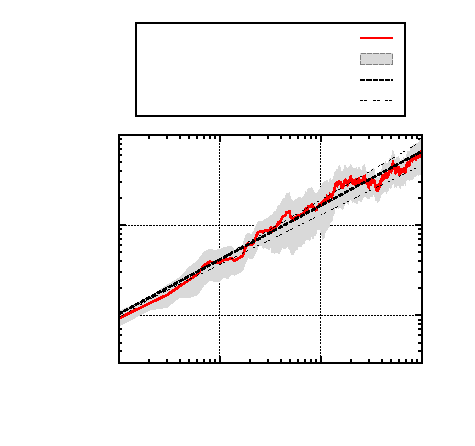
\includegraphics{MSD_error_s}}%
    \gplfronttext
  \end{picture}%
\endgroup

}}
\caption{Dubbellogplott av de olika sorternas MSD för celler i dvala med felgränser och möjliga anpassningar. De olika MSD:erna beräknades med \eqref{eq:MSD_S} respektive \eqref{eq:MSD_s}. Felgränserna är satta som konfidensintervall med 95\,\% konfidens. Med felgränserna syns att exponenten kan variera omkring $\pm 0,05$; detta visar sig också vara fallet för celler i log-fas.}
\label{fig:MSD_error}
\end{figure}
%\restoregeometry

Jämförs exponenterna i potensanpassningen mellan cellerna i dvala och log-fas, (a) respektive (b) i \figref{fig:MSD}, finns en viss skillnad. Exponenten för cellerna i dvala är $0,6$ mot log-fas-cellernas $0,8$. Med osäkerhetsgränser som i \figref{fig:MSD_error} syns att dessa värden på exponenterna själva får en osäkerhet på ungeför $\pm 0,05$. Även om \figref{fig:MSD_error} bara visar detta för partiklar från celler i dvala så gäller samma osäkerhet i exponenten för celler i log-fas.

Även med felgränserna i \figref{fig:MSD_error} för exponenterna syns dock att båda processerna ändå är exempel på subdiffusion. Alltså att partiklarnas MSD beror av tiden som ett potenssamband med exponent mindre än $1$. Subdiffusion är en avvikelse från klassiska brownsk rörelse, där exponenten enligt \eqref{eq:MSD_brown} ska vara $1$. 


I \figref{fig:MSD} syns att MSD:n från \eqref{eq:MSD_s} är som förväntat mer ojämn än den stationära då färre medelvärden tas. Vidare ser $S$ och $s$ ut att ha ungefär samma värde i samtliga fall. Detta beror på normeringen från avsnitt~\ref{sec:resultat-storleksberoende} som använts för att normera mot inensiteten. Men då det bara är lutnigen, i dubbellogplot, på MSD:n som är intressant så påverkas inte resultaten av vilka absoluta värden MSD:n har.






\section{Anisotropi i partikelrörelsen}
Om man misstänker att cellens inre struktur påverkar partikelrörelserna skulle eventuell anisotropi kunna ge ett bidrag till dessa. Alltså ifall det finns föredragna riktningar för partikeln att röra sig i. Ett sätt att undersöka detta är genom att betrakta koordinaternas kovariansmatris som är en matris med de olika koordinaternas statistiska andramoment:
\begin{equation}
C_{ij} = \frac{1}{N} \sum_{n=1}^{N} 
\left(r_i^{(n)}r_j^{(n)} -\bar{r}_i\bar{r}_j \right),
\end{equation}
där $r_i^{(n)}$ är den $i$:te koordinaten ($x$ eller $y$) i den $n$:te datapunkten och $\bar{r}_i$ är den $i$:te koordinatens medelvärde. På matrisform kan $C$ skrivas som
\begin{equation}\label{eq:C_matris}
C=
\begin{bmatrix} 
\ev{x^2}-\ev{x}^2 & \ev{xy}-\ev{x}\ev{y}\\
\ev{yx}-\ev{x}\ev{y} & \ev{y^2}-\ev{y}^2
\end{bmatrix}.
\end{equation}

Notera hur snarlik $C$ är med tröghetsmatrisen för en kropps olika tröghetsmoment som uppkommer i mekaniken. Och precis som i mekaniken kan man hitta två principalaxlar genom att ta fram dess egenvektorer och diagonalisera matrisen. I mekaniken svarar principalaxlarna mot de riktningar av rörelsemängdsmoment som är oberoende av rotation längs andra axlar. I de här statistiska sammanhangen finns det en liknande tolkning nämligen att principalaxlarna svarar mot de riktningar i cellen där rörelserna är oberoende av varandra. Egenvärdena i dessa två riktningarna svarar mot variansen i den oberoende koordinaten längs med den riktningen.

För att ur kovariansmatrisen få ut ett mått på hur isotropt partikeln rör sig kan man undersöka asymmetrimåttet~\cite{Rudnick_Asphericity1986}
\begin{equation}\label{eq:asph.}
    A_d=\frac{\sum_{j=1}^d\sum_{i<j} 
\ev{(\lambda_i-\lambda_j)^2} }{
(d-1) \ev{(\sum_{j=1}^d \lambda_j)^2}}
\end{equation}
i $d$ dimensioner, kallat \emph{asfärisitet}. Egenvärdena själva svarar som sagt mot variansen i de olika riktningarna, vilket motsvarar hur mycket partikeln har rört sig i respektive rikting. Hade positionerna varit helt isotropt fördelade så hade alltså $A=0$, om partikeln bara hade rört sig längs en linje blir istället $A=1$.
I två dimensioner förenklas \eqref{eq:asph.} till 
\begin{equation}\label{eq:asph._2D}
    A=\frac{\ev{(\lambda_1 - \lambda_2)^2}}{\ev{(\lambda_1 + \lambda_2)^2}}.
\end{equation}

\subsubsection{Tillämpning av asfärisiteten}
Man kan enkelt visa att egenvärdena till kovariansmatrisen i \eqref{eq:C_matris} uppfyller~\cite{Hong_asymmetri1998}
\begin{equation}
\begin{aligned}
\lambda_1+\lambda_2 
&= \ev{x^2}-\ev{x}^2+\ev{y^2}-\ev{y}^2 
\\
\abs{\lambda_1-\lambda_2} 
&=\sqrt{\left(
            \left(\ev{x^2}-\ev{x}^2\right)^2
            -\left(\ev{y^2}-\ev{y}\right)^2
        \right)^2 
        +4(\ev{xy}-\ev{x}\ev{y})^2
}.
\end{aligned}
\end{equation}
För en given fördelningsfunktion med ändliga moment blir det därmed nu möjligt att beräkna denna kvot teoretiskt.

För en obegränsad Wienerprocess i $d$ dimensioner fås~\cite{Rudnick_Asphericity1986}
\begin{equation} \label{eq:Asphericity_Brownian}
    A_d^\text{(Wierner)}=\frac{2(d+2)}{5d+4}.
\end{equation}
För två dimensioner blir $A_2^\text{(Wierner)}=\nicefrac{4}{7}$. Detta innebär att även långvariga slumpvandringar i snitt kommer att uppvisa viss anisotropi.

För fBm fås en formel i två dimensioner som gäller i gränsen där antalet mätpunkter blir mycket stort ~\cite{Hong_asymmetri1998}
\begin{equation} \label{eq:A_fBm}
A=2-
\frac{\frac{1}{2(H+1)^2}}{\frac{1}{2(H+1)^2}+\frac{2H+1}{4(4H+1)}-\frac{1}{4H+3}-\frac{\Gamma^2(2H+2)}{\Gamma(4H+4)}},
\end{equation}
där $H$ är Hurst parametern som karakteriserar rörelsen och $\Gamma$ är gammafunktionen. För $H=\nicefrac{1}{2}$ fås en vanlig brownsk rörelse med motsvarande  asymmetrimått $A=\nicefrac{4}{7}$ vilket stämmer överens med ekvation \eqref{eq:Asphericity_Brownian} för $d=2$. Samma värde fås även approximativt för CTRW-modellen \cite{Ernst_ACTRW2012} då denna rörelse vid varje tidsögonblick ser ut som brownsk rörelse. \todo[color=lime]{Kanske kan förklaras bättre?}

%Även http://iopscience.iop.org/article/10.1088/0305-4470/19/4/004/pdf



 
\subsection{Simulering och numerisk beräkning av asymmetrimått} 
\label{sec:sim_asym}
Istället för att bara direkt beräkna $A$ enligt \eqref{eq:asph._2D} för den undersökta datan och några olika modeller kan man också studera fördelningen av måttet 
\begin{equation}\label{eq:asym}
\mathcal{A} =
\frac{(\lambda_1 - \lambda_2)^2}{(\lambda_1 + \lambda_2)^2}.
\end{equation}
Här ska det dock påpekas att det inte går att få $A$ från  $\ev{\mathcal{A}}$ eftersom \eqref{eq:asph._2D} består av ett väntevärde i både täljare och nämnare. Eftersom $\mathcal{A}$ alltså skiljer sig så från $A$ går det heller inte lika enkelt att göra teoretiska beräkningar, vilket gör att fördelningen av $\mathcal{A}$ får undersökas med Monte Carlo-simuleringar.


%Eftersom en mätning bara kan bestå av ett ändligt antal datapunkter kan även en äkta, isotrop brownsk rörelse ge upphov till $\mathcal{A}>1$. Vidare är \emph{kvoten} mellan egenvärden inte linjär, vilket gör en teoretisk analys av fördelningarna mycket svår. För att ändå kunna säga något om den riktiga datan kan man ganska enkelt ta fram en fördelning för $\mathcal{A}$ för några olika modeller genom simulering. 

De modeller som testats är en vanlig Wienerprocess, en Wienerprocess med ett ''mätbrus'' pålagt och en Ornstein-Uhlenbeck-process. Tyvärr simulerades inte \todo{Om inte någon annan vill ta/har tagit sig an detta.}fBm och CTRW då dessa modeller är betydligt mer komplexa och behöver mer avancerade simuleringsalgoritmer. 
Från dessa processer samt från datan över partikelrörelsen erhölls olika värden på $A$ och fördelningar av $\mathcal{A}$. 


I Wienerprocessen simulerades partikelns position i varje ny tidpunkt genom att gå ett normalfördelat steg från positionen i den förra tidpunkten. Detta kan skrivas som
\begin{equation}\label{eq:sim_wiener}
x_{i+1} = x_i + \sigma_\text{steg}\delta 
\qcomma  \delta \sim N(0, 1)
\end{equation}
och där $x_1=0$. Sedan gör man samma sak för $y$. Eftersom $\mathcal{A}$ ger ett mått på hur mycket partikeln \emph{föredrar en viss riktning}, finner man att värdet på $\sigma_\text{steg}$ inte påverkar fördelningen -- så länge $\sigma_\text{steg}$ är samma för både $x$ och $y$. Detta blir uppenbart när man tänker på att \eqref{eq:sim_wiener} kan skrivas som 
\begin{equation}
x_{i+1} =\sigma_\text{steg}\,x'_{i+1} = \sigma_\text{steg}\left( x'_i + \delta \right) 
\end{equation}
Alltså att $\sigma_\text{steg}$ bara är en multiplikativ konstant framför positionen.

För att istället simulera en Wienerprocess med mätbrus användes \eqref{eq:sim_wiener} för att först simulera själva Wienerprocessen för att sedan \emph{efteråt} addera en slumpad brusterm $\sigma_\text{brus}\eta$ till varje position $x_i$. Positionerna i simuleringen med brus ges alltså av
\begin{equation}
\hat{x}_{i} = x_i + \sigma_\text{brus}\eta 
\qcomma  \eta \sim N(0, 1).
\end{equation}
Den väsentliga skillnaden mot en ren Wienerprocess är att mätbruset $\eta$ inte påverkar nästkommande position. Till skillnad från den rena Wienerprocessen så kommer värdena på $\sigma_\text{steg}$ och $\sigma_\text{brus}$ att påverka $\mathcal{A}$, men enligt samma argument som ovan kommer bara kvoten $\nicefrac{\sigma_\text{brus}}{\sigma_\text{steg}}$ vara det som påverkar. Detta gör att simuleringarna med mätbrus går att genomföra med olika värden på parametern $\nicefrac{\sigma_\text{brus}}{\sigma_\text{steg}}$ för att få olika fördelningar av~$\mathcal{A}$. 

Ornstein-Uhlenbeck-processen i \eqref{eq:SDE_o-u} simulerades genom att använda derivatan för tidsutveckling och genom att sätta $\bar{x}=0$. Man får då
\begin{equation}
x_{i+1} = x_i + \Delta{t}\,\pd_{t}x  = (1-k) x_i +  \sigma_\text{steg}\delta 
\qcomma  \delta \sim N(0, 1),
\end{equation}
där $x_1=0$. Notera här att den styrande parametern i simuleringarna är $k=\gamma\Delta{t}$, samt att $\sigma_\text{steg}$ på samma sätt som för den rena Wienerprocessen kan väljas godtyckligt utan att påverka $\mathcal{A}$. 

Samtliga simuleringar har gjorts med 1000 steg och 100\,000 upprepningar. Antalet steg valdes för att simuleringarna ska efterlikna den studerade datan -- som består av 1000 sparade positioner för varje partikel. Däremot kan upprepningarna väljas godtyckligt. Då valdes 100\,000 för ge tillräckligt jämna fördelningar.\todo{Borde man flytta det här till resultatet?}

%Vill Emelie lägga in något resultat om detta så får hon gärna lägga tillbaks det här stycket
%Eftersom resultatet för asymmetrimåttet i ekvation \eqref{eq:A_fBm} gäller för riktigt långa mätningar medan den data som analyseras i detta arbete är ganska begränsad kan man försöka simulera fram sannolikheter istället. Genom att simulera många mätserier för samma antal steg och antal partiklar som i datan kan man bedöma sannolikheten att det framräknade asymmetrimåttet till exempel skulle ha kommit från en ren klassisk brownsk rörelse. 


\subsection{Resultat -- partikelrörelserna är isotropa och behöver inte delas upp i anpassade koordinater}
\label{sec:resultat-isotropi}

\begin{figure}\centering
\input{bilder/partiklar/isotropi_asymmetri.tex}
\caption{Fördelning av asymmetrimåttet $\mathcal{A}$ enligt \eqref{eq:asym}, visat som sannolikheten att $\mathcal{A}$ är \emph{större} än ett visst värde $a$.
Graferna visar att de partiklar från celler i log-fas, i det här avseendet, beter sig som en Wiernerprocess. Partiklarna från celler i dvala beter sig däremot mer isotropt än en vanlig Wienerprocess; deras betende skulle kunna modelleras som en Wienerprocess med pålagt brus med $\nicefrac{\sigma_\text{brus}}{\sigma_\text{steg}} = 6$ eller som en Ornstein-Uhlenbeck-process med tidskonstant $\nicefrac{1}{\gamma} =\unit[4]{s}$.
}
\label{fig:asymmetri}
\end{figure}

\begin{table}
\centering
\caption{Värden på asfärisitetsen $A$ enligt \eqref{eq:asph._2D} för de undersökta partiklarna och processerna. De simulerade värden kommer från simuleringarna gjorde med 1000 steg och 100\,000 upprepningar med samma parametrar som i \figref{fig:asymmetri}. De små osäkerheterna i de simulerade värdena beror på att medelvärdena kommer från så många simuleringar. Osäkerheterna i de angivna värdena är angivna med en standardavvikelse. 
%Läsaren påminns om att en helt cirkulärt symmetrisk fördelning svarar mot $\mathcal{A}=0$, medan $\mathcal{A}=1$ svarar mot att positionerna ligger på en linje.
}
\label{tab:asph._values}
\begin{adjustbox}{center}
\begin{tabular}{l|c|c|c|c|c|c|}\cline{2-7}
%första raden
& \multicolumn{2}{c|}{Uppmätta} 
& Teoretisk 
& \multicolumn{3}{c|}{Simulerade}
\\ \cline{2-7}
%Första delen av andra raden
& \multirow{3}{*}{Log-fas} & \multirow{3}{*}{Dvala }%mätdata
& \multicolumn{3}{c|}{Wienerprocesser }%Wiener 
& 
\\ \cline{4-7}%\cline{2-3}\cline{6-7}
& & & \multicolumn{2}{c|}{\multirow{2}{*}{utan mätbrus} }%Wiener
& med mätbrus  & O-U-process %simulerade brus och O-U
\\
%Andra delen av andra raden
& & &\multicolumn{2}{c|}{}
& $\nicefrac{\sigma_\text{brus}}{\sigma_\text{steg}} = 6$ & $\nicefrac{1}{\gamma} =\unit[4]{s}$
\\\hline
%Sista raden, med värden
\multicolumn{1}{|l|}{$A$:}
& $0,41\pm 0,23$ & $0,49\pm 0,15$ %mätdata
& $\nicefrac{4}{7}\approx 0,571$ & $0,570\pm 0,005$ %Wiener
& $0,43\pm 0,003$ & $0,34\pm 0,002$ %brus och O-U
\\ \hline
\end{tabular}
\end{adjustbox}
\end{table}

\todo[color=lime]{Ska vi säga något om att banorna verkade vara like assymetriska?}
Som kan ses i \figref{fig:asymmetri} skiljer sig den simulerade asfärisiteten $\mathcal{A}$ mellan partiklar från celler i dvala och de i log-fas. Båda fallen har fördelningar som svarar mot en rörelse som är minst lika isotrop som Wiernerprocessen -- under de undersökta tidsskalorna. Vidare ses att partiklarna från celler i dvala får en fördelning av $\mathcal{A}$ med betydligt lägre sannolikhet för högre $\mathcal{A}$-värden, svarande mot mer asymmetriska rörelser. Skillnaden mellan cellfaserna tyder på att något förändras i cytoplasman när cellen går i dvala, något som påverkar partikelrörelserna. 

Om istället det riktiga asfärisitetsmåttet, $A$ från \eqref{eq:asph._2D}, betraktas erhålls värdena i \tabref{tab:asph._values} där uppmätta, teoretiska och simulerade värden presenteras med felgränser. Det bör dock nämnas att det teoretiska värdet gäller i gräns mot när antalet steg går mot oändligheten medan de simulerade och uppmätta värdena beräknats från diskreta datamängder. Viss avvikelse kan därför vara att vänta. Från tabellen ses att de uppmätta värdena på $A$ för partiklarna, $0,41\pm0,23$ för log-fas och $0,49\pm0,15$ för cellerna i dvala, på grund av sin stora felgräns omsluter både resultatet för Wienerprocessen och O-U-processen med tidskonstant $\nicefrac{1}{\gamma}=\unit[4]{s}$. Partikelrörelsen är alltså minst lika isotrop som dessa båda processer.

\section{PSD}



%Lite om hur det borde se ut om det var brownsk
Som sagts i avsnitt~\ref{sec:white_noise} så beskriver Wiernerprocessen brownsk rörelse matematiskt. Detta gör att Man kan få PSD:n för brownsk rörelse genom att undersöka Wiernerprocessen. En sak som också nämndes i avsnitt~\ref{sec:white_noise} är att Wienerprocessen kan tolkas som \emph{integralen av vitt brus}. Så PSD:n för Wienerprocessen kan alltså uttryckas med hjälp av den konstanta PSD:n för vitt brus.
På ett lite handviftande vis bör alltså 
\begin{equation}
S_\text{Wiener} (f) \propto f^{-2} S_\text{Vitt brus}(f) \propto f^{-2}.
\end{equation}
Här har man utnyttjat PSD:ns koppling till Fouriertransformen, så att integrering kan skrivas som att transformen multipliceras med $(\ii f)^{-1}$. Sedan följer kvadraten av att PSD använder beloppskvadraten av transformen. 

\subsection{Resultat -- }


\section{Diskussion}
\todo[inline]{Inga tomma rubriker}


\subsection{MSD -- subdiffusivt beteende pekar mot att vanlig brownsk rörelse inte räcker som förklaringsmodell}
%Klippt från resultatdelen
Då MSD:n ger en vink om hur snabbt partiklarna sprids verkar partiklarna i cellerna i dvala diffundera långsammare än partiklarna i de aktiva cellerna. De undersökta cellernas metabola tillstånd verkar alltså påverka diffusionen i cytoplasman vilket bekräftar resultat från tidigare studier~\cite{Parry_etal2014}. Dessa studier har, liksom här, utförts på celler utan motorprotein. Detta utesluter förklaringsmodellen där de utpekas som största bidragsfaktor som möjlig förklaring det det observerade fenomenet. 




%\subsection{Intensitetskorrigering}

\subsection{Brusnivån är lägre än väntat}
Som resultaten i avsnitt~\ref{sec:resultat-storleksberoende} visar är brusnivån ganska låg, omkring \unit[5]{nm}. Detta är är lågt, vilket skulle kunna tyda på att metoden är bristfällig.

För det första kan det kännas märkligt att ens kunna prata om observationer av nanometerstora röreler gjorda med ett \emph{optiskt} mikroskop. Instinktivt borde det inte gå att upplösa något som är mindre än ljusvåglängden, på flera hundra nanometer. Och om inte ljusets våglängd skulle vara begränsande, så borde i alla fall bildsensorns pixelstorlek sätta en nedre gräns i upplösningen. Men så är faktiskt inte fallet. Det går att få subpixelnoggannhet~\cite{Saunter2010} genom att utnyttja olika databehandlignstekniker som hittar centrum på en flera pixlar bred ljusfäck på kamerasensorn.

Med detta sagt behöver man dock komma ihåg att sådan subpixelnoggrannhet typiskt ger en maximal upplösning på omkring en tiondels pixel~\cite{Saunter2010}. I det här fallet skulle detta svara mot cirka 11\,nm upplösning. Detta är också den brusnivå som \cite{Midtveldt_etal2016} kom fram till när de analyserade samma data. De använde sig dock av en metod där de undersökte partiklarnas PSD för att hitta en brusbakgrund. 


Från \figref{fig:storleksberoende}, framför allt (c) och (d), kan man dock se att $\sigma_\text{brus}=\unit[11]{nm}$ verkar vara en överskattning. För om den faktiska brusnivån var \unit[11]{nm} så borde väldigt få mätpunkter hamna under den utmarkerade linjen för \unit[11]{nm}-brus i \figref{fig:storleksberoende}. Detta verkar endast vara fallet för log-fas i \figref{fig:storleksberoende}~(b), men tittar man på steglängderna i log-fas (d) så går de ner under \unit[11]{nm}-nivån.

Avslutningsvis bör dock också sägas att brusnivån på cirka \unit[5]{nm} kan vara lite i lägsta laget. Detta för att ju högre intensitet en partikel har, desto lättare blir det att lokalisera den i ett mikroskop. Och eftersom brusnivån i den här studien beräknades från de partiklar med högs intensitet, så kan det hända att den uppmätta mätosäkerheten blir lägre här för att den är lägre för de större partiklarna. Dock verkar ändå \unit[5]{nm} vara den bättre uppskattningen.





\subsection{Isotropi}

En anledning att studera isotropin är att bedöma hurvida det finns en föredragen rikting i cellerna. Hade så varit fallet hade $A$ varit större för partiklarna än för Wienerprocessen. Detta skulle i så fall antyda om att det skulle finnas strukturer i cellen som påverkar partikelrörelsen. Det skulle då vara befogat att studera rörelserna längs dessa föredragna riktingar separat genom att till exempel införa normal- och tangentialkoordinater. Från avsnitt~\ref{sec:resultat-isotropi} visar sig dock detta \emph{ej} vara fallet.

Genom att gå över till normal och tangentialkoordinater när detta inte är motiverat riskerar att leda till metodfel i dataanalysen. Ett sådant koordinatbyte kan leda till att man hittar mönster som egentligen inte finns men som normaltsett uppstår, även i vanlig brownsk rörelse. En stark motivering bör därför föregå ett sådant koordinatbyte. Eftersom det inte finns några indikationer på att det skulle finnas en strukturell anisotropi har inga sådana koordinatbyten gjorts i den här studien.


En annan anmärkningsvärd sak är att de olika asymmetrimåtten skiljer sig så tydligt åt mellan cellfaserna. Fördelningen av $\mathcal{A}$ från \figref{fig:asymmetri} tyder på att partiklar från celler i dvala beter sig mer isotropt, medan värden på $A$ i \tabref{tab:asph._values} pekar på ett överlapp mellan partiklar från celler i dvala eller log-fas. Det är till och med så att värden i \tabref{tab:asph._values} eventuellt antyder om att partiklar från celler i log-fas beter sig mer isotropt, men det är för stora felmarginaler för att kunna dra några slutsatser.

\subsubsection{Mätbrus är ingen tillfredsställande förklaring}
Förhållandet mellan standardavvikelsen för bruset och steglängden $\nicefrac{\sigma_\text{brus}}{\sigma_\text{steg}}$ varierade i den undersökta datan på grund av olika rörlighet för olika partiklar. Större partiklar tenderade att förflytta sig kortare sträckor än de små partiklarna. Från beräkningarna av medelstegen i \figref{fig:storleksberoende}~(c) och (d) visade det sig också att medelstegens standardavvikelse var omkring $\unit[10\pm 5]{nm}$. Vilket, med $\sigma_\text{brus}=\unit[5]{nm}$ från avsnitt~\ref{sec:resultat-storleksberoende}, skulle svara mot $\nicefrac{\sigma_\text{brus}}{\sigma_\text{steg}}=0.5\pm 0.2$. Det verkar alltså högt osannolikt att isotropin för partiklar i celler i dvala skulle kunnat ha uppstått från så brusig data som användes i avsnitt~\ref{sec:resultat-isotropi}. 

En annan anledning att brusig data inte kan förklara avvikelsen för celler i dvala i \figref{fig:asymmetri}, är att pertiklarna från celler i log-fasen inte påverkades trots att brusnivån borde vara samma i båda fallen. Man skulle kunna argumentera för att $\nicefrac{\sigma_\text{brus}}{\sigma_\text{steg}}$ ändå kan skilja sig mellan de olika cellfaserna för att $\sigma_\text{steg}$ skulle kunna variera. \figref{fig:storleksberoende}~(c) och (d) visar dock tydligt hur steglängderna mer eller mindre är de samma mellan cellfaserna.

Hypotesen, att mätbrus skulle kunna förklara avvikelserna från brownsk rörelse, kan alltså förkastas även då värdena för asfäriteten i \tabref{tab:asph._values} och dess fördelnigen \figref{fig:asymmetri} ser ut att kunna stämma. 

Den andra förklaringsmodellen, Ornstein-Uhlenbeck-processen, diskuteras vidare i dess egna avsnitt längre ner. För tillfället räcker det att säga att den är mer tillfredsställande än brusmodellen. 



\subsubsection{Inget intensitetsberoend i asymmetrin pekar mot storlekoberoende partikelbindning}
I isotropimätningarna användes ingen intensitetskorrigering. Den huvudsakliga anledningen till detta var att oavsett hur stora partiklarna är så borde de ändå ha samma rörlighet i olika riktningar. Man skulle dock kunna invända mot detta genom att mena att en större partikel skulle vara hårdare bunden. Detta skulle motsvara en mindre tidskonstant i en Ornstein-Uhlenbeck-modell, vilket skulle ha gett mer isotropa fördelningar för större partiklar.

När man undersöker om det finns något beroende mellan $\mathcal{A}$ och partikelintensiteten, så finner man dock ingen tydlig trend. Detta gäller oavsett vilken cellfas som undersöks.
Intensitetsoberoendet här verkar alltså peka mot att olika stora partiklar ändå har samma bindningsstyrka i en Ornstein-Uhlenbeck-modell. 



%Om sambandet mellan intensitet och partikelstorleken påverkar resultatet

%Byter man till normal- och tangential-koordinater bygger man in ett bias som påverkar resultaten till att det verkar finnas egenskaper som egentligen inte finns. 
%Av slumpskäl kommer vissa vägar att vara mer raka än andra medan andra får mer symmetriska banor.



\subsection{Ornstein-Uhlenbeck-modellen kan inte förklara subdiffusion men skulle kunna användas i andra sammanhang}

Notera att för $\gamma\Delta{t}\ll 1$ så ger \eqref{eq:MSD_o-u} att 
$\ev{(x(t)-x(t') )^2}\widetilde{\propto}\,\Delta{t}$. Detta betyder alltså att Ornstein-Uhlenbeck-processen inte kan användas för att förklara tidigare observerade avvikelser\cite{Hofling&Franosch2013} i partiklars MSD. Dock så är den här modellen bara en första utveckling av brownsk rörelse, så det är inte så förvånane att den inte skulle klara av att förklara allt. Men förhoppningsvis skulle den kunna förklara vissa beteenden som observeras. 


\subsubsection{Modell för att förklara skillnad i isotropi mellan cellfaserna}



\subsection{Uppskattning av Hurstparametern och fBm som modell för partikelrörelse i celler}

Då Hurstparametern för en fBm återfinns i många förutsägelser för rörelsen kan denna uppskattas från flera håll, bland annat från exponenten i MSD:n \eqref{eq:fBm_MSD} och som parameter i asfärisiteten \eqref{eq:A_fBm}. 
I figur \figref{fig:MSD} presenterades värdena för MSD:n för datan till att vara $0,65\pm0,01$ för cellerna i dvala och $0,80\pm0,05$ för log-fas cellerna. Detta svarar via \eqref{eq:fBm_MSD} mot $2H$ vilket ger $H=0,325\pm0,005$ och $H=0,40\pm0,03$ för cellerna i dvala respektive log-fas cellerna.
Beräknade värden för asfärisiteten presenteras i tabell \tabref{tab:asph._values}. För cellerna i dvala fås $H=0,41\pm 0,23$ och för log-fas cellerna $H=0,49\pm 0,15$. Motsvarande H-värde fås approximativt från \eqref{eq:A_fBm} till att bli $H=0,36\pm0,20$ respektive $H=0,43\pm0,13$, om relativa felet bevaras. Snitten mellan de två uppskattningarnas intervall är nollskilda för respektive cellfas vilket ger viss rimlighet till fBm som modell för partikelrörelse i celler. Den stora felgränsen i uppskattningen av H från asfärisiteten gör dock detta påstående svagt.

Båda dessa uppskattningar av $H$ ger ett värde som med stor sannolikhet befinner sig under $\nicefrac{1}{2}$, svarande mot en rörelse med positiv korrelation mellan två positioner i rörelsen, dvs att partikeln tenderar att röra sig bort från startpositionen. Detta kan vara ett rimligt resultat under de tider som studeras här då cellens begränsade utbredning inte begränsar rörelsen. För längre samplingstider skulle man dock kunna förvänta sig $H>\nicefrac{1}{2}$, där negativ korrelation fås i rörelsen och partikeln tenderar att röra sig tillbaka mot startpositionen. 

Som modell skulle fBm med ovanstående beräkningar nog kunna beskriva vissa egenskaper hos partikelrörelse i celler, åtminstone approximativt. Modellen ger dock inte någon fysikalisk beskrivning till rörelsens egenskaper utan bara matematiska förutsägelser. Denna avsaknad av koppling mellan den mikroskopiska, underbyggande fysiken och de makroskopiska, observerade egenskaperna gör fBm mindre tilltalande som kandidat för den alltäckande modellen för partikelrörelse i celler. Vidare studier på partikelrörelse i jästceller skulle kunna bekräfta fBm:s användbarhet som matematisk modell, men som fysikalisk modell brister den i sin avsaknad av tydlig fysikalisk tolkning.
\todo[color=lime]{Ska vi vara så här ärliga?}

\subsection{Något om CTRW}
Stationär process $->$ CTRW inte så aktuell.

\todo[color=lime,inline]{Ska vi säga något om CTRW som modell här?}

%Bara en liten kodsnutt som behövs när man kompilerar lokalt
%%% Local Variables: 
%%% mode: latex
%%% TeX-master: "00main.tex"
%%% End: 

\chapter{Strängars rörelse i vätskor}

%\subsubsection{Strängrörelser inom cellen}
Aktinfilament är polymerer som utgör en viktig byggsten för cellens cytoskelett och transportväg för motorprotein vilka formar och bidrar till cellens utseende, dynamik och stadga. För att kunna ge en mer detaljerad beskrivning av dessa egenskaper är studien av enstaka aktinfilaments dynamik av stort intresse. I detta arbete har olika dynamiska egenskaper för aktinfilament studerats, både för filament som fluktuerar fritt i en vätska och filament instängda i en rektangulär kvasi-2D-mikrokanal -- alltså att kanalen har försumbart djup. Mikrokanalen är till för att simulera beteendet hos aktinfilament i cytoskelettet där det omges av andra filament och därmed har en begränsad möjlighet till rörelse.

Det här kapitlet börjar med en översikt över hur mikroskopidatan behandlas för att kunna användas i studien av strängarna. Därefter presenteras och undersöks en modell för fria strängröreler samt en modifikation av modellen som beskriver inneslutna strängar. Till sist beskrivs en undersökning av strängarnas egenmoder.

\section{Undersökt data}
Datan som analyseras för strängrörelse i vätska är sammma som Köster et~al.~\cite{Koster_etal2005,Koster_etal2007} använde och består av filmer av aktinfilament som tillåts röra sig i en vätska. Dessa strängar hade en längd kring 10--30\,\micro{m} och befann sig i kanaler av olika bredd. %\todo{Kanaler av olika bredd?Inte helt konsistent med stycket nedan}

Två typer av strängar studeras: fria strängar i breda kanaler och inneslutna strängar i en kvasi-2D-mikrokanal. Upplösning på filmerna är 10 bilder per sekund. Rörelsen utfördes till största del i två dimensioner då kanalernas djup var litet i förhållande till kanalernas och filamentens bredd.


\subsection{Polynomanpassning för strängarna} \label{sec:polynomanpassning}

\begin{figure}\centering
\input{bilder/strangar/strang_anpassning.tex}
\caption{
Utdrag med pixelpositioner från en av strängarna tillsammans med polynomanpassningen som användes i denna studie samt en spline mellan pixlarna. Utdraget är bara av en mycket liten del av strängen för att enskilda pixlar ska synas.
Eftersom exempelvis tangent- och normalvektorer till strängarna är intressanta att studera behövs mjuka anpassningar till rådatan så att det går att derivera längs med strängen. 
}
\label{fig:strang_anpassning}
\end{figure}

Mätdatan för strängarna bestod vid varje tidpunkt av en matris med element motsvarande pixlarna på kameran. Datan var förbehandlad och strängen representerades som ett antal 1:or i en annars tom matris. 
För att kunna arbeta effektivt med strängarna behövs dock någon form av anpassning till dessa ''pixlar''. Bland annat behövs mjuka anpassningar för att kunna ta fram tangent- och normalvektorer i en godtycklig punkt längs med strängen. I \figref{fig:strang_anpassning} visas ett litet utdrag av en sträng med pixlepositioner och anpassningar. 

För att kunna göra en anpassning behövs först och främst en parameter som kan användas för att anpassa mot. 
Strängens position i varje tidsögonblick parametriserades med en normerad båglängdsparametern $s\in[0,1]$. Alltså att $s$ svarar mot hur stor andel av strängens längd som ligger bakom punkten svarande mot det $s$-värdet. 
För att i MATLAB bilda båglängsdparametern sorterades först punkterna i en ordnad följd längs med strängen. Efter detta uppskattades hur långt längs med strängen varje pixel på strängen låg. Detta gjordes genom att ackumulera längderna på de förbindande linjerna mellan varje pixel. På så sätt erhålls ett $s$-värde för varje pixel och nu kan en anpassnings göras av pixlarnas $x$- och $y$-koordinaterna mot $s$.

I den här studien valde vi att anpassa positionerna i varje tidpunkt med ett polynom av grad $20$ för vardera $x_t$ och $y_t$ enligt
\begin{equation}\label{eq:anpassning}
x_t(s) = \sum_{n=0}^{20} a_n^{(t)} \,s^n,
\end{equation}
där koefficienterna $a_n^{(t)}$ anpassades med hjälp av MATLABs \texttt{polyfit}-funktion till varje pixels position och $s$-värde. På samma sätt kunde även ett polynom för $y$ anpassas. Att det skulle krävas ett 20-gradspolynom för att följa strängen syns inte i \figref{fig:strang_anpassning} på grund av att figuren bara visar en mycket liten del av strängen. Graden behövde dock vara så hög för att de anpassade polynomen skulle kunna följa strängen bra längs med hela strängens längd. 

Sedan får inte graden väljas mycket högre än cirka 20 för att inte få med andra artefakter från polynomanpassning såsom en variant av Runges fenomen\cite{Gustafsson_LaNa}. Alltså att polynomet börja svänga kraftigt för att exakt gå igenom alla punkter som det ska anpassas till. Detta är i regel ett problem för interpolationer och inte anpassningar, men om gradtalet väljs ungefär lika stort som antalet punkter som ska anpassas så tenderar anpassningen att bli som en interpolation.


\subsubsection{Alternativa metoder för att anpassa en kurva till strängdata}

\figref{fig:strang_anpassning} visar också en kubisk splineinterpolation som också är ett sätt som använts för att anpassa en kurva till strängen~\cite{Koster_etal2005,Koster_etal2007}. Dock anser vi att beteendet som splineinterpolationen uppvisar i \figref{fig:strang_anpassning} inte speglar den verkliga strängens form. Det är inte särskilt troligt att den verkliga strängen helt skulle följa varje pixel, utan det är mer rimligt att den verkliga strängen följer en sorts medelposition av pixlarna. 

En sak som ytterligare talar för att splineinterpolation inte är en optimal anpassningsmetod är svängningarna\footnotemark{} som syns i \figref{fig:strang_anpassning} mellan pixlarna. Dessa svängningar är över längdskalor som är mindre än mikroskopets upplösning. Det är alltså inte motiverat att använda sig av en metod som ger information som inte går att observera. 
\footnotetext{Dessa svängningar är dock inte ett exempel på Runges fenomen. Eftersom en kubisk spline är flera olika tredjegradspolynom fås inte beteendet från ett höggradit polynom\cite{Gustafsson_LaNa}. }


\subsection{Mäta avstånd från jämviktsläge}

\begin{figure}
\centering
\resizebox{0.8\textwidth}{!}{
    \input{bilder/strangar/transv_avst.pdf_t}
}
\caption{Schematisk skiss av hur transversella avståndet från medelsträngen mäts. I varje tidpunkt jämförs medelsträngens position, $\mathbf{r}_0(s)$, med den momentana strängens position, $\mathbf{r}(s, t)$, för samma $s$-värde -- $s$ är en parameter som motsvarar en viss sträcka längs med strängen. För att få ett avståndsmått som kan växla tecken undersöks projiceringen av skillnaden i ortsvektor på medelsträngens normalvektor. 
}
\label{fig:transv_avst}
\end{figure}

I denna rapport har strängens translationsrörelse till stor del försummats genom att i varje tidpunkt placerat strängens masscentrum i origo. Givet detta är det intressant att studera huruvida strängarna fluktuerar kring något jämviktsläge. En uppskattning av jämviktsläget $\mathbf{r}_0(s)$ tas fram genom att beräkna medelvärdeskurvan som representerar strängrörelsen. 

Från detta jämviktsläge har det transversella avståndet beräknats enligt 
\begin{equation}
A_s(t) = \mathbf{n}_0(s)\cdot\Big(\mathbf{r}(s,t)-\mathbf{r}_0(s)\Big),
\end{equation}
där $\mathbf{n}_0(s)$ är en normerad normalvektor till strängens jämviktsläge samt $\mathbf{r}(s,t)$ och $\mathbf{r}_0(s)$ är ortsvektorerna för momentansträngen respektive medelsträngen. Avståndet $A_t(s)$ motsvarar alltså projektionen av $(\mathbf{r}(s,t)-\mathbf{r}_0(s))$ på normalvektorn. Detta 
illustreras i \figref{fig:transv_avst}.








\section{Modeller för strängrörelser}

Aktinfilamenten precis som tidigare studerade partiklar påverkas av diffusionsprocessen inuti celler och således krävs stokastiska modeller för att beskriva rörelsen. En vanligt använd modell inom polymerfysiken är Worm Like Chain-modellen som beskrivs nedan. Vidare studeras en annan, fenomenologisk modell baserad på en langevinekvation. 



\subsection{Worm Like Chain-model}

Worm like chain modellen \cite{Milstein2013} (WLC) är en modell som ämnar beskriva fluktuationerna hos en semi-flexibel polymer. I modellen antas att polymeren är helt oelastisk, enbart påverkas av termiskt brus och styv på små längdskalor. Om polymeren fluktuerar fritt %utan att vara instängd i en mikrokanal 
ges en minimalistisk WLC beskrivning av att filamentets fluktuationer regleras av böjningsenergin. För en polymer med $N$ segment vardera med riktning \textbf{r}$_i$ och längd $\abs{r_{i}}=l$ samt polymerens böjstyvhet $\kappa$ ges böjningsenergin av
\begin{equation}
    H = -\kappa\sum_{i=1}^{N}\textbf{r}_{i}\cdot \textbf{r}_{i+1}.
\end{equation}
Maximalt bidrag till energin från två på varandra följande segment fås alltså om dessa har antiparallell riktning. Givet identiteten $\textbf{r}_{i}\cdot\textbf{r}_{i+1}=(2l^2-(\textbf{r}_{i+1}-\textbf{r}_{i})^2)/2$ kan summan skrivas om som en integral i gränsen då $N \to \infty$, $\kappa\to\infty$, $l \to 0$ men där produkten $\kappa l=\xi$ är finit som 
\begin{equation}\label{böj}
    H=\frac{\xi}{2}\int_{0}^{L}\!\dd{s}\,(\partial_{s}\textbf{t}(s))^2,
\end{equation}
där $\textbf{t}(s)$ är enhetstangentvektorn längs polymeren parametriserad med båglängden. Detta är den kontinuerliga WLC modellen \cite{Fixman_WLC1973} vilket ger en bra approximation av en polymer där längden av enskilda molekyler kan försummas. Korrelationen mellan två tangentvektorer medelvärdsbildat över tid ges av \cite{Landau1958}:
\begin{equation}
\ev{\textbf{t}(s)\textbf{t}(s+\Delta s)}=\ee^{-\frac{\abs{\Delta s}}{2L_{p}}},
\end{equation}
där $L_{p}=\frac{\xi}{k_{B}T}$ är kvoten mellan styvheten hos polymeren och termiska energin hos fluiden. Denna kallas \emph{persistence length} och ger ett mått på hur snabbt tangentkorrelationen avtar längs polymeren. I fallet då $\nicefrac{L_{p}}{L}>1$ sägs polymeren vara styv. 
För att öka noggrannheten kan även ett rumsligt medelvärde tas över tangentkorrelationerna, låt denna betecknas med ett heldraget streck. Tangentkorrelationen beror då inte längre av var på strängen korrelationen tas utan bara på avståndet mellan tangentvektorerna, $\Delta s$, och defineras som
\begin{equation}
\label{tangkorr}
    \ev{\cos\theta(\Delta s)}\equiv\overline{\ev{\mathbf{t}(s)\mathbf{t}(s+\Delta s)}}.
\end{equation}
Denna minimalistiska WLC modell förutspår alltså tangentkorrelationens utseende utifrån antagandet att strängen tillåts fluktuera fritt.



\subsubsection{Resultat -- mikrokanalen påverkar strängens tangentkorrelation}



För att undersöka hurvida mikrokanalen påverkar strängen beräknas tangentkorrelation enligt \eqref{tangkorr} för både ''fria'' samt inneslutna strängar. \todo[color=olive]{fixa figur på tangentkorrelation för sträng 1 samt 3.}I figur .. ses tangentkorrelationer för de olika proverna plottade med anpassade potensamband i $\Delta s$. Det ses att en sträng påverkas av en mindre mikrokanal då dess tangentkorrelation upplevs mer ihärdig. Persistence length fås för strängarna som \todo[color=olive]{kontrollera dessa}.. respektive .. . Eftersom strängarna i de olika proverna är snarlika aktinfilament, vars enda signifikanta skillnad är båglängd, tolkas skillnaden i persistence length som ett mått på hur en strängs möjlighet att fluktuera begränsas av mikrokanalen. 



\subsection{WLC-modell för sträng i mikrokanal}
\label{WLCkanal}


En mer sofistikerad modell kan konstrueras med avseende på mikrokanalens egenskaper och dess dynamik. Då interaktionen mellan strängen och kanalens väggar beskrivs som rent sterisk \cite{Koster_etal2007} kan denna approximeras med en parabolisk potential. Inför därför kraften $F \propto A(s)$ där $A(s)$ svarar mot strängens vinkelräta avstånd från centrum av kanalen. Potentiella energi med avseende på dessa avvikelser fås som
\begin{equation}
    H_{pot}=\int_{0}^{L} \!\dd{s} \, [\gamma A(s)^2],
\end{equation}
där $\gamma$ är en positiv konstant vilket avger styrkan hos potentialen. 

Då tangentvektorn till strängen kan defineras som $\mathbf{t}(s)=\partial_sA(s)$, adderas denna energi till den tidigare härledda hamiltonianen enligt

\begin{equation}
\label{Htot}
    H_{tot}=\int_{0}^{L}\!\dd{s}\,[\xi\partial_{s}^{2}A(s)^2 + \gamma A(s)^2],
\end{equation}
där första termen i integranden svarar mot energin enligt den tidigare modellen \eqref{böj}.

Hamiltonianen ger nu en modell av den kraft vilket kan tänkas verka på en sträng i en mikrokanal. Det ses att potentiella energin för strängen minimeras i fallet då denna är rak och fixerad längs kanalens centrum. Alltså återställer kraften eventuella avvikelser från jämviktsläget. Då avvikelserna uppstår på grund av termiska fluktuationer, vilka antas vara stokastiska, kan som tidigare i avsnitt~\ref{sec:brown} systemet betraktas med en langevinekvation. Då strängens intrinsiska tröghet, svarandes mot högre ordningens tidsderivata, försummas fås\cite{PhysRevE.60.4671}
\todo{jobba på övergången}

\begin{equation}
\label{mans}
    \partial_{t}A(t,s)=-\gamma A(t,s)+\xi \partial_{s}^{2}A(t,s)+\sigma \partial_{t}W(t,s).
\end{equation}
Fluktuationerna approximeras med termen $W(t,s)$, ett stokastiskt vitt brus vars intensitet är proportionellt mot reella talet $\sigma>0$. Notera hur langevinekvationen även beskriver tidsutveckling av systemet.

\todo{eget kapitel? ev. flytta ner beräkningarna i apendix}

Definera fouriertransformation som 
\begin{equation}
    \hat{A}(t,k)=\int_{-\infty}^{\infty}\!\dd{s}\, A(t,s)\ee^{-\ii sk}
\end{equation}
Genom fouriertransformation av \eqref{mans} fås en ordinär stokastisk differentialekvation av första ordningen
\begin{equation}
        \partial_{t}\hat{A}(t,k)=-\left(\gamma+\xi k^2\right)\hat{A}(t,k)+\sigma \partial_{t}\hat{W}(t,k).
\end{equation}
I fallet då $\gamma+\xi k^2=\zeta$ ses det att denna ekvation är ekvivalent med \eqref{eq:Brownian_SDE} vars lösning är känd. Vidare kan kovariansen formuleras likt \eqref{Brownian_korr} det fås att
%\begin{equation}
%        \hat{A}(t,s)=\ee^{-(\gamma+\alpha s^2)t}\left(\hat{A}(0,s)+\sigma\int_{0}^{t}\dd\tau \ee^{(\gamma+\alpha s^2)\tau}\partial_{t}\hat{W}(\tau,z)\right)
%\end{equation}
%Tvåpunktskorrelationen för den fouriertransformerade stokastiska variabeln $\hat{A}(t,s)$ kan då beräknas till
\begin{equation}\label{jobbig}
\begin{aligned}
    \ev{\hat{A}(t,k)\hat{A}(t',k')} =& \ev{\hat{A}(0,k)\hat{A}(0,k')} \ee^{-(\gamma+\xi k^2)(t+t')}\\ 
    &+ \sigma^2 \int_{0}^{t}\int_{0}^{t'}\!\dd\tau\dd\tau' \ee^{(\gamma+\xi k^2)(\tau+\tau')} \ev{\partial_{t}\hat{W}(\tau,k)\partial_{t}\hat{W}(\tau',k')}.
\end{aligned}
\end{equation}
Integralen i \eqref{jobbig} beror på vitt brus i fourierrummet $\hat{W}(t,k)$. Denna beräknas rakt av genom fouriertransformation av \eqref{eq:white_noise}, vilket ger
\begin{equation}
    \ev{\partial_{t}\hat{W}(t,k)\partial_{t}\hat{W}(t',k')}=\delta(t-t')\delta(k+k').
\end{equation}
Insättning av detta resultat i \eqref{jobbig} samtidigt som ekvationen betraktas i gränsen då $t,t'\rightarrow\infty$ medan $\Delta t=\abs{t-t'}$ hålls finit erhålls
%\begin{equation}\label{jobbig}
%     \ev{\hat{A}(t,s)\hat{A}(t',s')}=\sigma^2\int_{0}^{t}\int_{0}^{t'}\dd\tau\dd\tau'\ee^{(\gamma+\alpha s^2)(\tau+\tau')}\ev{\partial_{t}\hat{W}(\tau,s)\partial_{t}\hat{W}(\tau',s')}.
%\end{equation}

%Då termiska bruset antas vara brownskt definieras det av följande tvåpunktskorrelation
%\begin{equation}\label{brus}
%    \ev{\partial_{t}W(t,z)\partial_{t}W(t',z')}=\delta(t- t')\delta(z-z')
%\end{equation}
%Fouriertransformation av \eqref{brus} ger \todo{ekvation 4.13+4.14 kanske kan skippas om man vill minska antal ekvationer.}
%\begin{equation}
%    \ev{\partial_{t}\hat{W}(t,s)\partial_{t}\hat{W}(t',s')}=\int_{-\infty}^{\infty}\int_{-\infty}^{\infty}\dd z \dd z'\ev{\partial_{t}W(t,z)\partial_{t}W(t',z')}\ee^{-izs}\ee^{-iz's'}
%\end{equation}
%\begin{equation}\label{fourbrus}
%    \ev{\partial_{t}\hat{W}(t,s)\partial_{t}\hat{W}(t',s')}=\delta(t-t')\int_{-\infty}^{\infty}\int_{-\infty}^{\infty}\dd z \dd z'\delta(z-z')\ee^{-i(sz+s'z')}=\delta(t-t')\delta(s+s')
%\end{equation}
\begin{equation}
    \ev{\hat{A}(t,k)\hat{A}(t',k')}=\frac{\sigma^2}{2(\gamma+\xi k^2)}\delta(k+k')\ee^{(\gamma+\xi k^2)\abs{t-t'}}.
\end{equation}
Slutligen återfås kovariansen för de rumsliga variblerna $s$,$s'$ genom invers fouriertransform
\begin{equation}
\label{2korr}
    \ev{A(t,s)A(t',s')}=\frac{\sigma^2}{(2\pi)^2\sqrt{\gamma\xi}}\int_{-\infty}^{\infty}\!\dd{p} \frac{\exp[-(1+p^2)\gamma \abs{t-t'}+\ii p\sqrt{\frac{\gamma}{\xi}}(s-s')]}{1+p^2},
\end{equation}
där variabeln $p$ är en hjälpvariabel definerad som $\frac{dp}{dk}=\sqrt{\frac{\xi}{\gamma}}$. 

Då kovariansen beror på differensen mellan variablerna $\Delta t=t-t'$ samt $\Delta s=s-s'$ är denna translationsinvariant. Det kan visas då för en godtycklig förflyttning i tiden $\delta{t}$ fås att $\ev{A(t,s)A(t',s')}=\ev{A(t+\delta t,s)A(t'+\delta t,s')}$. Därmed kan tvåpunktkorrelationen defineras som
\begin{equation}
    c(\Delta t,\Delta s)=\frac{\ev{A(\Delta t,\Delta s)A(0,0)}}{\ev{A(0,0)^2}}.
\end{equation}
Tolkningen av tvåpunktskorrelationen är att ge mått på hur snabbt avvikelser från strängens jämviktsläge skingras med tid samt avstånd på strängen. Givet data från strängar i mikrokanaler kan tvåpunktskorrelationen beräknas numeriskt och de fysikaliska parametrarna $\xi,\gamma,\sigma$ kan bestämmas. 

Tvåpunktskorrelationen kan även betraktas i två specialfall; då $\Delta t=0$, vilket likt den minimalisktiska WLC modellen svarar mot korrelation längs strängen, samt då $\Delta s=0$, vilket ger temporal korrelation. För båda fallen kan \eqref{2korr} lösas analytiskt, korrelationen längs strängen ges av
\begin{equation}
\ev{A(s)A(s')}=\exp(-\sqrt{\frac{\gamma}{\xi}}\abs{\Delta s}).
\end{equation}
Motsvarande ''persistence length'' för en sträng i en mikrokanal fås då som $L_{p}=\sqrt{\frac{\xi}{\gamma}}$.
Temporala korrelationen ges av
\begin{equation}
    \ev{A(t)A(t')}=erfc(\sqrt{\Delta t}),
\end{equation}
där $erfc(.)$ är \emph{complementary error function} definerad som $erfc(x)=\frac{2}{\sqrt{\pi}}\int_{x}^{\infty}\ee^{-y^2}\dd y$.


\subsubsection{Resultat -- ''tvåpunktskorrelation''}



\subsection{Egenmoder}
\todo{namn?}

Ett vanligt sätt att studera svängningar är att dela upp dem i egenmoder. Genom en linjärkombination av dessa egenmoder kan en godtycklig svängning representeras. Anledningen till att det är intressant att studera egenmoder är på grund av att de är oberoende av varandra. Precis som svängningen på en gitarrsträng kan strängens svängningar i cellen eventuellt representeras som en linjärkombination av dess egenmoder. 
\todo[color=olive]{flyttade runt ett par stycken, se till att övergången här är bra }
Återigen betrakta \eqref{mans}, då denna modell beskriver strängens svängningar kan det tänkas att dess lösningar kan uttryckas i en sådan linjärkombination. Alltså att positionsvektorn kan utvecklas i en bas av egenmoder
\begin{equation}
    A(t,s)=\sum_{n=1}^{\infty}a_{n}(t)\psi_{n}(s),
\end{equation}
där $a_{n}(t)$ är egenvärdet till respektive egenmod $\psi_{n}(s)$. Värdet på $a_{n}(t)$ svarar mot egenmodens amplitud vilket ansätts vara tidsberoende. Insättning i \eqref{mans} ger följande differentialekvation
\begin{equation}\label{egenvard}
    \sum_{n=1}^{\infty}\partial_{t}a_{n}(t)\psi_{n}(s)=\sum_{n=1}^{\infty}a_{n}(t)[\xi\partial_{s}^{2}-\gamma]\psi_{n}(s)+\sigma\partial_{t}W(t,s).
\end{equation}
Summanden i högerledet svarar mot en operator verkandes på moderna. Ansätt nu $\psi_{n}(s)$ att vara egenvektorer till operatorn, alltså att
\begin{equation}
    [\xi\partial_{s}^{2}-\gamma]\psi_{n}(s)=\lambda_{n}\psi_{n}(s),
\end{equation}
där $\lambda_{n}$ svarar mot egenvektorernas egenvärden till operatorn vilket antas vara tidsoberoende. Lösningar till denna egenvärdesekvation ges av de trigonometriska funktionerna, dock eftersträvas enbart lösningar vilket samtidigt spänner upp en möjlig bas till strängarnas svängningar. Då strängarnas ändar inte är fixa förkastas \emph{sinus}-delen av lösningen och moderna fås som \cite{PhysRevE.60.4671} $\psi_{n}(s)=\cos({\frac{n\pi}{L}s})$. Insättning av denna i \eqref{egenvard} reducerar återigen ekvationen till en ODE 
\begin{equation}
    \sum_{n=1}^{\infty}[\partial_{t}a_{n}(t)+\lambda a_{n}(t)]\psi_{n}(s)=\sigma\partial_{t}W(t,s).
\end{equation}
Medelvärdesbildas ekvationen över tid fås högerledet som $\ev{\sigma\partial_{t}W(t,s)}=0$. Alltså fås det att
\begin{equation}
    \sum_{n=1}^{\infty}\ev{\partial_{t}a_{n}(t)+\lambda a_{n}(t)}\psi_{n}(s)=0.
\end{equation}
Då $\psi_{n}(s)$ spänner upp en bas för strängarnas avvikelser är denna icke-trivial, lösningarna till ekvationen fås därmed genom att lösa $\ev{\partial_{t}a_{n}(t)+\lambda a_{n}(t)}=0$. Lösningen till denna differentialekvation ger korrelationsfunktionen för modernas amplituder
\begin{equation}
    \ev{a_{n}(t)a_{n}(0)}=\ee^{-\lambda_{n}t}.
\end{equation}
Det fås att korrelationen för svängningsmoderna avtar exponentiellt. Egenvärdena $\lambda_{n} [s^{-1}]$ svarar mot den karakteristiska tiden med vilken en mod skingras. Detta mått är inom fysiken definerat som \emph{relaxationstid}, därmed betecknas denna hädanefter som $\tau_{n}=\lambda_{n}^{-1}$. Genom att lösa ekvation \eqref{egenvard} för egenmoderna kan $\tau_{n}$ beräknas explicit
\begin{equation}
    \frac{1}{\tau_{n}}=\xi\left(\frac{n\pi}{L}\right)^{2}+\gamma.
\end{equation}
Relaxationstiden avtar proportionellt mot ordningen på moden  $\tau_{n}\propto\frac{1}{n^2}$. Eftersom den harmoniska potentialen med styrka $\gamma$ modellerar den begränsande kanalen så ses enligt denna modell att relaxationstiden för högre ordningens moder påverkas mindre av kanalen. 

Samma analys kan göras för strängar vars svängningar inte begränsas av mikrokanalen. Då en sådan sträng inte upplever någon harmonisk potential sätts den modellerande konstanten $\gamma\equiv0$ i \eqref{mans}. Lösningsmetoden är analogt till fallet då $\gamma\neq0$ och relaxationstiderna fås att enbart bero på ordningen av moden 
\begin{equation}
    \frac{1}{\tau_{n}}=\xi\left(\frac{n\pi}{L}\right)^{2}.
\end{equation}



\subsubsection{Resultat -- }

 

\begin{figure}
    \centering
    \input{bilder/strangar/cosktauconf.tex}
    \caption{}
    \label{fig:cosconf}
\end{figure}

\begin{figure}
    \centering
    \input{bilder/strangar/cosktaunonconf.tex}
    \caption{}
    \label{fig:cosnonconf}
\end{figure}

\section{Egenmoder -- }


Metoden för sönderläggning av strängens rörelse i egenmoder beskrivs i avsnitt \ref{sec:kovmatris} som en diagonalisering av kovariansmatrisen, där kovariansmatrisen $C$ i detta fallet byggs upp av avståndskomponenter till strängen. %Hädanefter betecknas därför det transversella avståndet till strängen relativt sitt jämviktsläge $A_s(t)$ där $s$ är en diskret båglängdsparameter längs med strängen.
Diagonalisering av denna kovariansmatris med hjälp av spektralsatsen leder effektivt till ett basbyte från en bas bestående av det transversella avståndet i varje $s$ längs strängen, till en bas bestående av egenmoderna för strängen. %Egenvärdena till kovariansmatrisen ger ett mått på hur mycket av strängens rörelse som byggs upp av motsvarande egenmod. 
Genom att projicera strängens rörelse på ett fåtal av de egenmoder med störst egenvärde förenklas analysen\cite{Shlens_PCA2014}; karakteristiska egenskaper för varje egenmod kan undersökas separat. Hädanefter betecknas därför det transversella avståndet till strängen relativt sitt jämviktsläge $A_s(t)$ där $s$ är en \emph{diskret} båglängdsparameter längs med strängen.

Kovariansmatrisen bildad av $A_s(t)$ kan bildas enligt \eqref{eq:kovmatris} som 
\begin{equation}
\label{eq:C}
    C_{ij} = \COV{A_s(t)}{A_{s'}(t)}_t.
\end{equation}
Egenvektorerna till $C$, hädanefter egenmoderna, betecknas $\mathbf{B}_i$ och strängrörelsen kan representeras som
\begin{equation}
    A_s(t) = \sum_i^n \alpha_{si}(t)B_i,
\end{equation}
$\hat{\mathbf{A}}_s$ är en enhetsvektor längs komponent $s$ och 
\begin{equation}
    \alpha_{si}(t) = A_s(t)\mathbf{B}_i\cdot\hat{\mathbf{A}}_s.
\end{equation}
Projektionen av strängrörelsen på varje egenmod som funktion av tiden beskrivs av
\begin{equation}
    b_i(t) = \sum_s^n \alpha_{si}(t).
\end{equation}

Autokorrelationsfunktionen för varje komponent $b_i(t)$ innehåller information om strängrörelsens tidsutveckling, genom att endast betrakta de komponenter med ''tillräckligt'' stora egenvärden förenklas analysen och relaxationstider för de mest dominanta egenmoderna tas fram från 
\begin{equation}
    \ev{b_i(t)b_i(t+\Delta t)}.
\end{equation}
Antalet egenvärden som är tillräckligt att studera beror på hur väl man vill beskriva rörelsen. Det finns flera modeller för att bestämma hur många egenvärden som behövs, men enligt \cite{Cangelosi2007} så förutspår dessa inte alltid entydiga svar. 

\subsection{Resultat -- Signifikanta egenmoder}

Egenvärdena till kovariansmatrisen bildad från de stokastiska processerna $A_s(t)$ visar en tydlig spridning, där $\lambda_\text{max}/\lambda_\text{min}\geq 10^{16}$ och är oberoende av strängtyp vilket ses i figur \ref{fig:kovegenvarde}. Den stora skillnaden i varians visar att strängrörelsen till en god approximation kan beskrivas i ett fåtal egenmoder snarare än separata avstånd i varje punkt längs strängen. 

%Antalet egenvärde \sim polynomgrad


\begin{figure}
    \centering
    % GNUPLOT: LaTeX picture with Postscript
\begingroup
  \makeatletter
  \providecommand\color[2][]{%
    \GenericError{(gnuplot) \space\space\space\@spaces}{%
      Package color not loaded in conjunction with
      terminal option `colourtext'%
    }{See the gnuplot documentation for explanation.%
    }{Either use 'blacktext' in gnuplot or load the package
      color.sty in LaTeX.}%
    \renewcommand\color[2][]{}%
  }%
  \providecommand\includegraphics[2][]{%
    \GenericError{(gnuplot) \space\space\space\@spaces}{%
      Package graphicx or graphics not loaded%
    }{See the gnuplot documentation for explanation.%
    }{The gnuplot epslatex terminal needs graphicx.sty or graphics.sty.}%
    \renewcommand\includegraphics[2][]{}%
  }%
  \providecommand\rotatebox[2]{#2}%
  \@ifundefined{ifGPcolor}{%
    \newif\ifGPcolor
    \GPcolortrue
  }{}%
  \@ifundefined{ifGPblacktext}{%
    \newif\ifGPblacktext
    \GPblacktexttrue
  }{}%
  % define a \g@addto@macro without @ in the name:
  \let\gplgaddtomacro\g@addto@macro
  % define empty templates for all commands taking text:
  \gdef\gplbacktext{}%
  \gdef\gplfronttext{}%
  \makeatother
  \ifGPblacktext
    % no textcolor at all
    \def\colorrgb#1{}%
    \def\colorgray#1{}%
  \else
    % gray or color?
    \ifGPcolor
      \def\colorrgb#1{\color[rgb]{#1}}%
      \def\colorgray#1{\color[gray]{#1}}%
      \expandafter\def\csname LTw\endcsname{\color{white}}%
      \expandafter\def\csname LTb\endcsname{\color{black}}%
      \expandafter\def\csname LTa\endcsname{\color{black}}%
      \expandafter\def\csname LT0\endcsname{\color[rgb]{1,0,0}}%
      \expandafter\def\csname LT1\endcsname{\color[rgb]{0,1,0}}%
      \expandafter\def\csname LT2\endcsname{\color[rgb]{0,0,1}}%
      \expandafter\def\csname LT3\endcsname{\color[rgb]{1,0,1}}%
      \expandafter\def\csname LT4\endcsname{\color[rgb]{0,1,1}}%
      \expandafter\def\csname LT5\endcsname{\color[rgb]{1,1,0}}%
      \expandafter\def\csname LT6\endcsname{\color[rgb]{0,0,0}}%
      \expandafter\def\csname LT7\endcsname{\color[rgb]{1,0.3,0}}%
      \expandafter\def\csname LT8\endcsname{\color[rgb]{0.5,0.5,0.5}}%
    \else
      % gray
      \def\colorrgb#1{\color{black}}%
      \def\colorgray#1{\color[gray]{#1}}%
      \expandafter\def\csname LTw\endcsname{\color{white}}%
      \expandafter\def\csname LTb\endcsname{\color{black}}%
      \expandafter\def\csname LTa\endcsname{\color{black}}%
      \expandafter\def\csname LT0\endcsname{\color{black}}%
      \expandafter\def\csname LT1\endcsname{\color{black}}%
      \expandafter\def\csname LT2\endcsname{\color{black}}%
      \expandafter\def\csname LT3\endcsname{\color{black}}%
      \expandafter\def\csname LT4\endcsname{\color{black}}%
      \expandafter\def\csname LT5\endcsname{\color{black}}%
      \expandafter\def\csname LT6\endcsname{\color{black}}%
      \expandafter\def\csname LT7\endcsname{\color{black}}%
      \expandafter\def\csname LT8\endcsname{\color{black}}%
    \fi
  \fi
    \setlength{\unitlength}{0.0500bp}%
    \ifx\gptboxheight\undefined%
      \newlength{\gptboxheight}%
      \newlength{\gptboxwidth}%
      \newsavebox{\gptboxtext}%
    \fi%
    \setlength{\fboxrule}{0.5pt}%
    \setlength{\fboxsep}{1pt}%
\begin{picture}(6802.00,4534.00)%
    \gplgaddtomacro\gplbacktext{%
      \csname LTb\endcsname%
      \put(980,640){\makebox(0,0)[r]{\strut{}$10^{-17}$}}%
      \csname LTb\endcsname%
      \put(980,2467){\makebox(0,0)[r]{\strut{}$10^{-13}$}}%
      \csname LTb\endcsname%
      \put(980,4293){\makebox(0,0)[r]{\strut{}$10^{-9}$}}%
      \csname LTb\endcsname%
      \put(1100,440){\makebox(0,0){\strut{}$0$}}%
      \csname LTb\endcsname%
      \put(2089,440){\makebox(0,0){\strut{}$5$}}%
      \csname LTb\endcsname%
      \put(3078,440){\makebox(0,0){\strut{}$10$}}%
      \csname LTb\endcsname%
      \put(4067,440){\makebox(0,0){\strut{}$15$}}%
      \csname LTb\endcsname%
      \put(5056,440){\makebox(0,0){\strut{}$20$}}%
      \csname LTb\endcsname%
      \put(6045,440){\makebox(0,0){\strut{}$25$}}%
    }%
    \gplgaddtomacro\gplfronttext{%
      \csname LTb\endcsname%
      \put(160,2466){\rotatebox{-270}{\makebox(0,0){\strut{}var[$\mathbf{B}_i$] /[m$^2$]}}}%
      \put(3770,140){\makebox(0,0){\strut{}$\lambda_k$}}%
      \csname LTb\endcsname%
      \put(5778,4065){\makebox(0,0)[r]{\strut{}Instängd sträng nr. 1}}%
      \csname LTb\endcsname%
      \put(5778,3845){\makebox(0,0)[r]{\strut{}Instängd sträng nr. 2}}%
      \csname LTb\endcsname%
      \put(5778,3625){\makebox(0,0)[r]{\strut{}Fri sträng nr. 1}}%
      \csname LTb\endcsname%
      \put(5778,3405){\makebox(0,0)[r]{\strut{}Fri sträng nr. 2}}%
    }%
    \gplbacktext
    \put(0,0){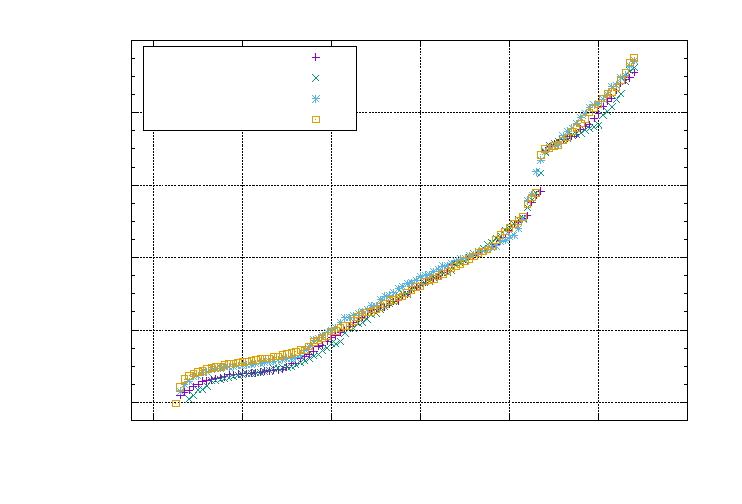
\includegraphics{kovegenv}}%
    \gplfronttext
  \end{picture}%
\endgroup

    \caption{Egenvärden till kovariansmatrisen från \eqref{eq:C} för fyra olika strängar. Det största egenvärdent ses vara åtminstone $10^{16}$ storlekar större än det minsta, vilket påvisar en signifikant skillnad i bidrag till rörelsen från vardera egenmod.}
    \label{fig:kovegenvarde}
\end{figure}

\begin{figure}
    \centering
    % GNUPLOT: LaTeX picture with Postscript
\begingroup
  \makeatletter
  \providecommand\color[2][]{%
    \GenericError{(gnuplot) \space\space\space\@spaces}{%
      Package color not loaded in conjunction with
      terminal option `colourtext'%
    }{See the gnuplot documentation for explanation.%
    }{Either use 'blacktext' in gnuplot or load the package
      color.sty in LaTeX.}%
    \renewcommand\color[2][]{}%
  }%
  \providecommand\includegraphics[2][]{%
    \GenericError{(gnuplot) \space\space\space\@spaces}{%
      Package graphicx or graphics not loaded%
    }{See the gnuplot documentation for explanation.%
    }{The gnuplot epslatex terminal needs graphicx.sty or graphics.sty.}%
    \renewcommand\includegraphics[2][]{}%
  }%
  \providecommand\rotatebox[2]{#2}%
  \@ifundefined{ifGPcolor}{%
    \newif\ifGPcolor
    \GPcolortrue
  }{}%
  \@ifundefined{ifGPblacktext}{%
    \newif\ifGPblacktext
    \GPblacktexttrue
  }{}%
  % define a \g@addto@macro without @ in the name:
  \let\gplgaddtomacro\g@addto@macro
  % define empty templates for all commands taking text:
  \gdef\gplbacktext{}%
  \gdef\gplfronttext{}%
  \makeatother
  \ifGPblacktext
    % no textcolor at all
    \def\colorrgb#1{}%
    \def\colorgray#1{}%
  \else
    % gray or color?
    \ifGPcolor
      \def\colorrgb#1{\color[rgb]{#1}}%
      \def\colorgray#1{\color[gray]{#1}}%
      \expandafter\def\csname LTw\endcsname{\color{white}}%
      \expandafter\def\csname LTb\endcsname{\color{black}}%
      \expandafter\def\csname LTa\endcsname{\color{black}}%
      \expandafter\def\csname LT0\endcsname{\color[rgb]{1,0,0}}%
      \expandafter\def\csname LT1\endcsname{\color[rgb]{0,1,0}}%
      \expandafter\def\csname LT2\endcsname{\color[rgb]{0,0,1}}%
      \expandafter\def\csname LT3\endcsname{\color[rgb]{1,0,1}}%
      \expandafter\def\csname LT4\endcsname{\color[rgb]{0,1,1}}%
      \expandafter\def\csname LT5\endcsname{\color[rgb]{1,1,0}}%
      \expandafter\def\csname LT6\endcsname{\color[rgb]{0,0,0}}%
      \expandafter\def\csname LT7\endcsname{\color[rgb]{1,0.3,0}}%
      \expandafter\def\csname LT8\endcsname{\color[rgb]{0.5,0.5,0.5}}%
    \else
      % gray
      \def\colorrgb#1{\color{black}}%
      \def\colorgray#1{\color[gray]{#1}}%
      \expandafter\def\csname LTw\endcsname{\color{white}}%
      \expandafter\def\csname LTb\endcsname{\color{black}}%
      \expandafter\def\csname LTa\endcsname{\color{black}}%
      \expandafter\def\csname LT0\endcsname{\color{black}}%
      \expandafter\def\csname LT1\endcsname{\color{black}}%
      \expandafter\def\csname LT2\endcsname{\color{black}}%
      \expandafter\def\csname LT3\endcsname{\color{black}}%
      \expandafter\def\csname LT4\endcsname{\color{black}}%
      \expandafter\def\csname LT5\endcsname{\color{black}}%
      \expandafter\def\csname LT6\endcsname{\color{black}}%
      \expandafter\def\csname LT7\endcsname{\color{black}}%
      \expandafter\def\csname LT8\endcsname{\color{black}}%
    \fi
  \fi
    \setlength{\unitlength}{0.0500bp}%
    \ifx\gptboxheight\undefined%
      \newlength{\gptboxheight}%
      \newlength{\gptboxwidth}%
      \newsavebox{\gptboxtext}%
    \fi%
    \setlength{\fboxrule}{0.5pt}%
    \setlength{\fboxsep}{1pt}%
\begin{picture}(6802.00,3968.00)%
    \gplgaddtomacro\gplbacktext{%
      \csname LTb\endcsname%
      \put(980,640){\makebox(0,0)[r]{\strut{}$10^{-13}$}}%
      \csname LTb\endcsname%
      \put(980,1669){\makebox(0,0)[r]{\strut{}$10^{-12}$}}%
      \csname LTb\endcsname%
      \put(980,2698){\makebox(0,0)[r]{\strut{}$10^{-11}$}}%
      \csname LTb\endcsname%
      \put(980,3727){\makebox(0,0)[r]{\strut{}$10^{-10}$}}%
      \csname LTb\endcsname%
      \put(1100,440){\makebox(0,0){\strut{}$0$}}%
      \csname LTb\endcsname%
      \put(2435,440){\makebox(0,0){\strut{}$0,5$}}%
      \csname LTb\endcsname%
      \put(3771,440){\makebox(0,0){\strut{}$1$}}%
      \csname LTb\endcsname%
      \put(5106,440){\makebox(0,0){\strut{}$1,5$}}%
      \csname LTb\endcsname%
      \put(6441,440){\makebox(0,0){\strut{}$2$}}%
    }%
    \gplgaddtomacro\gplfronttext{%
      \csname LTb\endcsname%
      \put(160,2183){\rotatebox{-270}{\makebox(0,0){\strut{}$\ev{b_{i}(t)b_{i}(t+\Delta t)}$}}}%
      \put(3770,140){\makebox(0,0){\strut{}$\Delta t$ /[s]}}%
      \csname LTb\endcsname%
      \put(2580,1055){\makebox(0,0)[r]{\strut{}$\tau_1=\unit[7,24]{s}$}}%
      \csname LTb\endcsname%
      \put(2580,835){\makebox(0,0)[r]{\strut{}$\tau_2=\unit[2,52]{s}$}}%
      \csname LTb\endcsname%
      \put(4179,1055){\makebox(0,0)[r]{\strut{}$\tau_3=\unit[1,16]{s}$}}%
      \csname LTb\endcsname%
      \put(4179,835){\makebox(0,0)[r]{\strut{}$\tau_4=\unit[0,61]{s}$}}%
      \csname LTb\endcsname%
      \put(5778,1055){\makebox(0,0)[r]{\strut{}$\tau_5=\unit[0,31]{s}$}}%
      \csname LTb\endcsname%
      \put(5778,835){\makebox(0,0)[r]{\strut{}$\tau_6=\unit[0,32]{s}$}}%
    }%
    \gplbacktext
    \put(0,0){\includegraphics{korrfil3}}%
    \gplfronttext
  \end{picture}%
\endgroup

    \caption{}
    \label{fig:korrelation}
\end{figure}

\begin{figure}
    \centering
    \input{bilder/strangar/moder.tex}
    \caption{}
    \label{fig:egenmoder}
\end{figure}

\begin{figure}
    \centering
    \input{bilder/strangar/modkorrektion.tex}
    \caption{}
    \label{fig:modkorrektion}
\end{figure}


\begin{figure}\centerline{
\subfigure[][]{
\input{bilder/strangar/ktauconf.tex}
}
\subfigure[][]{
\input{bilder/strangar/ktaunonconf.tex}
}}
\caption{}
\label{fig:ktau}
\end{figure}

%Resultat som kan tas med

%Motivera att jämviktsläge fanns
%Uppdelningen i egenmoder, olika relaxationstid
%Dispersionsrelation?
%Skillnad mellan confined och unconfined



\section{Diskussion}

Nedan finns förslag på rubriker, ändra gärna och lägg till

\subsection{Polynomanpassningens påverkan på resultatet}

\subsection{Strängen verkar vibrera kring ett jämviktläge}

\subsection{Skillnad mellan non-confined och confined}

\subsection{hur $L_{p}>>L_{sträng}$ påverkar resultaten}


%Bara en liten kodsnutt som behövs när man kompilerar lokalt
%%% Local Variables: 
%%% mode: latex
%%% TeX-master: "00main.tex"
%%% End: 

%\chapter{Slutsats}



%Bara en liten kodsnutt som behövs när man kompilerar lokalt
%%% Local Variables: 
%%% mode: latex
%%% TeX-master: "00main.tex"
%%% End: 

%%%%%%%%%%%%%%%%%%%%%%%%% Källförteckning %%%%%%%%%%%%%%%%%%%%%%%%%
\newpage
\bibliographystyle{ieeetr}
\bibliography{referenser_kandidat}

%%%%%%%%%%%%%%%%%%%%%%%%%%%%% Bilagor %%%%%%%%%%%%%%%%%%%%%%%%%%%%%
\clearpage

\appendix


%\chapter{Förklaringsordlista}

%I den här bilagan finns en lista över de lite

\begin{description}[align=left]

\item[Asfärisitet] Ett mått på sfärisk symmetri betecknat $A$. Fullständig sfärisk symmetri fås för $A=0$ medan en uttalat utdragen form fås mot gränsen $A=1$.

\item[Confined] Sträng placerad i mikrokanal.

\item[CTRW] Continuous time random walk, sv. tidskontinuerlig slumpvandring, en modell för partikelrörelser.

\item[Cytoplasma] Vätskan innanför cellens yttre  cellmembran/cellvägg var i organeller och andra strukturer och partiklar befinner sig i.

%\item[Energydepleted] Celler i dvala.

\item[fBm] fractional Brownian motion, sv. , modell för att beskriva stokastiska processer med inbyggd bestående korrelation mellan stegen.

\item[Filament] Kedja av ihopkopplade proteiner.

\item[fGn] fractional Gaussian noise, stegen i fBm.

\item[Log-fas] Aktiva celler i en koloni som är i ett stadie av celldelning.

\item[MSD] Mean squared displacement, sv. medelvärde av kvadrerad förflyttning.

\item[Non-confined] Fri sträng.

\item[Persistence length] Karakteristisk längd för strängarna som relaterar till tangentkorrelationen.

\item[PSD] Power spectral density, sv. spektrala effekttätheten.

%\item[Random Walk] sv. slumpvandring, en diskret rörelse med statistiskt oberoende, normalfördelade steg.

\item[SDE] Stokastisk differentialekvation.

\item[WLC] Worm-like chain, sv. masklik kedja, en modell för att beskriva polymerers dynamik.

%Ska vi ha även ha: stokastisk, passiv transport?

\end{description}



%Bara en liten kodsnutt som behövs när man kompilerar lokalt
%%% Local Variables: 
%%% mode: latex
%%% TeX-master: "00main.tex"
%%% End: 

%\chapter{Kompletterande beräkningar kring skattning av väntevärde och varians}
\label{sec:noggrannhet}

I den här bilagan bevisas att skattningarna i avsnitt~\ref{sec:diskret_data} är väntevärdesriktiga och hur stor varians man får i respektive skattning.

För att göra beräkningar av hur bra skattningarna är betraktas i båda fallen en uppsättning likafördelade oberoende stokastisk variabler $X_i$ med väntevärde $\mu$ standardavvikelse $\sigma$. Med dessa stokastiska variabler kan man bilda en stokastisk motsvarighet\footnotemark{} till \eqref{eq:mean} och \eqref{eq:standard_error}. Det är sedan dessa stokastiska motsvarigheter som används i beräkningarna nedan. 

\footnotetext{Här används stokastiska variabler som motsvarar skattningarna i avsnitt~\ref{sec:diskret_data}. Detta är för att kunna göra stokastiska beräkningar. Det är värt att betona skattningarna i \eqref{eq:mean} och \eqref{eq:standard_error} är skattningar med hjälp av redan tagna mätvärden $x_i$, som när de har \emph{fått värden} inte längre är stokastiska variabler. }


\section{Skattning av väntevärde}
Medelvärdet i \eqref{eq:mean} blir alltså den nya stokastiska variabeln
\begin{equation}
\bar{X} = \frac{1}{N} \sum_{i=1}^N X_i = \sum_{i=1}^N \frac{X_i}{N}.
\end{equation}
Här ifrån kan väntevärde och varians av $\bar{X}$ enkelt beräknas. Med väntevärdets linjäritet, \eqref{eq:EV_linkomb}, och regeln för vaiansen av en linjärkomination, \eqref{eq:VAR_linkomb}, erhålls
\begin{equation}
\ev{\bar{X}} = \sum_{i=1}^N \frac{\ev{X_i}}{N} = \mu
\end{equation}
och
\begin{equation}
\VAR{\bar{X}} = \sum_{i=1}^N \frac{\VAR{X_i}}{N^2} = \frac{\sigma}{N}.
\end{equation}

Som förväntat förblir väntevärdet av medelvärdet oförändrat, men det anmärkningsvärda här är att variansen i medelvärdet minskar med antalet termer som medelvärderas. Detta betyder att medelvärdets standardavvikelse går som $\sigma/\sqrt{N}$.
Från detta kan man dra slutsatsen att skattningen av väntevärdet i \eqref{eq:mean} bör närma sig det verkliga värdet med en osäkerhet i storleksordningen $\sigma/\sqrt{N}$. 

Hur många termer man bör använda i \eqref{eq:mean} beror på hur noggran skattning man vill få i slutändan. Alternativt begränsas $N$ av hur mycket experimentell data man har tillgång till; i så fall kan man använda \eqref{eq:standard_error} för att uppskatta hur noggrant ens medelvärde blir. 


\section{Skattning av varians}
Här används den stokastiska motsvarigheten till \eqref{eq:standard_error}
\begin{equation}\label{eq:S_square}
S^2 = \frac{1}{N-1} \sum_{i=1}^N \left(X_i-\bar{X} \right)^2.
%=\sum_{i=1}^N \hat{X}^2 
\end{equation}
Nu behöver väntevärde och standardavvikelse beräknas. 

Väntevärdet av $S^2$ fås av att utveckla kvadraterna i \eqref{eq:S_square} och använda väntevärdets linjäritet, \eqref{eq:EV_linkomb}. Då erhålls
\begin{equation}\label{eq:EV_S_square1}
\begin{aligned}
(N-1)\ev{S^2} &=  \sum_{i=1}^N \ev{X_i^2} 
+ \sum_{i=1}^N\ev{\bar{X}^2} 
- 2\sum_{i=1}^N\ev{X_i\,\bar{X}}\\
&= 
\sum_{i=1}^N \Big( \VAR{X_i}+\mu^2 \Big)
+\sum_{i=1}^N\Big( \VAR{\bar{X}}+\mu^2 \Big)
-\frac{2}{N}\sum_{i=1}^N\ev{X_i\,\sum_{j=1}^N X_j}.
\end{aligned}
\end{equation}
Här utnyttjas sen att $X_i$ är en uppsättning \emph{oberoende} stokastiska variabler, varför $\ev{X_i\,X_j}=\COV{X_i}{X_j}+\mu^2=\VAR{X_i}\delta_{ij}+\mu^2$ där $\delta_{ij}$ är ett Kroneckerdelta. Med detta kan \eqref{eq:EV_S_square1} skrivas om till
\begin{equation}\label{eq:EV_S_square2}
\begin{aligned}
\ev{S^2} &= \frac{
N\sigma^2 + N\frac{\sigma^2}{N} + 2N\mu^2
-\frac{2}{N} \left( N\sigma^2 + N^2\mu^2 \right)
}{N-1} \\
&= \sigma^2.
\end{aligned}
\end{equation}
Härmed är det bevisat att \eqref{eq:standard_error} är obiaserad i väntevärdesmening -- alltså att Bessels korrektion stämmer.


Med väntevärdet beräknat kan nu variansen av $S^2$ fås med hjälp av 
\begin{equation}\label{eq:VAR_S_square}
\VAR{S^2} = \ev{\left(S^2\right)^2} - \ev{S^2}^2
= \frac{1}{(N-1)^2}\ev{\left(\sum_{i=1}^N\left(X_i-\bar{X}\right)^2 \right)^2} - \sigma^4.
\end{equation}
Det som behöver redas ut här är summatermen ovan. 
Det går tyvärr inte att beräkna den exakt utan att veta $X_i$:s fördelning, men för stora $N$ kan man uppskatta den. 

Till att börja med kan kvadraten av summan skrivas om till
\begin{equation}
\ev{\left(\sum_{i=1}^N\left(X_i-\bar{X}\right)^2 \right)^2} 
= \sum_{i=1}^N \sum_{j=1}^N
\ev{ \left(X_i-\bar{X}\right)^2\left(X_j-\bar{X}\right)^2 }.
\end{equation}
Hade de två faktorerna här varit statistiskt oberoende blir väntevärdet av produkten samma som produkten av väntevärdena\cite{Rice_matstat2006}. Så är tyvärr inte fallet eftersom $\bar{X}$ beror av alla $X_i$.

För att kunna jobba vidare används approximationen att sätta $\bar{X}\approx \mu$, vilket ju sen tidigare visade sig fungera bra för stora $N$. Detta ger att de två faktorerna blir oberoende för $i\neq j$ eftersom $X_i$ var satta att vara en uppsättning oberoende stokastiska variabler. Nu kan summan skrivas om till
\begin{equation}\label{eq:sum_of_moments}
\ev{\left(\sum_{i=1}^N\left(X_i-\bar{X}\right)^2 \right)^2} 
\approx
\sum_{i=1}^N \ev{\left(X_i-\mu \right)^4} 
+\sum_{i=1}^N\sum_{j\neq i} 
\ev{\left(X_i-\mu \right)^2}\ev{\left(X_j-\mu \right)^2}.
\end{equation}
Dubbelsumman är inga problem att evaluera; den innehåller bara varianserna multiplicerade. Däremot behövs mer information om hur $X_i$ är fördelade för att kunna säga något om den första summan -- som är över fjärdemomenten.

Här behöver nästa approximation införas. Den bygger också på att $N$ är stort. Eftersom dubbelsumman innehåller i storleksordningen $N^2$ termer medan summan över fjärdemomenten endast är över $N$ termer, så kommer dubbelsumman att dominera för stora $N$. Detta gör att \eqref{eq:sum_of_moments} kan approximeras med
\begin{equation}\label{eq:EV_squared_sum}
\ev{\left(\sum_{i=1}^N\left(X_i-\bar{X}\right)^2 \right)^2} 
\approx
N^2\sigma^4.
\end{equation}
Man kan motivera att sätta $N^2$, istället för $(N^2-N)$, med att säga att fjärdemomenten alltid är positiva så att man får en underskattning av att helt bortse från den summan. Samtidigt så är det rimligt att anta att $\ev{\left(X_i-\mu\right)^4}\approx\sigma^4$, alltså att de är i samma storleksordning som variansen i kvadrat. Tillsammans ger detta $N^2\sigma^4$.

Slutligen erhålls nu en uppskattning av variansen av $S^2$. Så om man kombinerar \eqref{eq:VAR_S_square} med \eqref{eq:EV_squared_sum} fås för stora $N$: 
\begin{equation}
\VAR{S^2} 
\approx \sigma^4\left(\frac{N^2}{(N-1)^2} -1 \right) 
=\sigma^4\frac{2N-1}{(N-1)^2}
\approx \frac{2}{N}\sigma^4.
\end{equation}
Även här syns att \emph{variansen} av skattningen av variansen minskar som $1/N$, vilket betyder att \emph{standardavvikelsen} av skattningen av variansen går som $1/\sqrt{N}$. 


%Bara en liten kodsnutt som behövs när man kompilerar lokalt
%%% Local Variables: 
%%% mode: latex
%%% TeX-master: "00main.tex"
%%% End: 

%\chapter{CTRW och subdiffusion}
\todo{Sidnumrering i appendix stämmer inte?}

Continous time random walk är modell där rörelsen beskrivs av 
\begin{equation}
    X(t) = \sum_{i=1}^{n(t)} x_i
\end{equation}
där $x_i$ identiskt oberoende fördelade steg med sannolikhetsfördelning $p(x)$. Till skillnad mot en enklare slumpvandring så sker inte stegen med jämna tidsintervall, utan tiden mellan stegen är slumpmässiga med en sannolikhetsfördelning $\psi (t)$. Vidare betecknas sannolikheten att $n$ stycken steg har skett efter en tid $t$ som $P'(n,t)$ och $p_n(x)$ som sannolikheten att befinna sig vid $x$ efter $n$ stycken steg. Givet dessa definitioner är sannolikheten att befinna sig vid $x$ efter en tid $t$ precis 
\begin{equation}
\label{eq:P(x,t)}
    P(x,t) =\sum_{n=0}^{\infty} P'(n,t)p_n(x).
\end{equation}

För att beräkna godtyckliga moment av $X(t)$, av speciellt intresse är väntevärdet och variansen, så betraktar vi fouriertransformen av $P(x,t)$
\begin{equation}\label{eq:four}
\tilde{P}(k,t) = \int_{-\infty}^{\infty} P(x,t)\ee^{\ii kx}dx.
\end{equation}
Från fouriertransformen kan godtyckligt moment beräknas enligt 
\begin{equation}\label{eq:moment}
\ev{X(t)^n} = (-i)^n\frac{\pd^n \tilde{P}(k,t)}{\pd k^n}\big |_{k=0}
\end{equation}. 

Det visar sig att 
\begin{equation}
p_n(x) = p(x)*p(x)...*p(x),
\end{equation}
där $*$ betecknar faltning och $p(x)$ är faltad $n$ gånger med sig själv. \todo{motivera} Således är 
\begin{equation}\label{eq:Pfour}
P(k,t) =\sum_{n=0}^{\infty} P'(n,t)p(k)^n,
\end{equation}
där $p(k)$ är fouriertransformen av $p(x)$ och vi har utnyttjat faltning av två funktioner i $x$-rummet motsvarar multiplikation i $k$-rummet. Det underlättar nu genom att beskriva $P'(n,t)$ i termer av sannolikhetsfördelningen $\psi (t)$ som enligt motsvarar sannolikheten att ett steg sker efter en tid $t$. Detta görs enklast genom att notera att sannolikheten att inget steg sker under en tid $t$ är 
\begin{equation}\label{eq:nojump}
\Psi (t) = 1-\int_0^t \psi(t')dt' = \int_t^{\infty} \psi(t)dt. 
\end{equation}
Givet detta är sannolikheten att ett steg sker under en tid $t$
\begin{equation}
P'(1,t) = \int_0^t\psi(t')\Psi(t-t')dt',
\end{equation}
där vi alltså summerar sannolikheten att ett steg sker vid $t'$ och sedan inget mer under en tid $t-t'$ över alla $t'$. Således är $P'(1,t) = \psi(t)*\Psi(t)$ och från detta inses
\begin{equation}
P(n,t) = \psi(t)*\psi(t)*...*\psi(t)*\Psi(t).
\end{equation}
Detta uttryck kan förenklas genom ensidig laplacetransformera i $t$ enligt 
\begin{equation}
P'(n,s) = \int_0^\infty P'(n,t)\ee^{-st},
\end{equation}
vilket ger 
\begin{equation}
P(n,s) = \psi(s)^n\Psi(s),
\end{equation}
där $\psi(s)$ är laplacetransformen av $\psi(t)$ och likvärdigt för $\Psi(s)$ samt. Från definitionen \eqref{eq:nojump} fås 
\begin{equation}
\Psi(s) = \frac{1-\psi(s)}{s}.
\end{equation}
Vi är nu redo att presentera \eqref{eq:four} där vi utnyttjar laplacetransformen av $P(n,t)$ vilket ger 
\begin{equation}
P(k,s) = \sum_{n=0}^{\infty} \frac{1-\psi(s)}{s}[\psi(s)p(k)]^n,
\end{equation}
och slutligen med hjälp av en geometrisk summa får vi 
\begin{equation}\label{eq:master}
P(k,s) = \frac{1-\psi(s)}{s}\frac{1}{1-\psi(s)p(k)}.
\end{equation}

Genom att applicera \eqref{eq:moment} på detta samband kan väntevärdet samt variansen för $X(t)$ beräknas vilket visas nedan. Väntevärdet blir 
\begin{equation}
\ev{X(s)} = -i\frac{\pd \tilde{P}(k,s)}{\pd k}\big |_{k=0},
\end{equation}
som med \eqref{eq:master} ger 
\begin{equation}
\ev{X(s)} = \frac{1-\psi(s)}{s}\frac{\psi(s)(-i\frac{\pd p(k)}{\pd k})}{(1-\psi(s)p(k))^2}\bigg |_{k=0}.
\end{equation}
och ser vid en första anblick inte ut som framsteg. Men uttrycket förenklas genom att inse att 
\begin{equation}
(-i\frac{\pd p(k)}{\pd k})\bigg |_{k=0} = \ev{x}, \quad p(k)\bigg |_{k=0} = 1. 
\end{equation}
Väntevärdet blir således 
\begin{equation}\label{eq:medel}
\ev{X(s)} = \frac{\psi(s)\ev{x}}{s(1-\psi(s))},
\end{equation}
med antagandet $\ev{x}\equiv l< \infty$. Analogt kan variansen beräknas enligt 
\begin{equation}
\ev{X(s)^2} = -\frac{\pd^2 \tilde{P}(k,s)}{\pd k^2}\bigg |_{k=0},
\end{equation}
vilket efter en liten exercis ger 
\begin{equation}\label{eq:var}
\ev{X(s)^2} = \frac{\ev{x^2}\psi(s)}{s(1-\psi(s))}+\frac{2\ev{x}\psi(s)}{s(1-\psi(s))^2},
\end{equation}
där $\ev{x^2}\equiv \sigma_x^2< \infty$. Vi har således uttryck väntevärdet samt variansen för $X(s)$ i termer av transformen av sannolikhetsfördelningen $\psi(t)$. 

\todo[inline]{exempel på normal samt anomal diffusion kommer nedan.}
\section{Normal diffusion}
Vid normal diffusion är väntetiden $\tau\equiv\ev{t}$ finit och väntevärde samt varians kan beräknas i gränsen då $t\to\infty$ vilket är ekvivalent med $s\to0$. I denna gräns gäller sannolikhetsfördelning 
\begin{equation}
\psi(s) \sim 1-\tau+s+\frac{\ev{t^2}s^2}{2} 
\end{equation}



%\chapter{Fördjupning i fBm och fGn}
\label{sec:App_fBm}

\todo[inline]{Inga tomma rubriker}

\section{Definition}

Varje fractional Brownian motion (fBm) är kopplad till en parameter $H$ kallad Hurstparametern, $0<H<1$, som är med och avgör många av rörelsens egenskaper. Ett sätt att formellt representera fBm är att utgå från en vanlig brownsk rörelse $B(t)$, som matematiskt beskrivs av en Wienerprocess, och vikta tidigare steg i rörelsen med $(t-t')^{H-\nicefrac{1}{2}}$, dör $t$ och $t'$ är olika tidpunkter, så att fBm:n blir ett glidande medelvärde av $\dd{B}(t)$ enligt \cite{Mandelbrot_fBm1968}
\begin{equation} \label{eq:fBm_repr}
\begin{aligned}
    B_H(t,\Omega)=& \frac{1}{\Gamma(H+\nicefrac{1}{2})}
    \int_{\infty}^0 \left( \abs{t-t'}^{H-\nicefrac{1}{2}}-\abs{-t}^{H-\nicefrac{1}{2}}\right)\,\dd{B}(t',\Omega) \\
    &+ \int_0^t \abs{t-t'}^{H-\nicefrac{1}{2}} \dd{B}(t',\Omega)
\end{aligned}
\end{equation}
utgående från startposition i 0 där $\Omega$ representerar mängden av alla möjliga värden för den stokastiska funktionen och $\Gamma$ är gammafunktionen. För en beskrivning av hur denna typ av integral med stokastisk integrationsvariabel kan beräknas, hänvisas till någon grundläggande lärobok i stokastisk analys, exempelvis \cite{Oksendal2002}.

%Denna representation är dock inte unik \cite{Dieker_fBm}.

En normaliserad fBm, $B_H(t)$, karakteriseras fullständigt av följande fem egenskaper~\cite{Dieker_fBm}
\begin{subequations}
\begin{align} 
    B_H(0)&=0 \\ 
    B_H(t+1)-B_H(t) &\sim N(0,1)\qcomma \forall t \label{eq:fBm_normstep}\\
    \ev{B_H(t)}&=0 \label{eq:fBm_mean} \\
    \ev{B^2_H(t)}&=\abs{t}^{2H} \label{eq:fBm_var}\\
    \ev{(B_H(t_1)-B_H(t_2))^2}&=\abs{t_1-t_2}^{2H}  \label{eq:fBm_stat_step}
\end{align}
\end{subequations}
där $t>0$ och $H$ är den tidigare presenterade Hurstparametern. \todo[color=lime]{Visa varför detta måste gälla} Relationen i \eqref{eq:fBm_stat_step} medför att rörelsen har stationära steg. Stegen, som funktion av tid, mellan positionerna $B_H(t)$ och $B_H(t+T)$
\begin{equation} \label{eq:fracGauss}
    \delta(t) = B_H(t+T) - B_H(t)
\end{equation}
kallas \emph{fractional Gaussian noise} (fGn). Här är $T$ tiden mellan två samplingar i en mätserie. 

Om fBm:n inte normeras utan definieras direkt från \eqref{eq:fBm_repr} kan man visa att variansen för \emph{icke-normerade} fBm:n $\hat{B}_H(t)$, motsvarande egenskap \eqref{eq:fBm_var}, blir \cite{Dieker_fBm}
\begin{equation} \label{eq:fBm_onorm_var}
    \ev{\hat{B}^2_H(t)} = V_H \abs{t}^{2H},
\end{equation}
där $V_H = \Gamma(1-2H)\frac{\cos(\pi H)}{\pi H}$ \cite{Flandrin_fBmspektrum1989}.


\section{Korrelationer}
\todo[color=lime]{Ändra $\gamma$ och $\Delta$}
Kovariansen för fBm fås genom att utnyttja egenskaper för kovarians \eqref{eq:COV} enligt
\begin{equation}
\begin{aligned}
    \COV{B_H(t)}{B_H(t+\Delta{t})}&=\ev{B_H(t)B_H(t+\Delta{t})}-\ev{B_H(t)}\ev{B_H(t+\Delta{t})}
    \\
    &=\ev{B_H(t)B_H(t+\Delta{t})},
\end{aligned}
\end{equation}
där $\ev{B_H(t)}=\ev{B_H(t+\Delta{t})}=0$ enligt \eqref{eq:fBm_mean}. För att beräkna det resterande väntevärdet av produkten kan man utnyttja sambandet $(B_H(t)-B_H(t+\Delta{t}))^2=B_H(t)^2 -2B_H(t)B_H(t+\Delta{t})+B_H(t+\Delta{t})^2$ för att få
\begin{equation}
    \ev{B_H(t)B_H(t+\Delta{t})}
    =\frac{
    \ev{B_H(t)^2} + \ev{B_H(t+\Delta{t})^2} - \ev{(B_H(t)-B_H(t+\Delta{t}))^2}
    }{2}.
\end{equation}
Med \eqref{eq:fBm_var} och \eqref{eq:fBm_stat_step} fås tillslut kovariansen
\begin{equation} \label{eq:fBm_cov}
    \COV{B_H(t)}{B_H(t+\Delta{t})} = \frac{1}{2}\left(\abs{t}^{2H}+\abs{t+\Delta t}^{2H}-\abs{\Delta{t}}^{2H}\right).
\end{equation}
Kovariansen för en fBm är alltså tidsberoende och processen är därmed icke-stationär. 

Detta resultat kan dock användas för att beräkna kovariansen mellan stegen, fGn, definierade i \eqref{eq:fracGauss}. På samma sätt som för kovariansen av fBm har stegen medelvärde 0 enligt  \eqref{eq:fBm_normstep} vilket ger
\begin{equation}
    \COV{\delta(t_1)}{\delta(t_2)} = \Big\langle(B_H(t_1+T)-B_H(t_1))(B_H(t_2+T)-B_H(t_2))\Big\rangle.
\end{equation}
Här är $T$ tiden mellan två samplingspunkter. Om produkten utvecklas till fyra termer kan kovariansen i \eqref{eq:fBm_cov} användas för att få fram följande kovarians för fGn:
\begin{equation} \label{eq:fGn_cov}
    \COV{\delta(t)}{\delta(t+\Delta{t})} 
    = \frac{1}{2}
    \left(-2\abs{\Delta{t}}^{2H}+\abs{\Delta{t}+T}^{2H}+\abs{\Delta{t}-T}^{2H}\right) 
    \equiv \kappa(\Delta{t}),
\end{equation}
där $\Delta{t}=\abs{t_1+t_2}$.
Detta beror enbart av tidsseparationen mellan $t_1$ och $t_2$, vilket förväntas från en stationär fördelning.


\section{PSD för icke-stationära processer}
\todo[color=lime]{Ändra från WVS till S?}
Som man kan se i avsnitt~\ref{sec:PSD} beror PSD:n enbart på frekvensen och kan beräknas för stationära processer. Konceptet med PSD kan dock generaliseras till icke-stationära processer via Wigner-Ville-spektrumet (WVS) för en process $x(t)$ med kovariansfunktion $\gamma_x(t_1,t_2)$ \cite{Flandrin_fBmspektrum1989}. Wigner-Ville-spektrumet definieras som
\begin{equation} \label{eq:WVS}
V_x(t,\omega)=
\int^{\infty}_{-\infty} 
\kappa_x\left(t{+}\nicefrac{\tau}{2},\; t{-}\nicefrac{\tau}{2}\right) \ee^{-\ii \omega \tau} \dd\tau.
\end{equation}
Alltså kan WVS:en vara tidsberoende. 

Det går att visa att WVS övergår i PSD för stationära processer. Detta möjliggör att PSD kan tas fram även för den icke-stationära fBm.


\section{PSD för fGn}
\label{sec:PSD_fGn}

PSD för fGn kan räknas ut med hjälp av dess kovariansfunktion $\kappa(t_1,t_2)=\kappa(\Delta{t})$ i ekvation \eqref{eq:fGn_cov} med $\Delta{t}=t_1-t_2$ och via Wigner-Ville-spektrummet i \eqref{eq:WVS}\todo[color=cyan]{Stökig mening}
\begin{equation}
    V_{\delta}(t,\omega)
    =\int^{\infty}_{-\infty} 
    \kappa_{\delta}
    \left( t+\frac{\tau}{2},t-\frac{\tau}{2} \right) 
    \ee^{-\ii \omega\tau} \dd\tau
\end{equation}
\todo[color=cyan]{?}fås med $\Delta{t}=t+\frac{\tau}{2}-(t-\frac{\tau}{2})=\tau$ vidare
\begin{equation} \label{eq:fGn_covterm}
    V_{\delta}(t, \omega)
    =
    \int^{\infty}_{-\infty} 
    \gamma_{\delta}(\tau) \ee^{-\ii \omega\tau} \dd\tau 
    = 
    \int^{\infty}_{-\infty} \frac{1}{2} 
    \left(
    -2\abs{\tau}^{2H} + \abs{\tau-T}^{2H} + \abs{\tau+T}^{2H}
    \right) 
    \ee^{-\ii \omega\tau} \dd\tau.
\end{equation}
Här kan noteras att WVS:n nu gått över till PSD för en stationärprocess så att $V_{\delta(\omega)}=S(\omega)$ från Wiener-Khinthchine-teoremet i \eqref{eq:W-K-theorem}. Via linjäritetsegenskaper kan integralens tre delar beräknas var för sig. Den första termen utgör fouriertransformen för $\abs{\tau}^{(2H+1)-1}$, $2H\in (0,1)$, vilken återfinns i \cite{BETA}
\begin{equation}
\begin{aligned}
    \int^{\infty}_{-\infty} -\abs{\tau}^{(2H+1)-1}\ee^{-\ii \omega\tau} \dd\tau 
    &= -\frac{
    2\Gamma(2H+1)
    \cos(\frac{(2H+1)\pi}{2})}{
    \abs{\omega}^{2H+1}} 
    \\ 
    &= -2\Gamma{(2H+1)} \cos\left(H\pi+\frac{\pi}{2}\right) \abs{\omega}^{-(2H+1)} 
    \\
    &= 2\Gamma{(2H+1)}\sin(H\pi) \abs{\omega}^{-(2H+1)} \equiv F.
\end{aligned}
\end{equation}
Andra termen kan uttryckas i termer av $F$ med hjälp av variabelbytet $t'=\tau+T$
\begin{equation}
\int^{\infty}_{-\infty}\frac{1}{2} \abs{\tau+T}^{2H})\ee^{-\ii \omega\tau} \dd\tau 
= \frac{1}{2}\int^{\infty}_{-\infty} \abs{t'}^{2H} \ee^{-\ii \omega(t'-T)} \dd\tau 
= -\frac{1}{2} F \ee^{\ii \omega T}.
\end{equation}\todo[color=cyan]{Vart tar $t'$ vägen efter integralen? Det bakas in i F}
Analogt för tredje termen fås $-\frac{1}{2}F\ee^{-\ii \omega T}$. 

Läggs dessa tre termer ihop fås
\begin{equation}
\begin{aligned}
    V_{\delta}(t,\omega)
    &= F\left(1-\frac{1}{2}\left(\ee^{\ii \omega T}+\ee^{-\ii \omega T}\right)\right)
    = F\Big( 1-\cos(\omega T) \Big) 
    = 2F\left(\sin(\frac{\omega T}{2})\right)^2 \\
    &= 
    4\Gamma{(2H+1)}
    \sin(H\pi)\left(\sin(\frac{\omega T}{2})\right)^2 \abs{\omega}^{-(2H+1)}. \label{eq:fGn_PSD_halvklar}
\end{aligned}
\end{equation}
Genom att utnyttja följande egenskaper för gammafunktionen
\begin{align}
\Gamma(1-z)\Gamma(z)&=\frac{\pi}{\sin(\pi z)} \\
\Gamma(z+1)&=z\Gamma(z),
\end{align}
kan gammafaktorn i \eqref{eq:fGn_PSD_halvklar} skrivas om till
\begin{equation}
\Gamma(2H+1) 
= 2 \Gamma(2H) = 2H\frac{\pi}{\sin(2H\pi)}\frac{1}{\Gamma(1-2H)} 
= \frac{H\pi}{\cos(H\pi)\sin(H\pi)\Gamma(1-2H)}.
\end{equation}

För en icke-normerad fBm fås en extra faktor $V_H$, se \eqref{eq:fBm_onorm_var}, i PSD:n för dess fGn: $\hat{\delta}$ enligt
\begin{equation}
V_{\hat{\delta}}(t,\omega) 
= V_H 4\Gamma{(2H+1)}\sin(H\pi) \left( \sin(\frac{\omega T}{2}) \right)^2 \abs{\omega}^{-(2H+1)} 
= 4 \left( \sin(\frac{\omega T}{2}) \right) ^2\abs{\omega}^{-(2H+1)},
\end{equation}
vilken saknar explicit tidsberoende. För $\nicefrac{\omega T}{2} \ll 1$, det vill säga små $\omega$, kan den kvadrerade sinustermen Taylorutvecklas så att
\begin{equation}
    V_{\hat{\delta}}(t,\omega) \approx \frac{ \left( \nicefrac{\omega T}{2} \right)^2 + \mathcal{O}(\omega^4) }{\abs{\omega}^{(2H+1)}}.
\end{equation}
Olika beteende för olika värde på Hurstparametern $H$ framträder nu 
\begin{equation}
    \lim\limits_{\omega \to 0} V_{\hat{\Delta}}(t,\omega) = \begin{cases} 
      0 & H<\nicefrac{1}{2} \\
      \nicefrac{T^2}{4} & H=\nicefrac{1}{2} \\
      \infty & H>\nicefrac{1}{2}
   \end{cases}
\end{equation}
vilket framträder tydligt om PSD:n plottas i dB mot frekvensen.

Tillsist kan nämnas att för en process som förutsäger en kovarians $\propto t^{\alpha}$ ger \eqref{eq:fGn_covterm}-\eqref{eq:fGn_PSD_halvklar} att motsvarande PSD $\propto \omega^{-(\alpha+1)}$.

\todo[color=lime]{Kanske även lägga till för fBm}

\todo[color=lime]{Kanske något om att ej deriverbar}




%Bara en liten kodsnutt som behövs när man kompilerar lokalt
%%% Local Variables: 
%%% mode: latex
%%% TeX-master: "00main.tex"
%%% End: 

%\chapter{Härledning av Langevinekvationen för WLC-modell i mikrokanal}
\label{A5}

I denna bilaga diskuteras övergången från den potentiella energin för WLC-modellen i en mikrokanal 
\begin{equation}\label{eq:Htot}
    \frac{H_\text{tot}}{\kbT}=\int_{0}^{L}\!\dd{s}\,\left[\frac{L_\text{p}}{2}\left(\partial_{s}^{2}\mathbf{r}(s)\right)^2 + \frac{\nu}{2L_\text{p}^3} A(s)^2 + \frac{\mu}{L_\text{p}}\left(\pd_{s}\mathbf{r}(s)\right)^{2} \right]
\end{equation}
till Langevinekvationen 
\begin{equation}\label{eq:wlclangevin}
    \zeta\pd_tA(t,s) = \kbT\left[-L_\text{p}\pd_s^4A(t,s)-\frac{\nu}{L_\text{p}^3}A(t,s)+\frac{2\mu}{L_\text{p}}\pd_s^2A(t,s) \right]+\sigma\pd_tW(t,s).
\end{equation}

Den potentiella energin $H_\text{tot} = H + H_{\text{p}} + H_{\text{f}}$ studeras term för term. I analogi med klassisk mekanik där kraften ges av $-\nicefrac{\dd{V}}{\dd{x}}$ för en potentiell energi $V$, studeras hur den potentiella energi \eqref{eq:Htot} ändras vid en variation $\delta A$, alltså $-\frac{\delta H_\text{tot}}{\delta A}$. Starta med att studera termen $H_{\text{p}} = H_{\text{p}}(A,s)$ där
\begin{equation}
    H_{\text{p}} = \frac{\nu\kbT}{2L_\text{p}^3}\int_0^L\!\dd{s} A(s)^2
\end{equation}
genom att betrakta variationen 
\begin{equation}
    \delta H_{\text{p}} = \frac{\pd H_{\text{p}}}{\pd A}\delta A.
\end{equation}

Detta ger 
\begin{equation}
    \delta H_{\text{p}} = \frac{\nu\kbT}{2L_\text{p}^3}\int_0^L\!\dd{s} 2A(s)\delta A.
\end{equation}
De övriga termerna beror på första- respektive andraderivatan av $A(s)$ vilket kräver lite mer arbete. Starta därför med $H_{\text{f}}=H_{\text{f}}(\pd_sA,s)$ som innehåller förstaderivatan enligt
\begin{equation}
    H_{\text{f}} = \frac{\mu\kbT}{L_\text{p}}\int_0^L\!\dd{s}\left[\pd_s \mathbf{r}(s)\right]^2.
\end{equation}
Eftersom vi inför en variation $\delta A$ i den transversella riktningen kommer inte den tangentiella riktningen förändras, vilket inses efter en kort räkning, vilket motiverar ersättande av $\mathbf{r}(s)$ med $A(s)$ . Denna term ger därför på analogt vis 
\begin{equation}
    \delta H_{\text{f}} = \frac{\pd H_{\text{f}}}{\pd (\pd_s A)}\delta(\pd_sA),
\end{equation}
vilket ger 
\begin{equation}
    \label{eq:deltaHf}
    \delta H_{\text{f}} =  \frac{\mu\kbT}{L_\text{p}}\int_0^L\!\dd{s} 2\pd_sA(s)\delta (\pd_s A).
\end{equation}
Då $H_{\text{f}}$ beror av derivatan $\pd_sA(s)$ ses att $\delta H_{\text{f}}$ innehåller variationen av derivatan av $A(s)$, alltså av termen $\delta (\pd_sA)$. För att komma vidare utnyttjas produktregeln som ger följande relation 
\begin{equation}
    \pd_s\left[\frac{\pd H_{\text{f}}}{\pd \left(\pd_sA\right)}\delta A\right] = \pd_s\left(\frac{\pd H_{\text{f}}}{\pd \left(\pd_sA\right)}\right)\delta A+\frac{\pd H_{\text{f}}}{\pd \left(\pd_sA\right)}\delta(\pd_sA).
\end{equation}
Genom insättning av denna i relation i \eqref{eq:deltaHf} fås 
\begin{equation}
    \delta H_{\text{f}} = \frac{\mu\kbT}{L_\text{p}}\int_0^L\!\dd{s} \left[\pd_s\left[\frac{\pd H_{\text{f}}}{\pd \left(\pd_sA\right)}\delta A\right]-\pd_s\left(\frac{\pd H_{\text{f}}}{\pd \left(\pd_sA\right)}\right)\delta A \right].
\end{equation}
Den första termen i denna ekvation kan nu integreras och genom att kräva att variationen $\delta A$ är noll vid $s=0$ samt $s=L$ försvinner bidraget från denna term. Slutligen fås 
\begin{equation}
    \delta H_{\text{f}} = -\frac{\mu\kbT}{L_\text{p}}\int_0^L\!\dd{s} \pd_s\left(\frac{\pd H_{\text{f}}}{\pd \left(\pd_sA\right)}\right)\delta A,
\end{equation}
och 
\begin{equation}
     \delta H_{\text{f}} = -\frac{\mu\kbT}{L_\text{p}}\int_0^L\!\dd{s} 2\left(\pd_s^2A\right)\delta A.
\end{equation}

För $H$ behöver produktregeln appliceras två gånger, vilket är en följd av att $H = H(\pd_s^2A,s)$ enligt 
\begin{equation}
     H = \frac{ L_\text{p}\kbT}{2}\int_0^L\!\dd{s}\left(\pd_s^2A\right)^2,
\end{equation}
vilket efter en analog beräkning ger 
\begin{equation}
     \delta H = L_\text{p}\kbT \int_0^L\!\dd{s} \pd_s^4A.
\end{equation}

Slutligen studeras variationen av den totala potentiella energin $\delta H_\text{tot} = \delta H + \delta H_{\text{p}} + \delta H_{\text{f}}$ 
\begin{equation}
     \delta H_\text{tot} = \kbT\int_0^L\!\dd{s} \left[L_\text{p}\pd_s^4A+\frac{\nu}{L_\text{p}^3}A -\frac{2\mu}{L_\text{p}}\pd_s^2A\right]\delta A. 
\end{equation}
Kraften på ett längdelement $\dd{s}$ ges då av 
\begin{equation}\label{eq:F}
      F = -\frac{\delta H_\text{tot}}{\delta A} = -\kbT\left[L_\text{p}\pd_s^4A+\frac{\nu}{L_\text{p}^3}A-\frac{2\mu}{L_\text{p}}\pd_s^2A \right]\dd{s} .
\end{equation}
Givet denna kraft kan Newtons andra lag ställas upp enligt 
\begin{equation}
      \rho\dd{s}\pd_t^2A = -\kbT\left[L_\text{p}\pd_s^4A+\frac{\nu}{L_\text{p}^3}A-\frac{2\mu}{L_\text{p}}\pd_s^2A \right]\dd{s},
\end{equation}
där $\rho$ är massan per längdenhet. Detta är en deterministisk rörelseekvation och för att kunna beskriva de stokastiska fluktuationerna på en mikroskopisk sträng används Langevinformalismen. För att få motsvarande Langevinekvation adderas två termer till kraften \cite{Bullerjahn2011,Dhar,VanKampen2007}: en friktionskraft $-\zeta\dd{s}\pd_tA$, där $[\zeta] = \unit[]{[kg/sm]}$ är en friktionskoefficient per längdenhet, samt ett vitt brus $\sigma\pd_t W$, där $\sigma$ är en konstant.

Dividera med $\dd{s}$ enligt 
\begin{equation}
      \rho\pd_t^2A = -\zeta\pd_tA+ \kbT\left[-L_\text{p}\pd_s^4A-\frac{\nu}{L_\text{p}^3}A+\frac{2\mu}{L_\text{p}}\pd_s^2A \right]+\sigma\pd_tW.
\end{equation}
För att slutligen nå ekvation \eqref{eq:wlclangevin} antas att tröghetstermen är försumbar relativt friktionskraften, vilket gäller under antagandet att polymeren är placerad i en vätska med hög viskositet \cite{Dhar} -- alltså att Reynoldstalet är litet. Langevinekvationen för WLC-modellen i en mikrokanal ges därför av
\begin{equation}
    \zeta\pd_tA(t,s) = \kbT\left[-L_\text{p}\pd_s^4A(t,s)-\frac{\nu}{L_\text{p}^3}A(t,s)+\frac{2\mu}{L_\text{p}}\pd_s^2A(t,s) \right]+\sigma\pd_tW(t,s).
\end{equation}



%Bara en liten kodsnutt som behövs när man kompilerar lokalt
%%% Local Variables: 
%%% mode: latex
%%% TeX-master: "00main.tex"
%%% End


\end{document}








%% På svenska ska citattecknet vara samma i både början och slut.
%% Använd två apostrofer (två enkelfjongar): ''.

%% Inkludera PDF-dokument
\includepdf[pages={1-}]{filnamn.pdf} %Filnamnet får INTE innehålla 'mellanslag'!

%% Figurer inkluderade som pdf-filer
\begin{figure}\centering
\centerline{ %centrerar även större bilder
\includegraphics[width=1\textwidth]{filnamn.pdf}
}
\caption{\label{fig:} }
\end{figure}

%% Figurer inkluderade med xfigs "Combined PDF/LaTeX"
\begin{figure}\centering
\resizebox{.8\textwidth}{!}{\input{filnamn.pdf_t}}
\caption{\label{fig:} }
\end{figure}

%% Figurer roterade 90 grader
\begin{sidewaysfigure}\centering
\centerline{ %centrerar även större bilder
\includegraphics[width=1\textwidth]{filnamn.pdf}
}
\caption{\label{fig:} }
\end{sidewaysfigure}


%%Om man vill lägga till något i TOC
\stepcounter{section} %Till exempel en 'section'
\addcontentsline{toc}{section}{\Alph{section}\hspace{8 pt}Labblogg} 



%Bara en liten kodsnutt som behövs när man kompilerar lokalt
%%% Local Variables: 
%%% mode: latex
%%% TeX-master: "00main.tex"
%%% End: 